\documentclass[12pt,a4paper]{report}

\usepackage[top=1in, bottom=1in, left=1.25in, right=1.25in]{geometry}
\usepackage[dvipdfmx]{graphicx}
\usepackage{float}
\usepackage{ctex}
\usepackage{algorithm}
\usepackage{algorithmicx}
\usepackage{algpseudocode}
\usepackage{listings}
\usepackage{color}
\usepackage{tikz}
\usepackage{fancyhdr}
\usepackage{amsmath,amssymb,amsthm}
\usepackage[toc,page]{appendix}
\usepackage{multirow}
\usepackage[utf8]{inputenc}
\usepackage{booktabs}
\usepackage[hidelinks]{hyperref}
\usepackage[center]{caption}
\usepackage[nobiblatex]{xurl}
\usepackage{subfigure}
\usepackage{cite}
\usepackage{xcolor,colortbl}
\usepackage{xparse}
\usepackage{diagbox}
\usepackage{makecell}

\NewDocumentCommand{\code}{v}{%
\texttt{\textcolor{blue}{#1}}%
}

\renewcommand\bibname{References}
\renewcommand\contentsname{Table of Contents}
\renewcommand\figurename{Figure}
\renewcommand\appendixname{Appendix}
\renewcommand\tablename{Table}

\DeclareMathOperator*{\argmax}{arg\,max}

\definecolor{codegreen}{rgb}{0,0.6,0}
\definecolor{codegray}{rgb}{0.5,0.5,0.5}
\definecolor{codepurple}{rgb}{0.58,0,0.82}
\definecolor{backcolour}{rgb}{0.95,0.95,0.92}

\lstset{
	language=Python,
    backgroundcolor=\color{backcolour},   
    commentstyle=\color{codegreen},
    keywordstyle=\color{magenta},
    numberstyle=\tiny\color{codegray},
    stringstyle=\color{codepurple},
    basicstyle=\ttfamily\footnotesize,
    breakatwhitespace=false,         
    breaklines=true,                 
    captionpos=b,                    
    keepspaces=true,                 
    numbers=left,                    
    numbersep=5pt,                  
    showspaces=false,                
    showstringspaces=false,
    showtabs=false,                  
    tabsize=4,
	columns=flexible, 
	emph=[0]{__init__, True, None, Module, Sequential, Conv2d, BatchNorm2d, Tanh, MaxPool2d, FloatTensor, view, ConvTranspose2d, LeakyReLU, Sigmoid, UpsamplingNearest2d, cat, Linear, ModuleList, LSTMCell, exp, randn_like, get_data_loaders, Optional, ToTensor, Compose, BatchNorm1d, DataLoader, tqdm}, 
	emphstyle=[0]\color{blue},
	emph=[1]{nn, np, transforms}, 
	emphstyle=[1]\color{gray},
	emph=[2]{self}, 
	emphstyle=[2]\color{magenta},
	emph=[3]{torch, VggEncoder, VggDecoder, VggLayer, GaussianLstm, __BairRobotPushingDataset, KlAnnealing}, 
	emphstyle=[3]\color{red},
}

\pagestyle{fancy}
\lhead{\leftmark}
\rhead{\labTitle}
\renewcommand{\headrulewidth}{0.5pt}

\def\@maketitle{%
	\newpage
	\null
	\vskip 2em%
	\begin{center}%
	\let \footnote \thanks
    {\LARGE \@title \par}%
    \vskip 1.5em%
    {\large
    	\lineskip .5em%
    	\begin{tabular}[t]{c}% <------
        	\@author%          <------ Authors
      	\end{tabular}\par}%    <------
    \vskip 1em%
    {\large \@date}%
  	\end{center}%
  	\par
  	\vskip 1.5em}

\title{
	
\includegraphics[scale=0.5]{img/nycu_logo.png}\\
	~\\
	\LARGE\textbf{\reportSubtitle}\\
	\Large\textbf{\reportTitle}\\
}
\author{
	\begin{tabular}{rl}
		\textbf{Name: } & \authorName \\
		\textbf{Student ID: } & \authorStudentID  \\
	\end{tabular} \\~\\
	\authorDepartment
}

\newcommand{\reportTitle}{Lab5: Conditional VAE For Video Prediction}
\newcommand{\labTitle}{CVAE For Video Prediction}
\newcommand{\reportSubtitle}{Deep Learning}
\newcommand{\authorName}{許子駿}
\newcommand{\authorStudentID}{311551166}
\newcommand{\authorSchool}{National Yang Ming Chiao Tung University}
\newcommand{\authorDepartment}{Institute of Computer Science and Engineering}

\begin{document}
	\maketitle
	\tableofcontents
	\chapter{Introduction}
\indent
	This task is to solve \textit{LunarLander-v2} and \textit{BreakoutNoFrameskip-v4} using \textbf{deep Q-network (DQN)}, and
	\textit{LunarLanderContinuous-v2} using \textbf{deep deterministic policy gradient (DDPG)}.
	\chapter{Experiment setup}
\indent
    Experiment setup is listed in this chapter including 5 parts, 
    that is, initialization method, activation functions, optimizers, loss function, and the data structure of linear layer.

\section{Initialization method}
\indent
    \textbf{He normal initialization} is used in this experiment (See Listing \ref{he}). \\
    This initialization method performs well empirically when neural networks include \code{ReLU} activation function by many researchers.
    \begin{lstlisting}[language=Python, caption={He normal initialization code.}, label={he}]
    dim_in = layers[i]
    dim_out = layers[i + 1]
    a = np.sqrt(6. / (dim_in + dim_out))
    std = np.sqrt(2. / ((1 + a ** 2) * dim_in))
    
    W = np.random.normal(loc=0., scale=std, size=[dim_out, dim_in])
    b = np.random.normal(loc=0., scale=std, size=[1, dim_out])\end{lstlisting}

\section{Activation functions}
\indent
    There are many activation functions, e.g., \code{LeakyReLU}, \code{ReLU}, \code{Sigmoid}, and etc. 
    In this experiment, 3 activation functions, \code{LeakyReLU}, \code{ReLU} and \code{Sigmoid} 
    (See Figures \ref{leaky-relu}, \ref{relu}, and \ref{sigmoid}), are implemented.

    \begin{figure}[H]
		\centering
		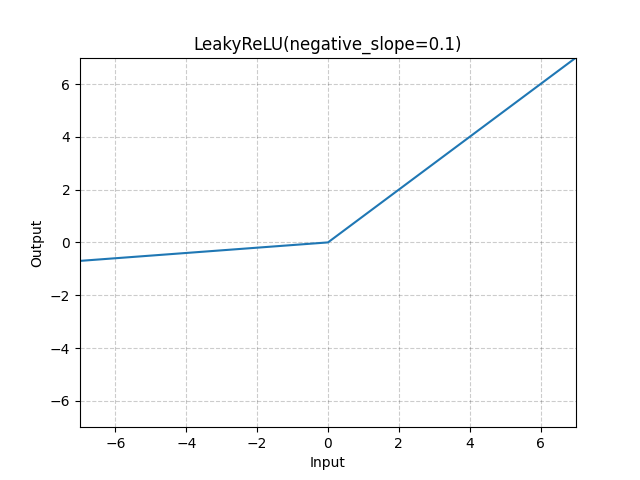
\includegraphics[scale=0.5]{img/leaky-relu.png}
		\caption{Illustration of LeakyReLU activation function.}
		\label{leaky-relu}
	\end{figure}
    \begin{figure}[H]
		\centering
		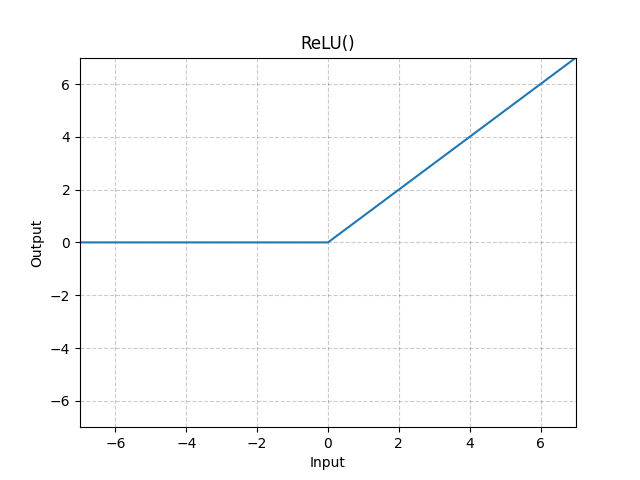
\includegraphics[scale=0.5]{img/relu.png}
		\caption{Illustration of ReLU activation function.}
		\label{relu}
	\end{figure}
    \begin{figure}[H]
		\centering
		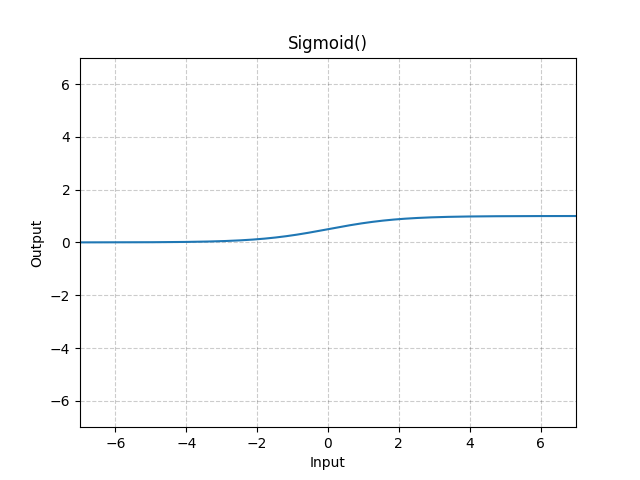
\includegraphics[scale=0.5]{img/sigmoid.png}
		\caption{Illustration of Sigmoid activation function.}
		\label{sigmoid}
	\end{figure}

\section{Optimizers}
\indent
    There are many optimizers, e.g., \code{SGD}, \code{Momentum}, \code{AdaGrad}, \code{Adam}, and etc.
    In this experiment, 2 optimizers, \code{SGD} (vanilla gradient descent in this case) and \code{Adam} (See Figure \ref{adam}) optimizers, are implemented. \\
    \code{Adam} optimizer is mostly used, and it has the great parts of \code{Momentum} and \code{AdaGrad}.

    \begin{figure}[H]
		\centering
		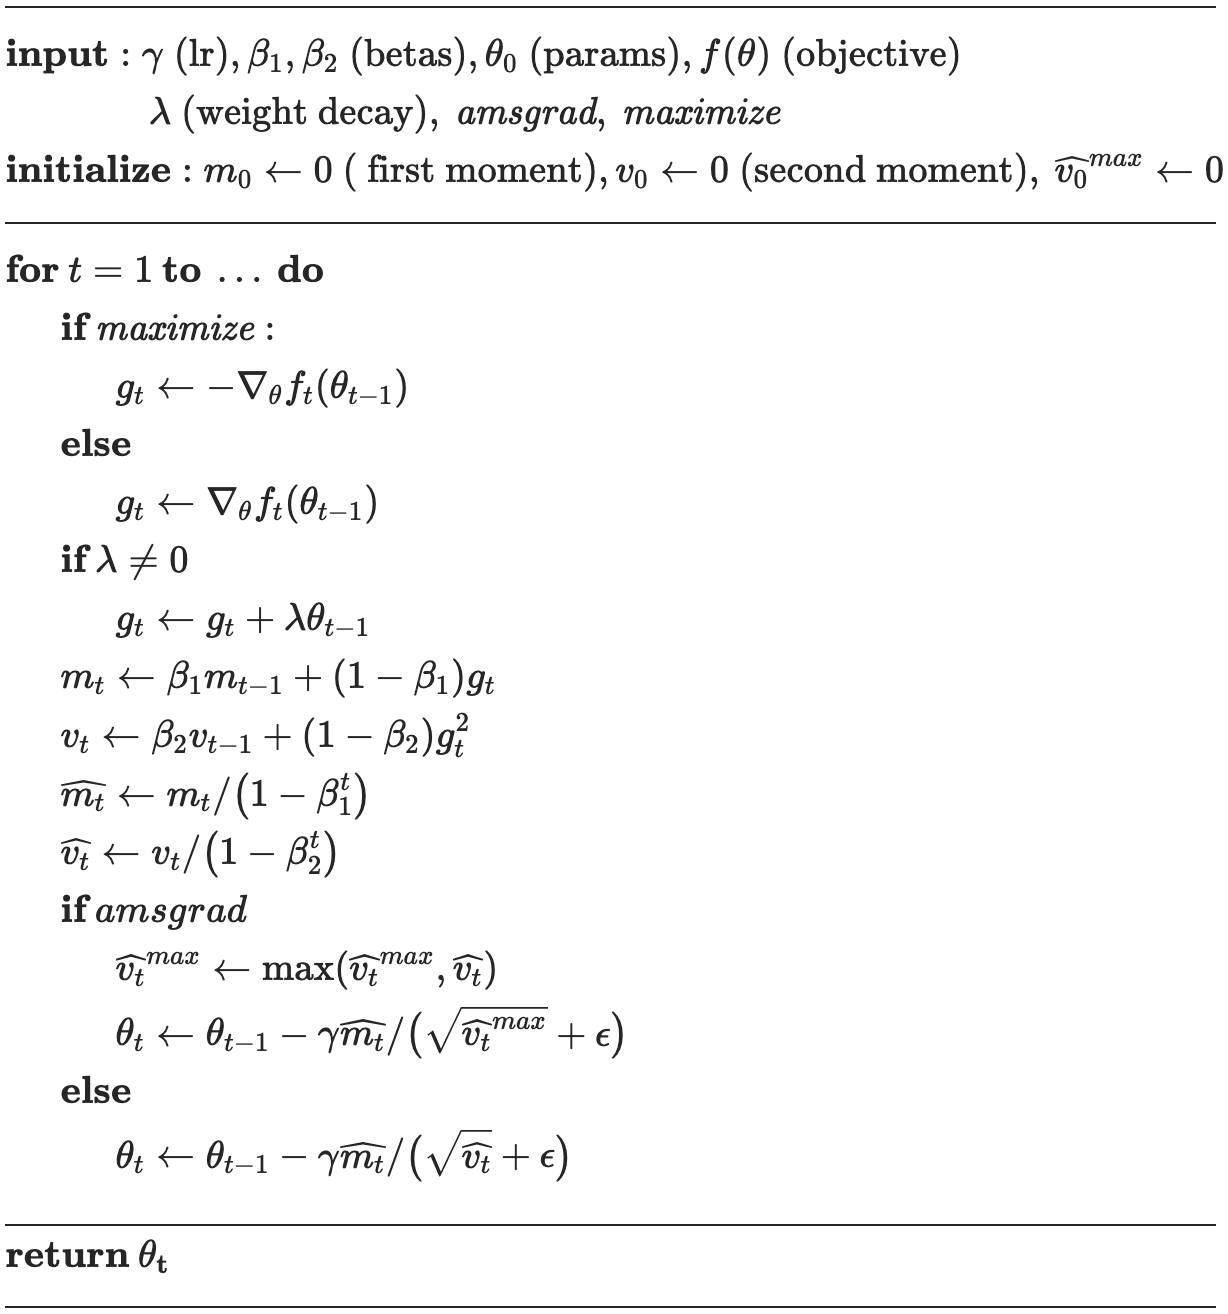
\includegraphics[scale=0.5]{img/adam.png}
		\caption{Pseudo code of Adam optimizer.}
		\label{adam}
	\end{figure}

\section{Loss function}
\indent
    \textbf{Cross entropy} (See Equation \ref{cross-entropy}) is used in this experiment, and it is also mostly used for classification tasks.
    \begin{equation}
        L(y, \hat{y}) = -[y\log\hat{y} + (1 - y)\log(1 - \hat{y})]
    \label{cross-entropy}
    \end{equation}
    where $y$ are ground truth labels and $\hat{y}$ are predicted labels.

\section{Data structure of linear layer}
\indent
    Data structure of linear layer is implemented using a class with only two member variables.
    It is well-defined, since \code{W} (weight matrix) and \code{b} (bias vector) are almost used at the same situations.
    \begin{lstlisting}[language=Python, caption={Date structure code of linear layer.}, label={linear-layer}]
    class Linear(object):      
        def __init__(self, W: np.ndarray, b: np.ndarray) -> None:
            self._W = W
            self._b = b
            
        @property
        def W(self) -> np.ndarray:
            return self._W
        
        @property
        def b(self) -> np.ndarray:
            return self._b
        
        @W.setter
        def W(self, W: np.ndarray) -> None:
            self._W = W
            
        @b.setter
        def b(self, b: np.ndarray) -> None:
            self._b = b
            
        def __str__(self) -> str:
            return f'<Linear W: {self._W.shape} b: {self._b.shape}>'\end{lstlisting}

	\chapter{Experimental results}
\indent
	PSNR on testing set is \textbf{25.79928}. \\
	Experiments of this chapter are done with setup below: 
	\begin{itemize}
		\item Seed: 42.
		\item Batch size: 64.
		\item Number of epochs and iterations: 100 / 600.
		\item Learning rate: $2 \times 10^{-3}$.
		\item Optimizer: \code{Adam} with betas (0.9, 0.999).
		\item RNN hidden size: 256.
		\item Number of hidden layers: 2 (predictor) / 1 (prior).
		\item RNN input and output size: 64 / 128.
	\end{itemize} 

\section{Video prediction on testing set}
	\begin{figure}[H]
		\centering
		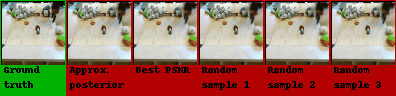
\includegraphics[scale=0.9]{img/test_pred-2.png}
		\caption{Samples from testing set (only 3rd frame is displayed here, details are in Appendix \ref{more-results}).}
		\label{test-prediction}
	\end{figure}

\section{KL loss and PSNR curves}
	From Figures \ref{result-mono} and \ref{result-cyc}, 
	we can see that I set the teacher-forcing ratio to fixed 1 during entire training, 
	and training loss decreases smoothly and PSNR increases fast under both monotonic and cyclical modes. 
	The unstable PSNR is partially due to the validation PSNR is tested each 5 epochs, 
	if we test it each epoch, the curve will be much more smooth. \\
	From my experiments, results of two modes seem similar, both for loss and PSNR.
	Also, the testing PSNR is similar to best validation PSNR, and even higher, i.e., 
	testing PSNR is \textbf{25.79928}, best validation PSNR for monotonic mode is \textbf{25.73145}, 
	and best validation PSNR for cyclical mode is \textbf{25.76462}.
	Exposure bias seems not occur during training with fixed teacher-forcing ratio 1.
	
	\begin{figure}[H]
		\centering
		\begin{subfigure}
			\centering
			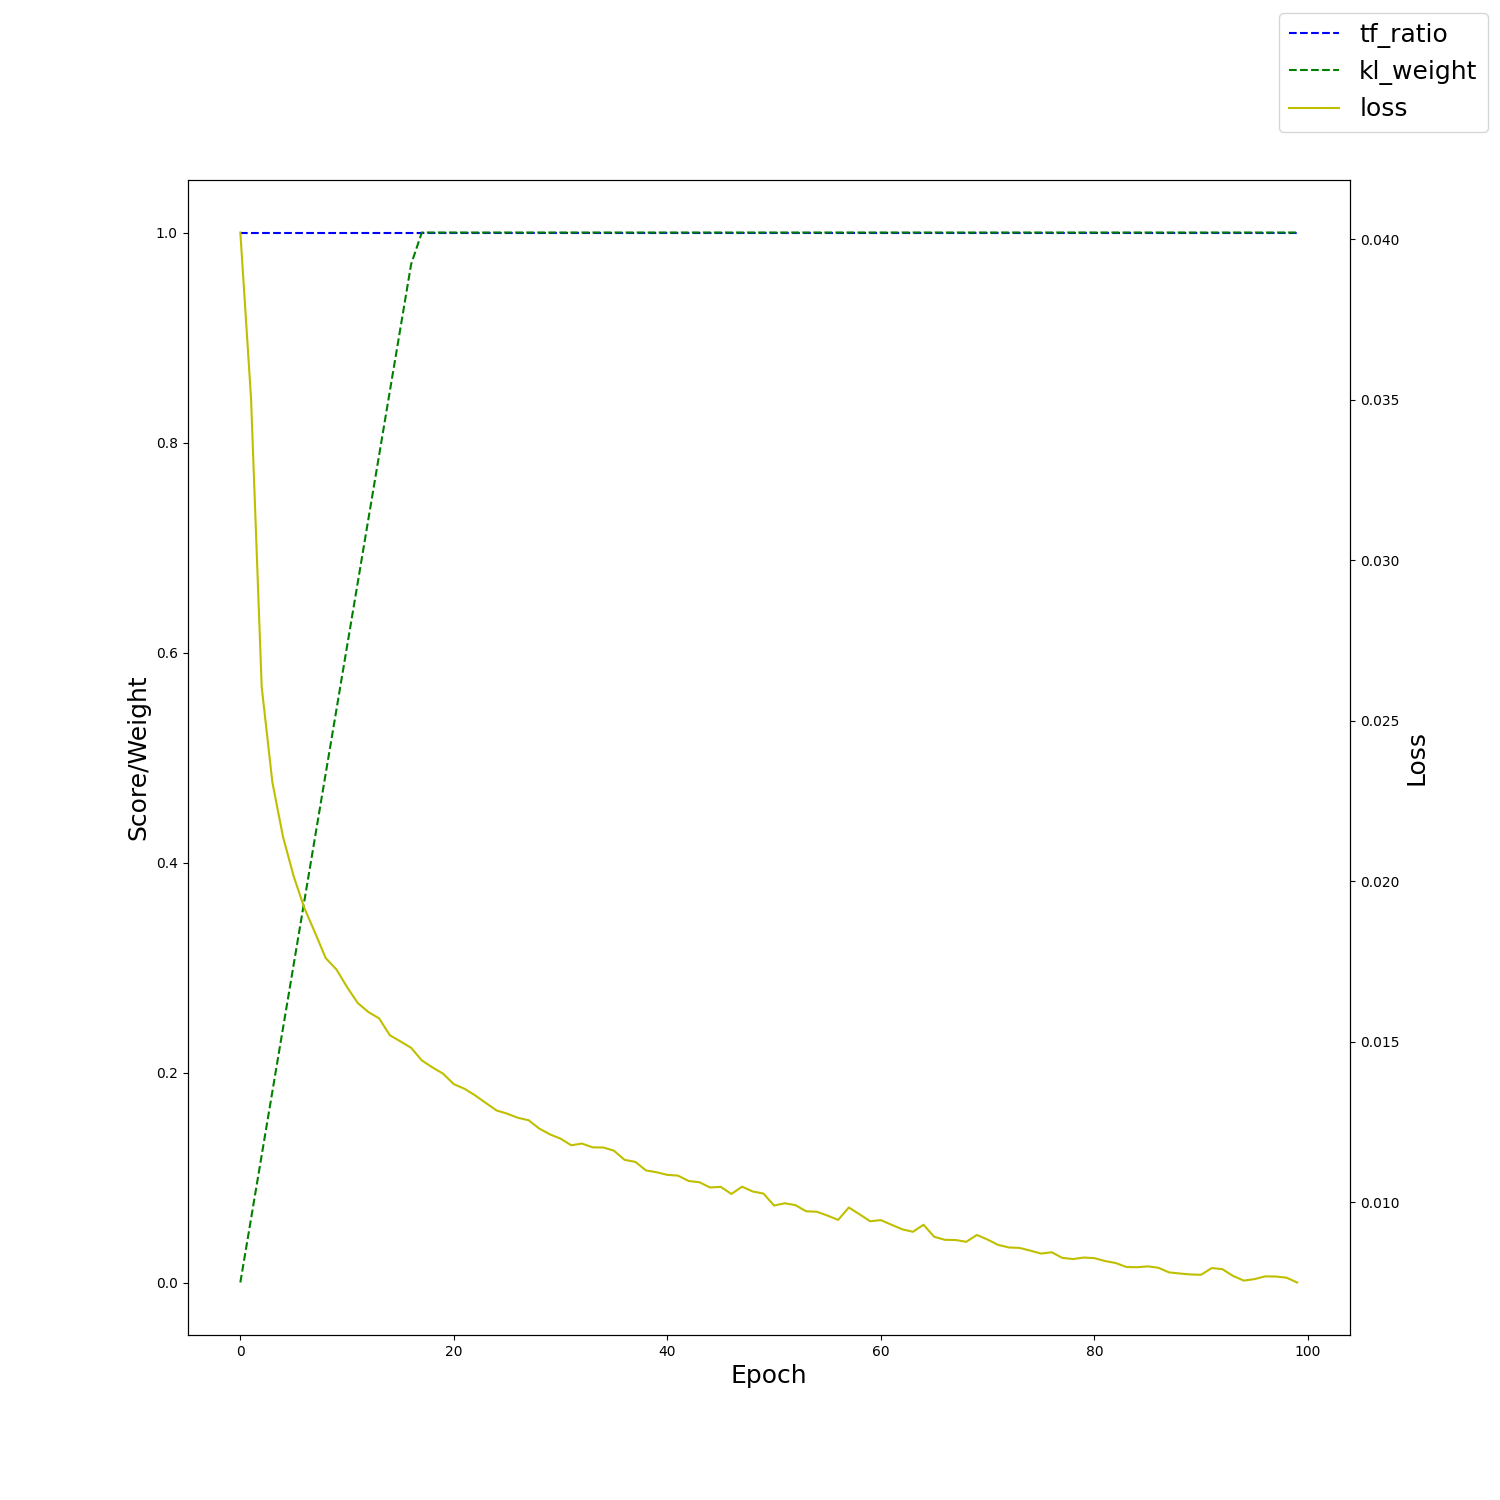
\includegraphics[width=0.45\textwidth]{img/loss_mono.png}
			\label{loss-mono}
		\end{subfigure}
		\hfill
		\begin{subfigure}
			\centering
			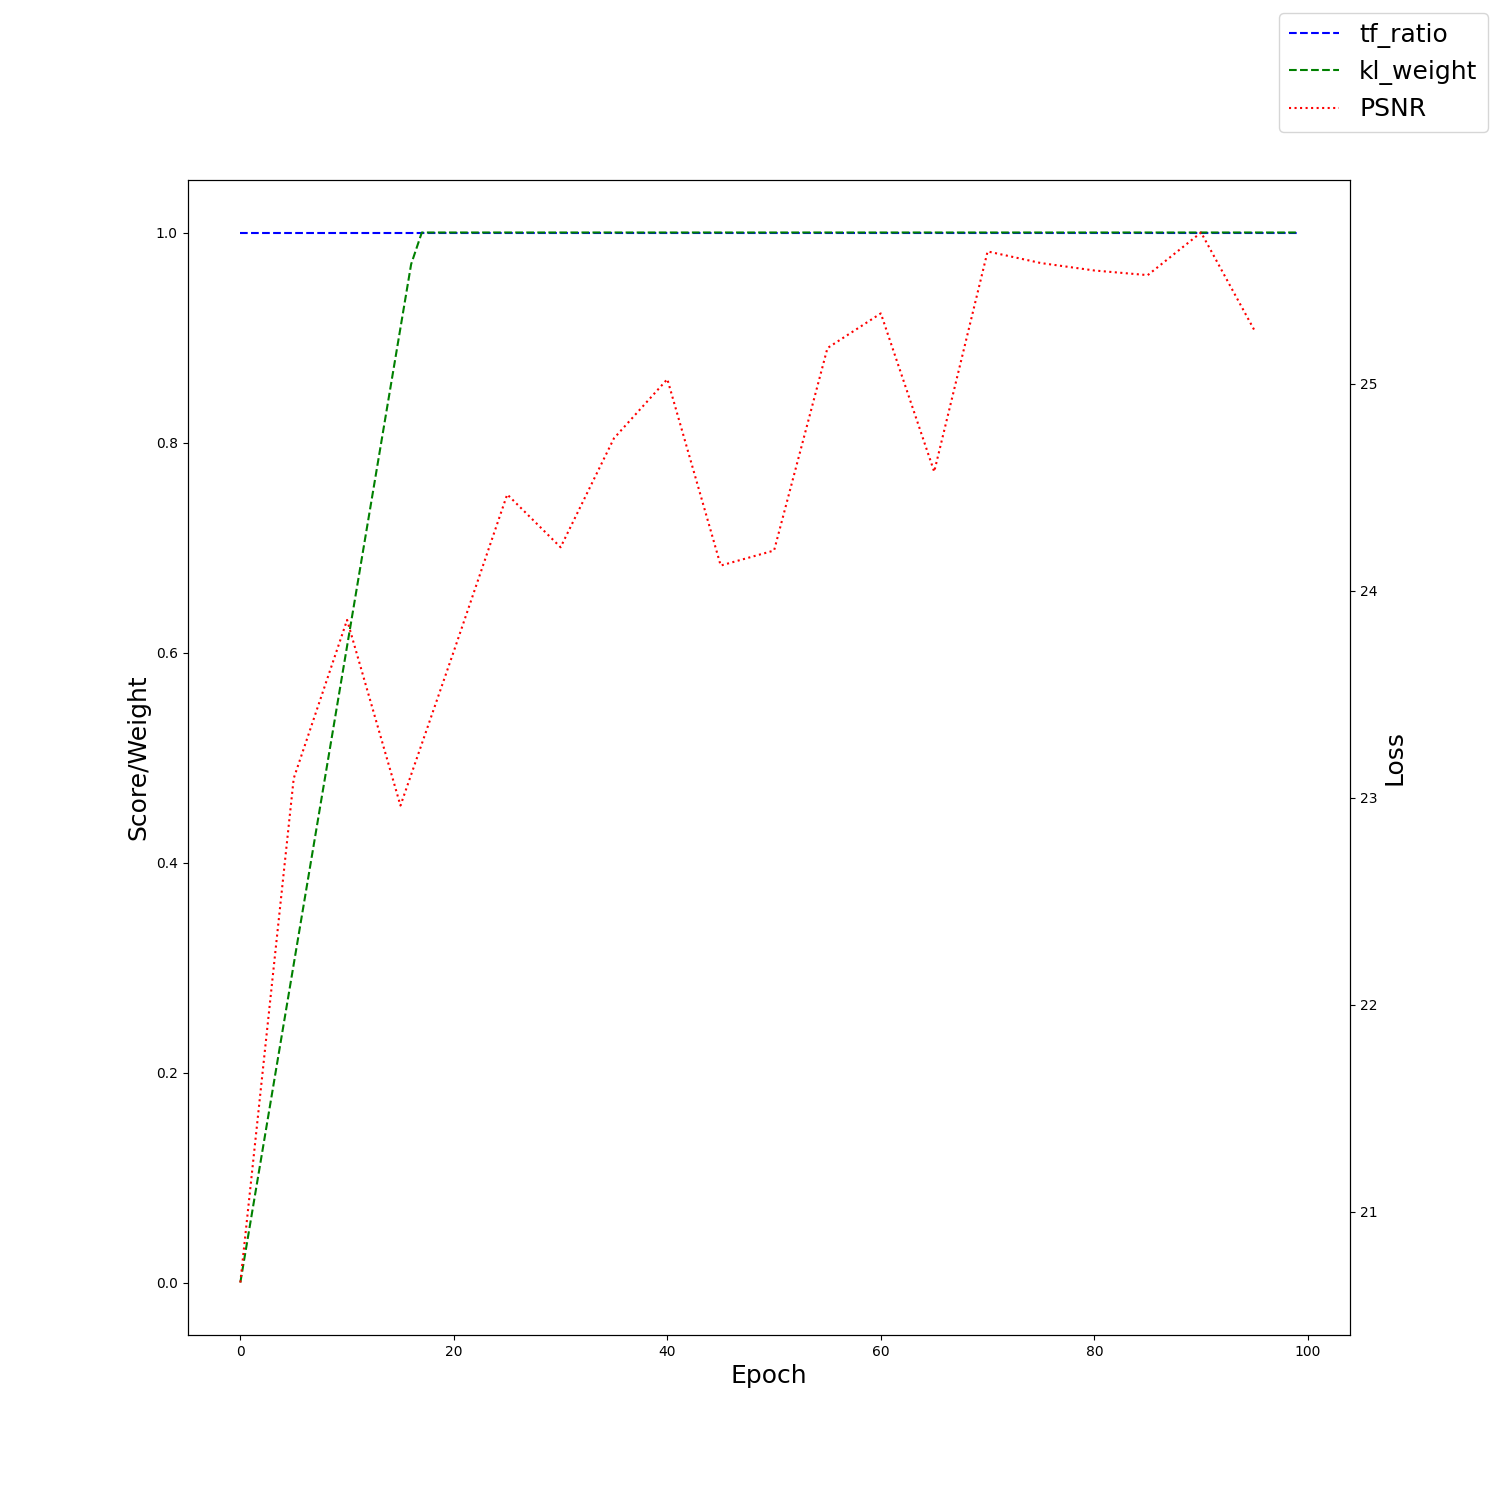
\includegraphics[width=0.45\textwidth]{img/psnr_mono.png}
			\label{psnr-mono}
		\end{subfigure}
		\hfill
		\caption{KL loss and PSNR of \textbf{monotonic} KL annealing mode.}
		\label{result-mono}
	\end{figure}

	\begin{figure}[H]
		\centering
		\begin{subfigure}
			\centering
			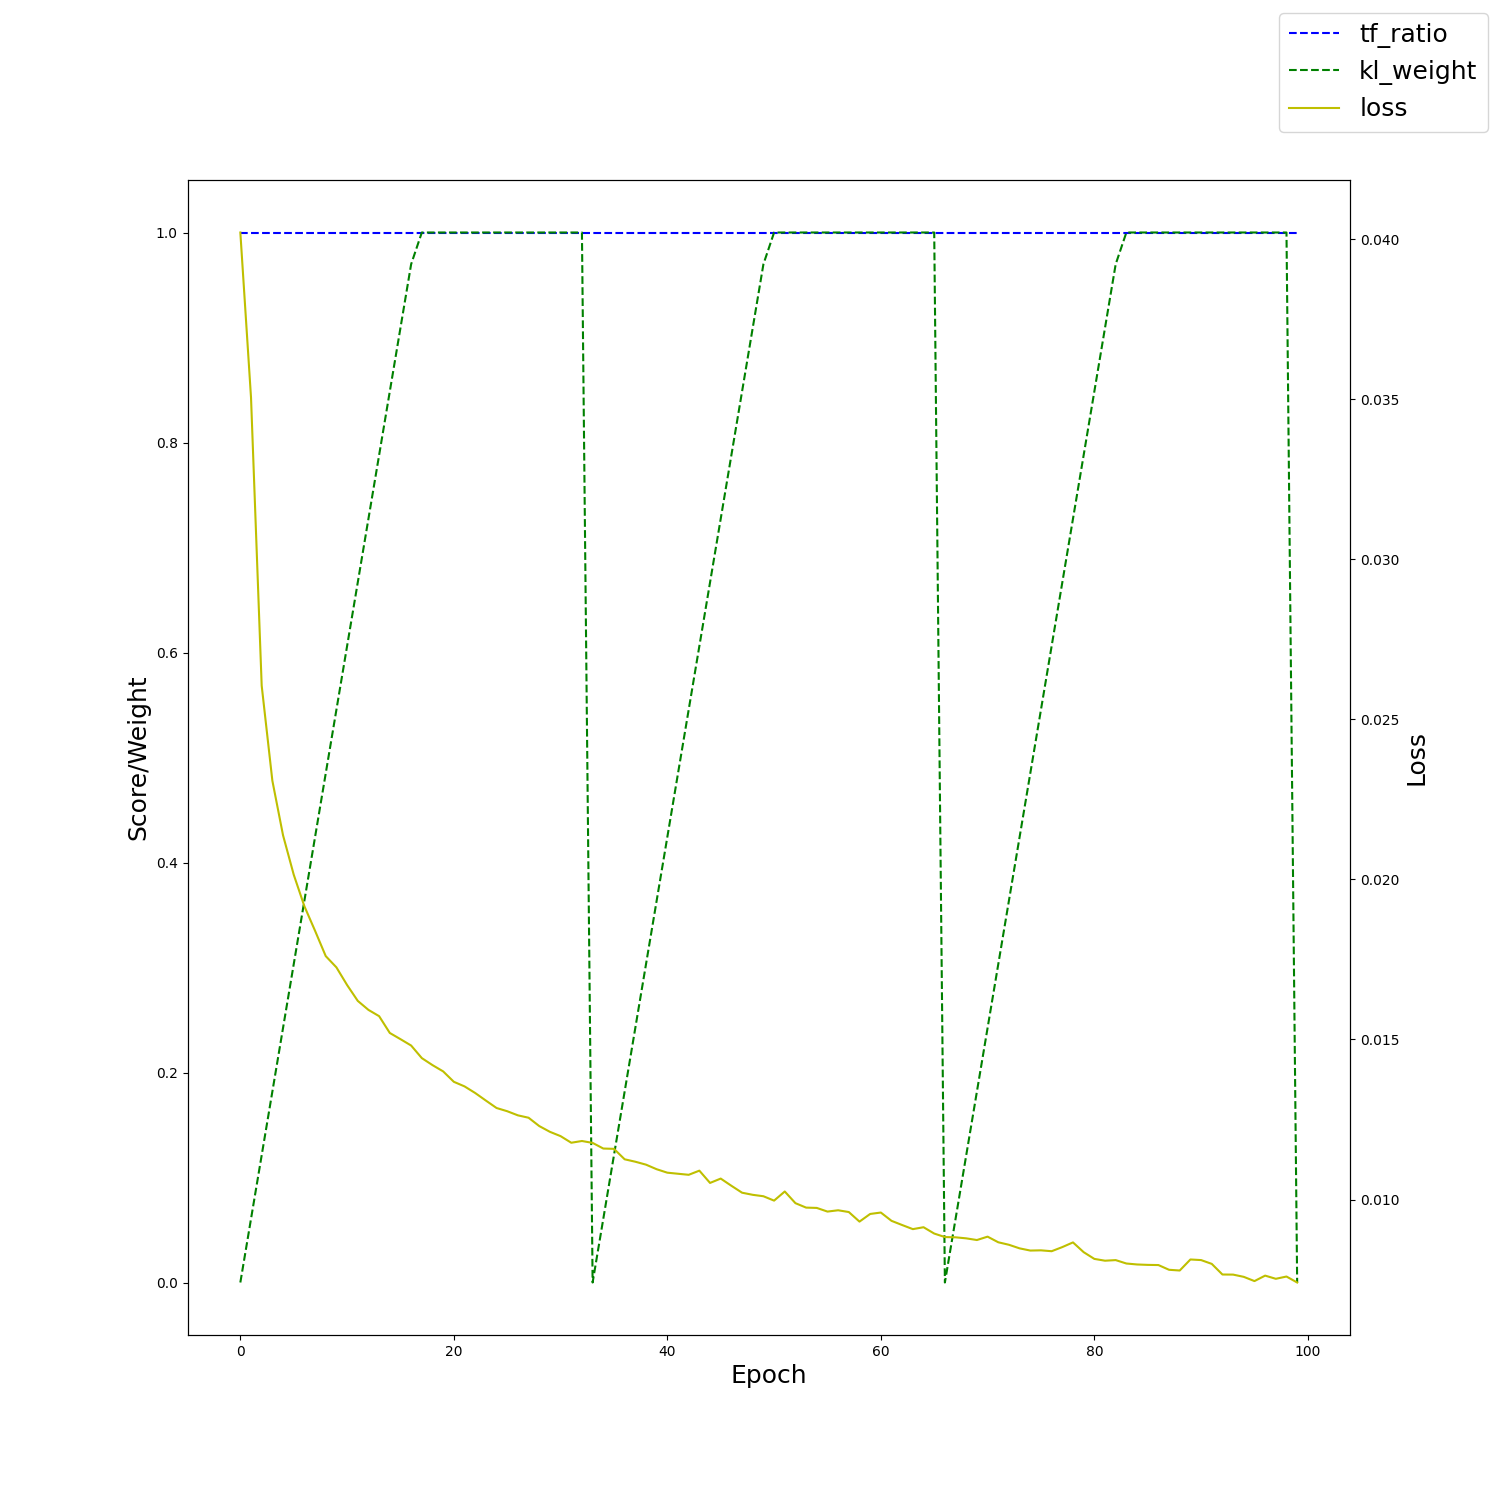
\includegraphics[width=0.45\textwidth]{img/loss_cyc.png}
			\label{loss-cyc}
		\end{subfigure}
		\hfill
		\begin{subfigure}
			\centering
			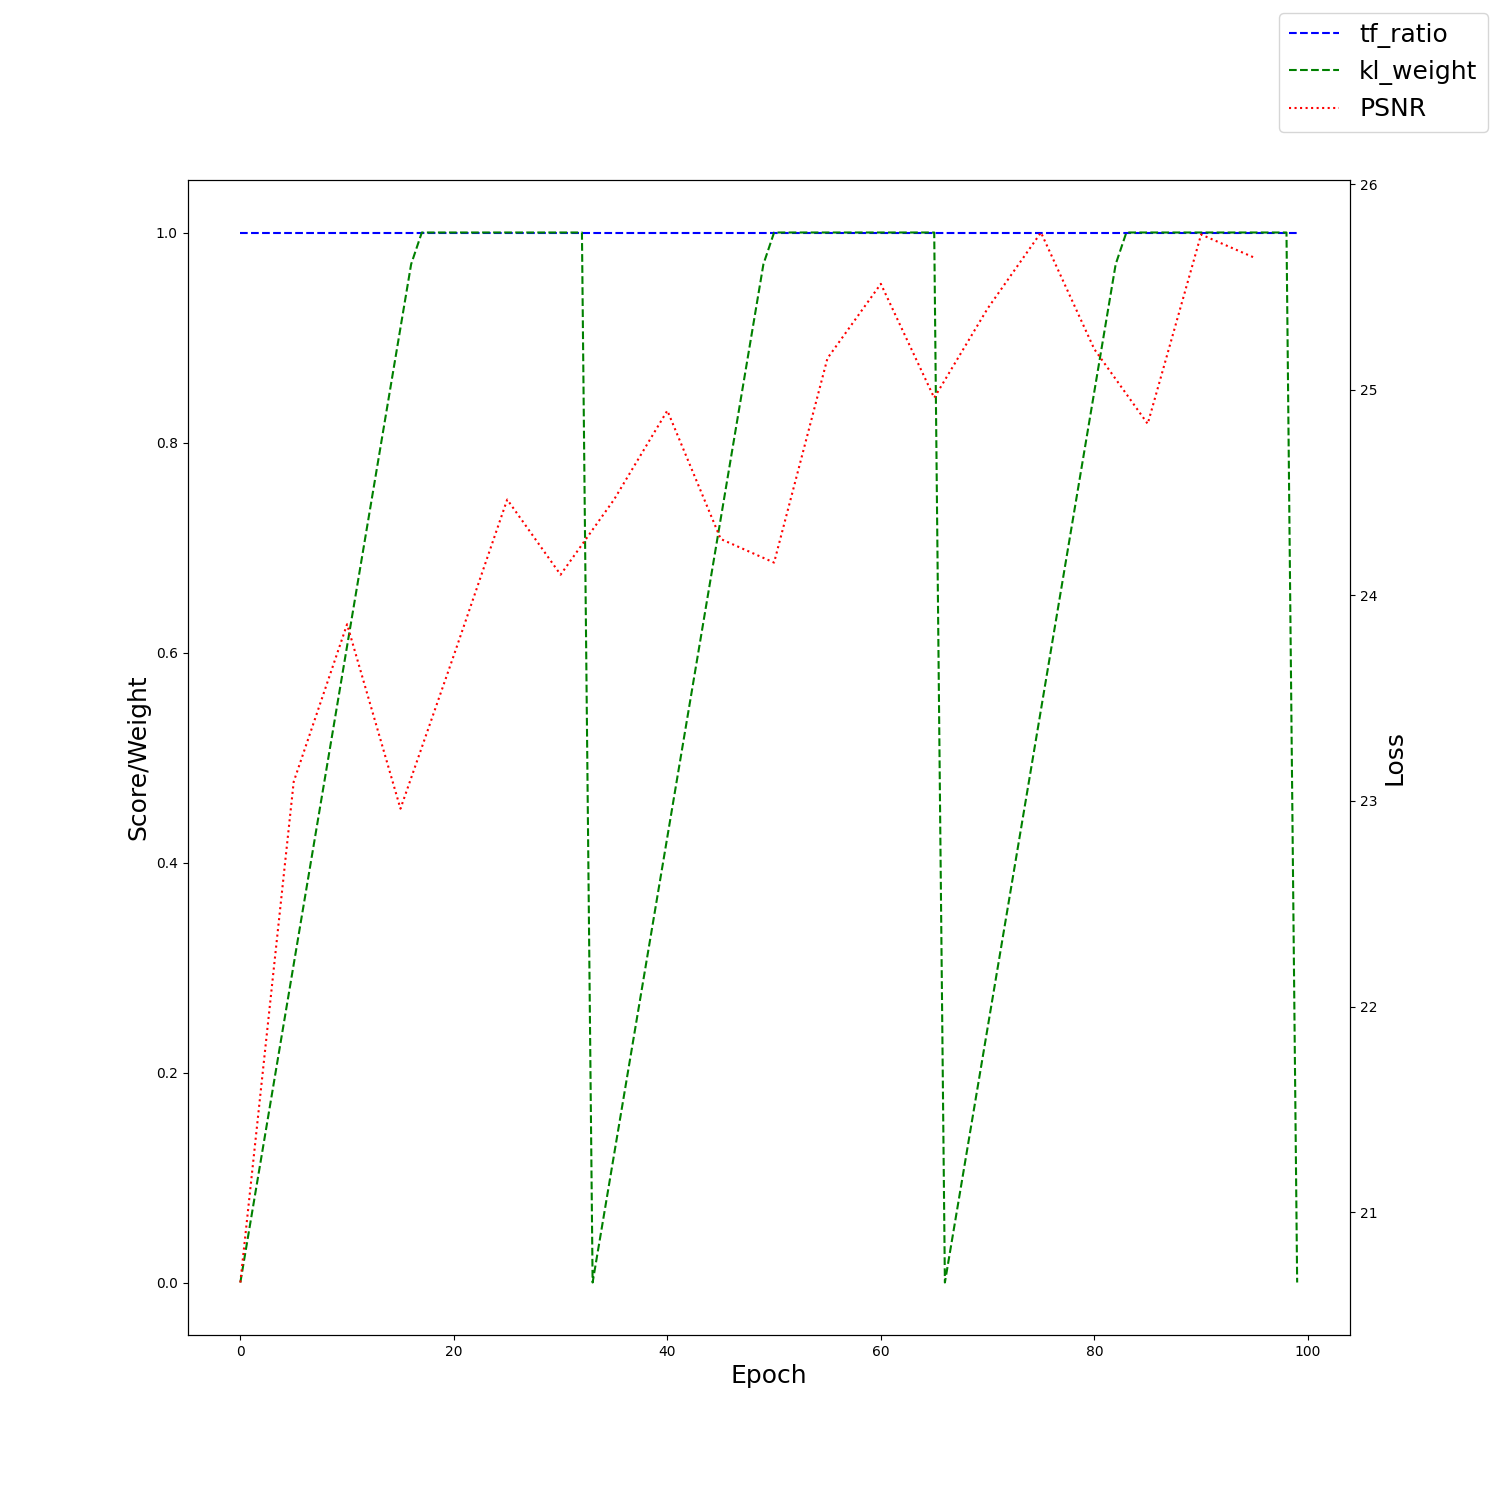
\includegraphics[width=0.45\textwidth]{img/psnr_cyc.png}
			\label{psnr-cyc}
		\end{subfigure}
		\hfill
		\caption{KL loss and PSNR of \textbf{cyclical} KL annealing mode.}
		\label{result-cyc}
	\end{figure}

	\chapter{Conclusion}
\indent
	After this experiment, I found that \textbf{patterns} play an important role in this task.\\
	With original 4 patterns, the average reached 2048-tile percentage is only about \textcolor{blue}{\textbf{90\%}} after 350K iterations training.
	However, with another 4 patterns, totally 8 patterns are used, it reaches about \textcolor{blue}{\textbf{95\%}}.

	% \bibliographystyle{plain}
\bibliography{bibliography}
\addcontentsline{toc}{chapter}{\bibname}
	\begin{appendices}
		\chapter{More results}
\subsection{EEGNet}\label{results-eegnet}
	\begin{figure}[H]
		\centering
		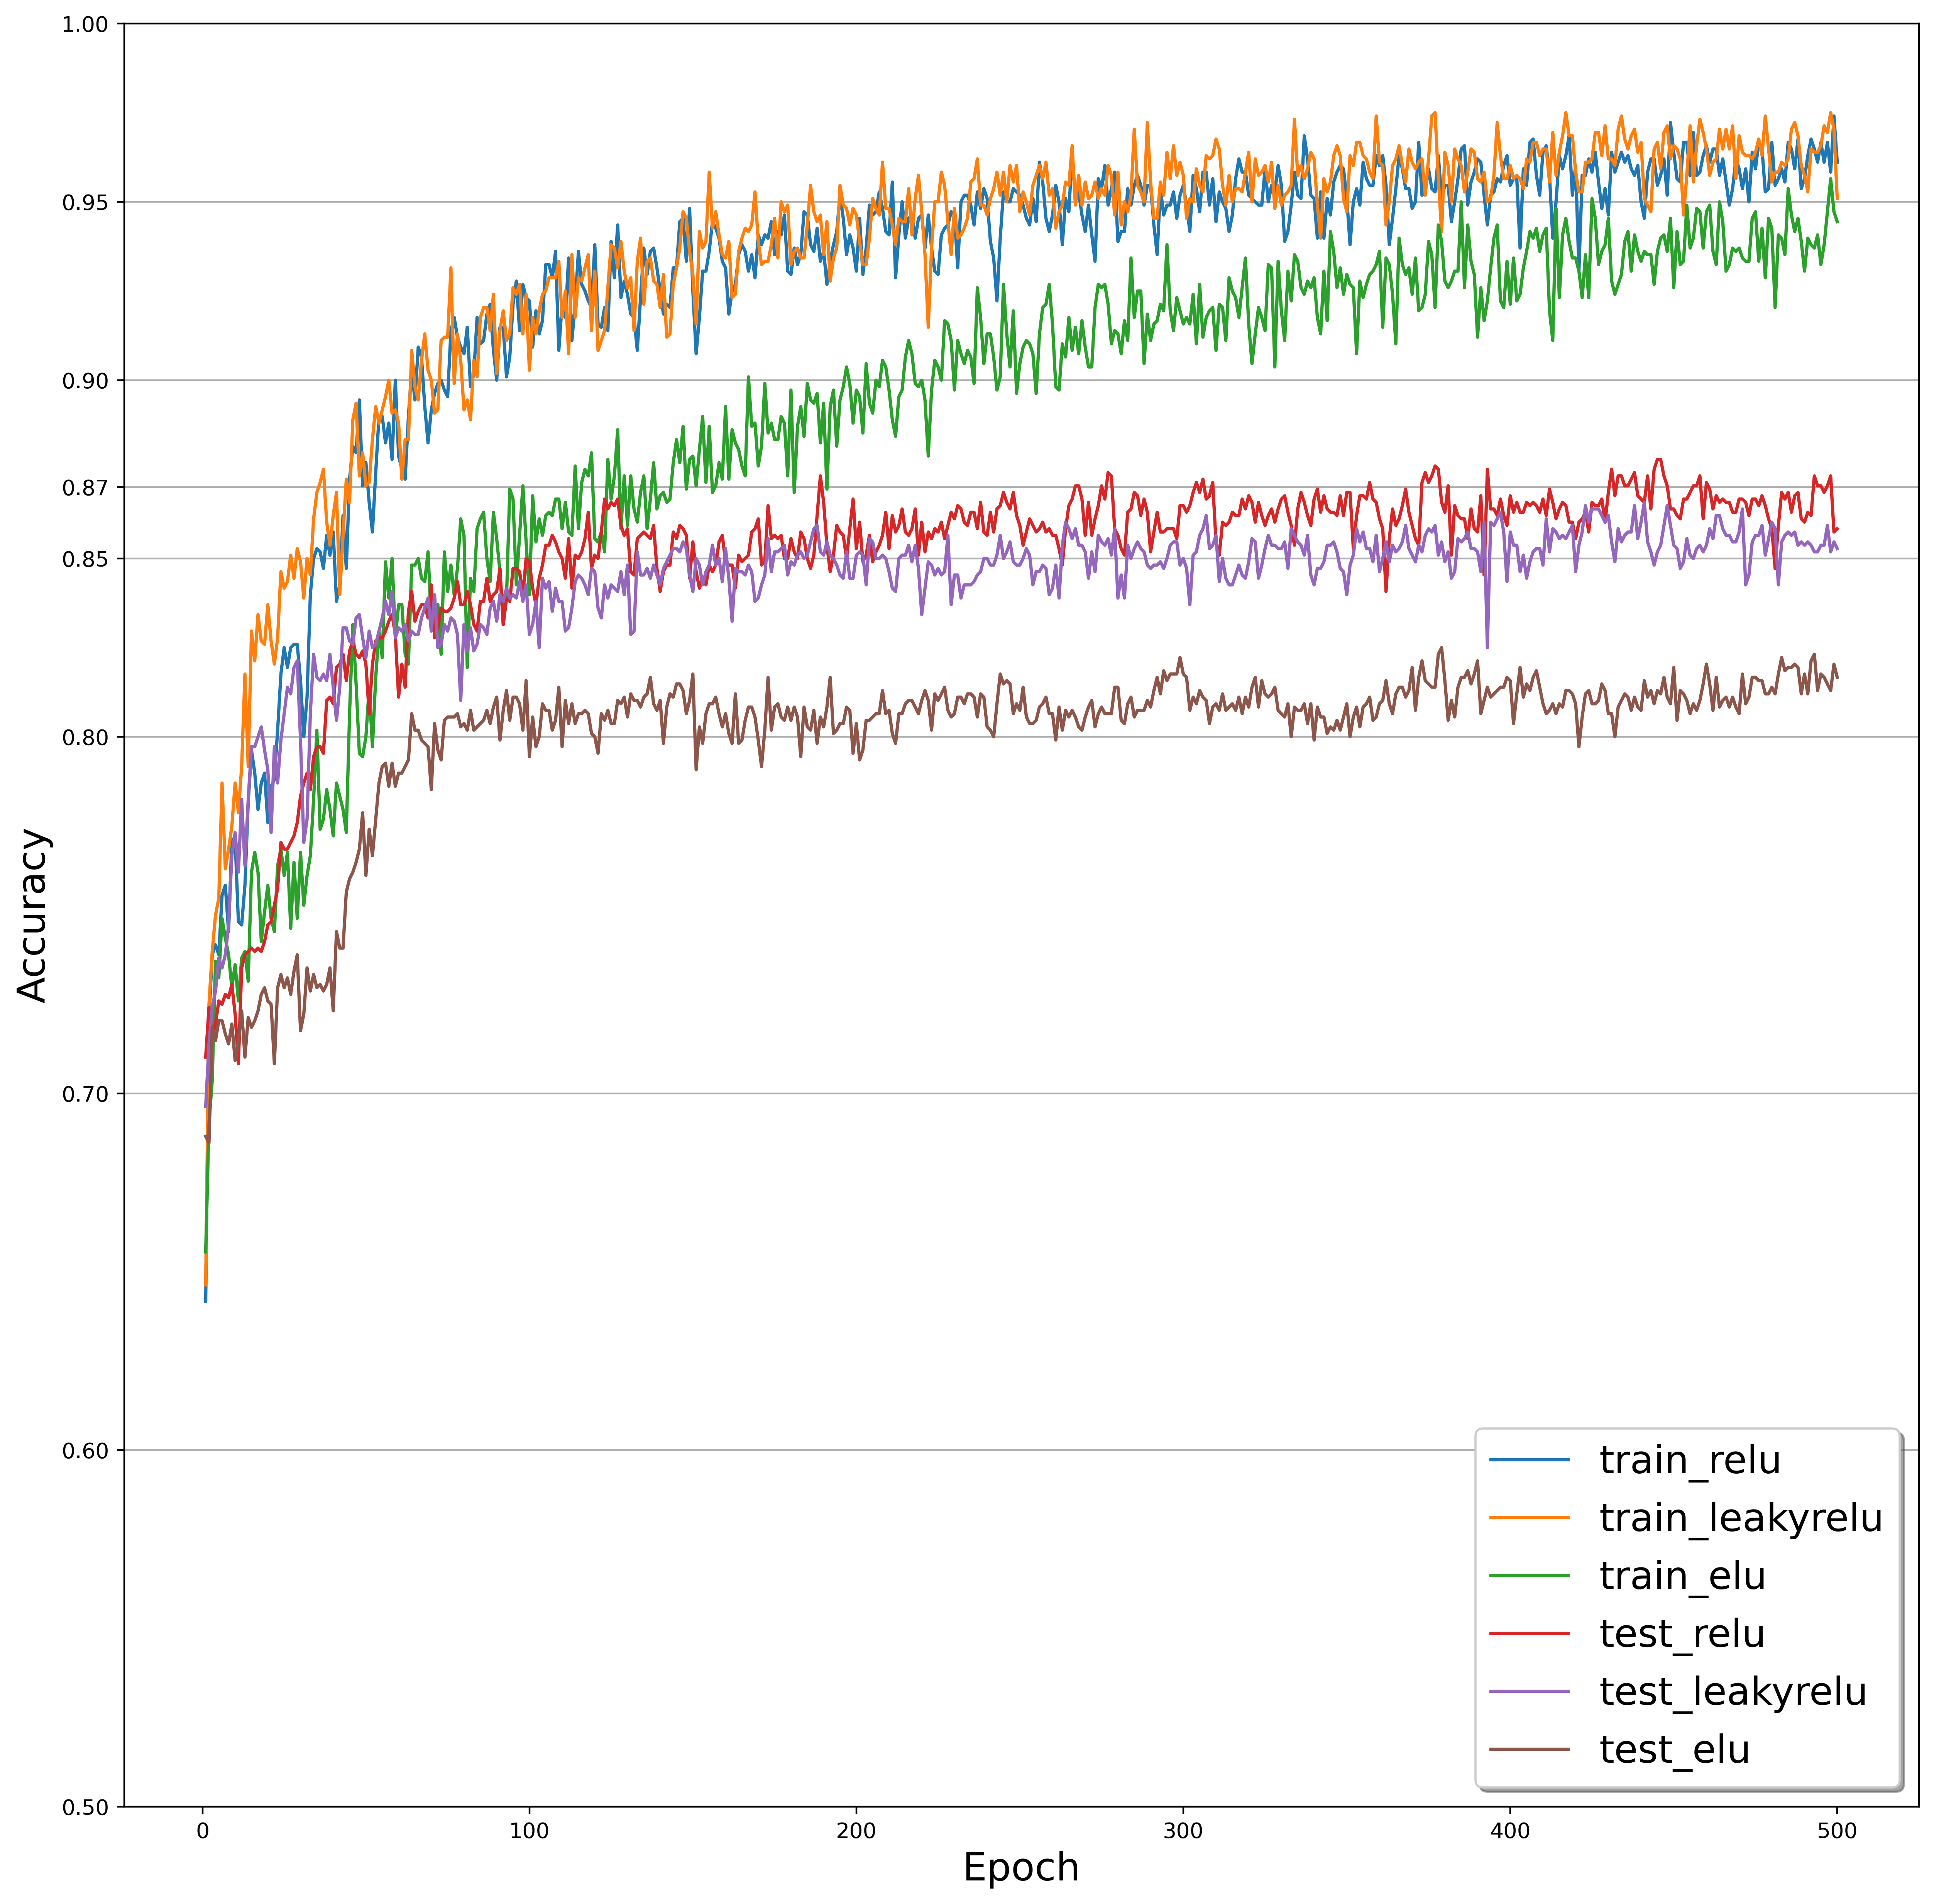
\includegraphics[width=0.45\textwidth]{results/eegnet_adam_64_0.005_0.5_acc.png}
		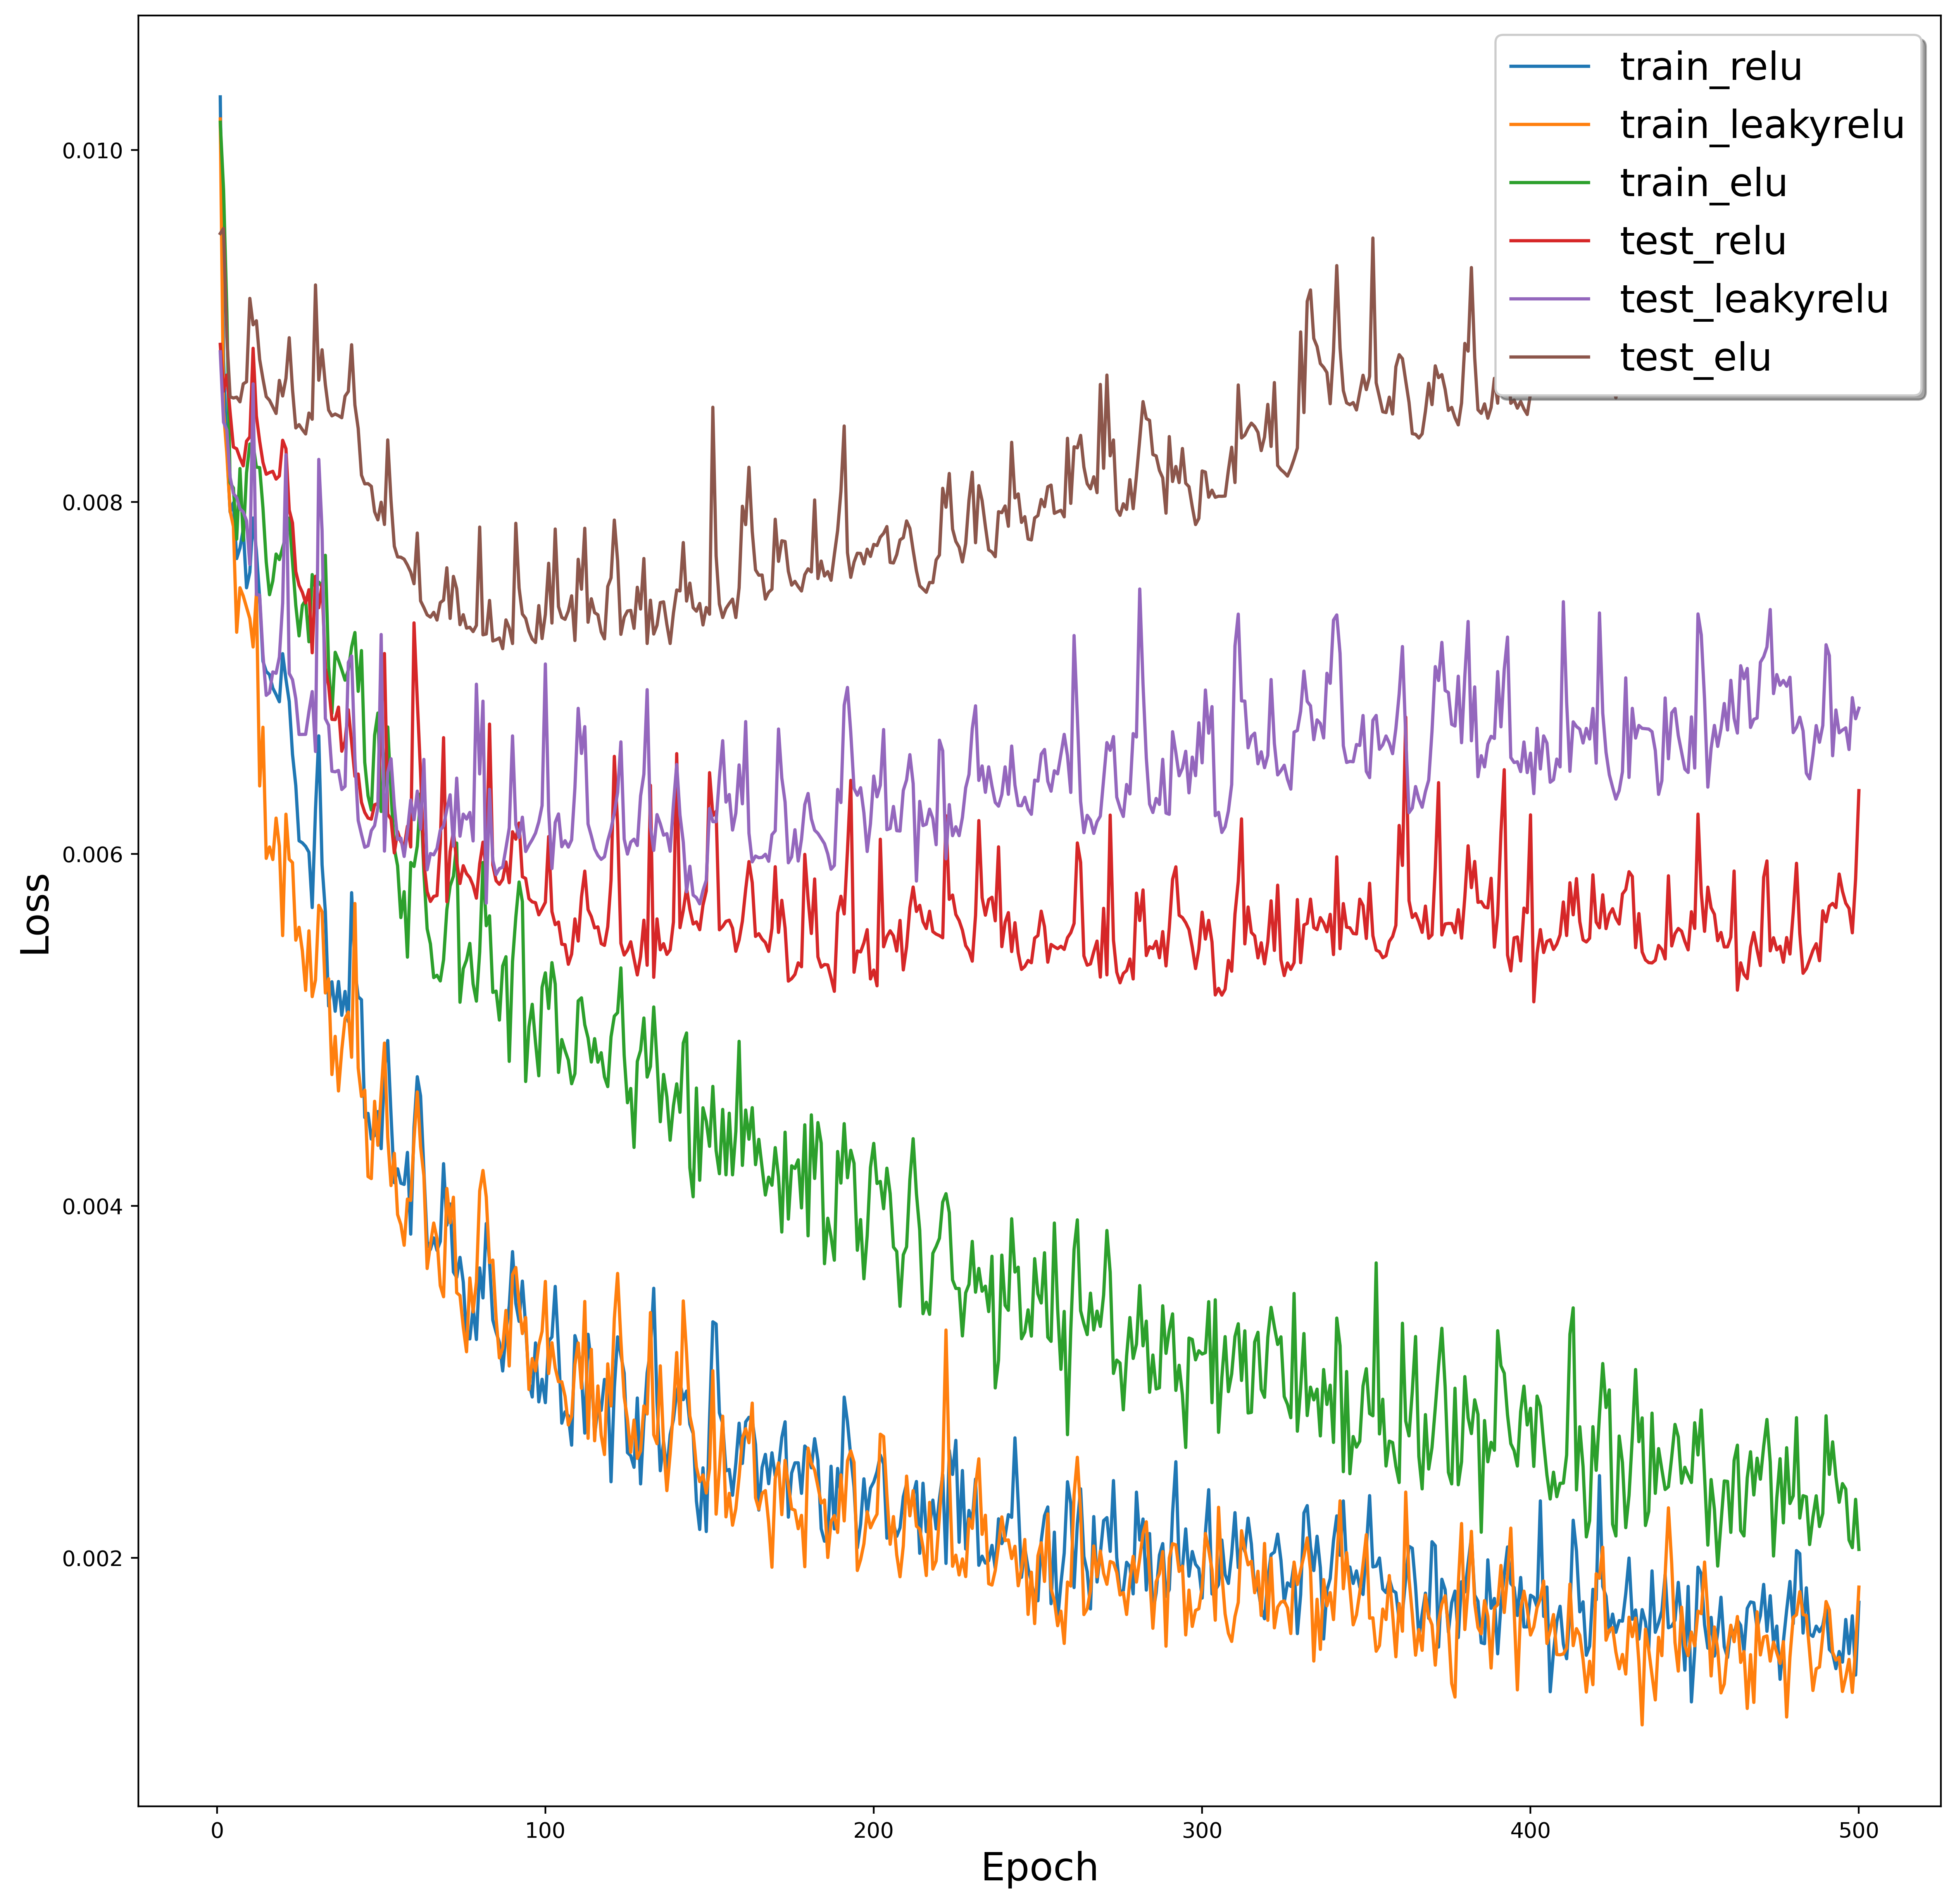
\includegraphics[width=0.45\textwidth]{results/eegnet_adam_64_0.005_0.5_loss.png}
		\caption{EEGNet with Adam, 64 batch size, \\ $5 \times 10^{-3}$ learning rate, and 50\% dropout.}
   	\end{figure}
	\begin{figure}[H]
		\centering
		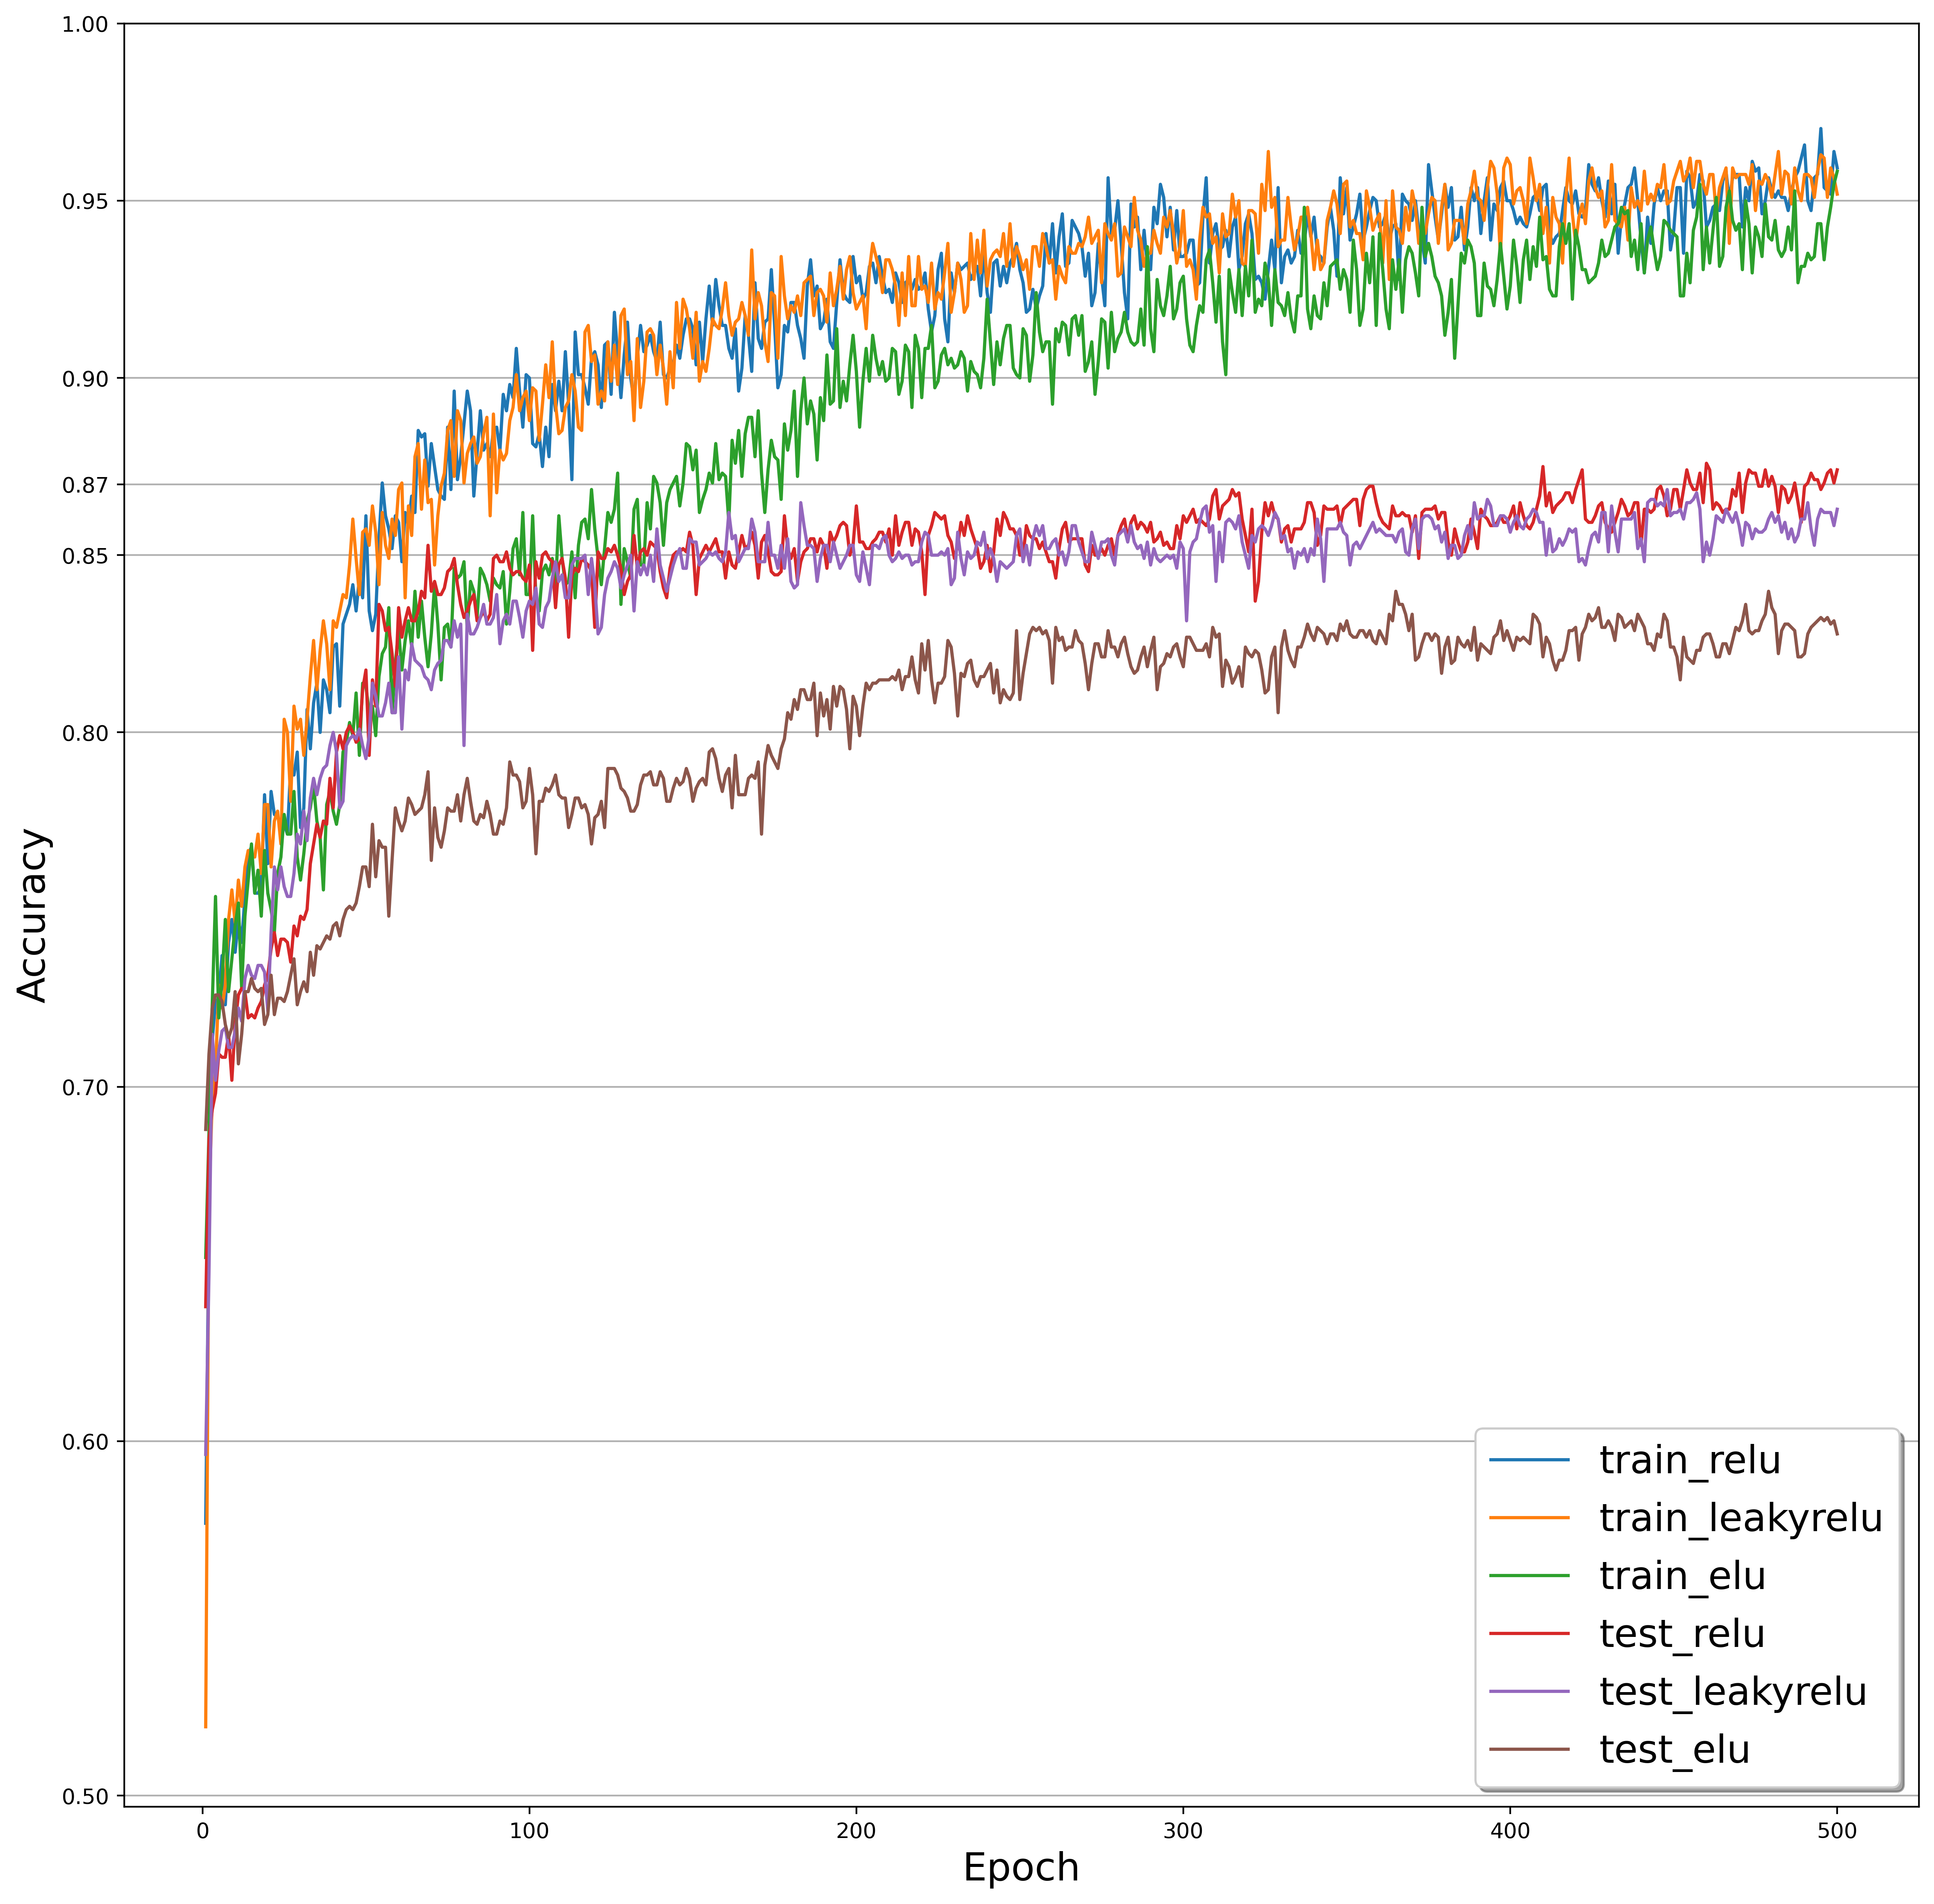
\includegraphics[width=0.45\textwidth]{results/eegnet_adam_256_0.005_0.5_acc.png}
		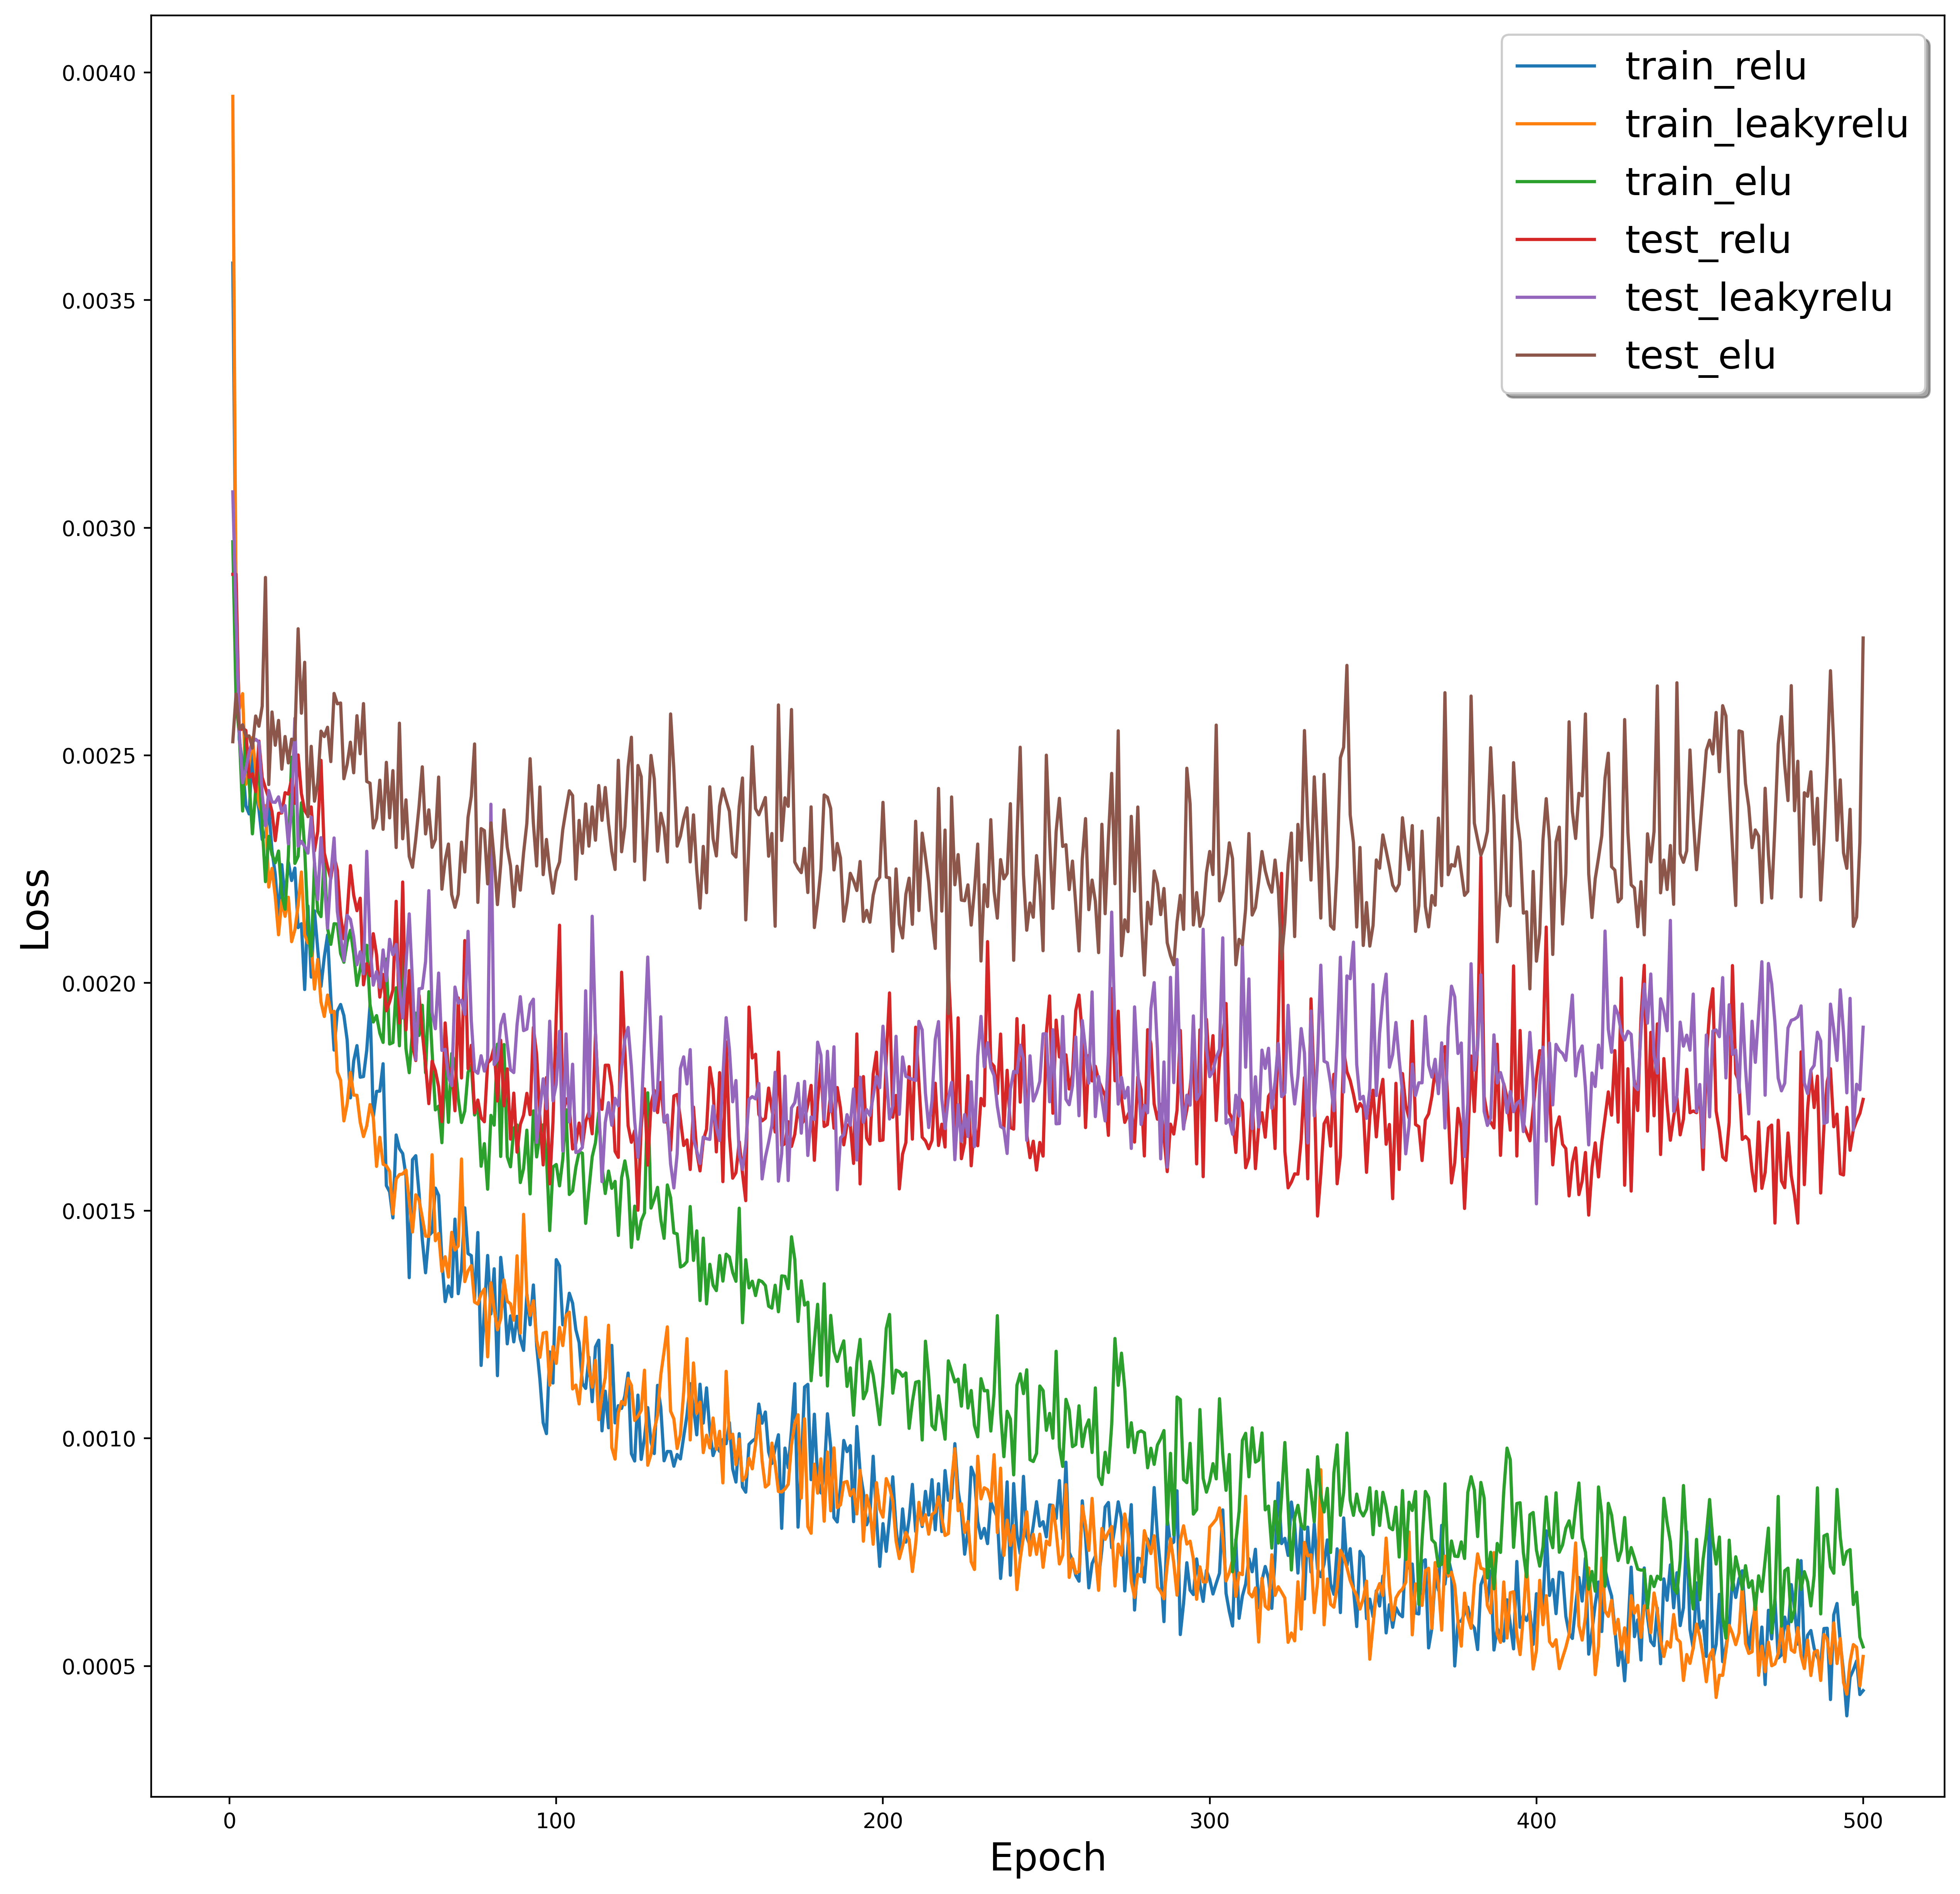
\includegraphics[width=0.45\textwidth]{results/eegnet_adam_256_0.005_0.5_loss.png}
		\caption{EEGNet with Adam, 256 batch size, \\ $5 \times 10^{-3}$ learning rate, and 50\% dropout.}
   	\end{figure}
	\begin{figure}[H]
		\centering
		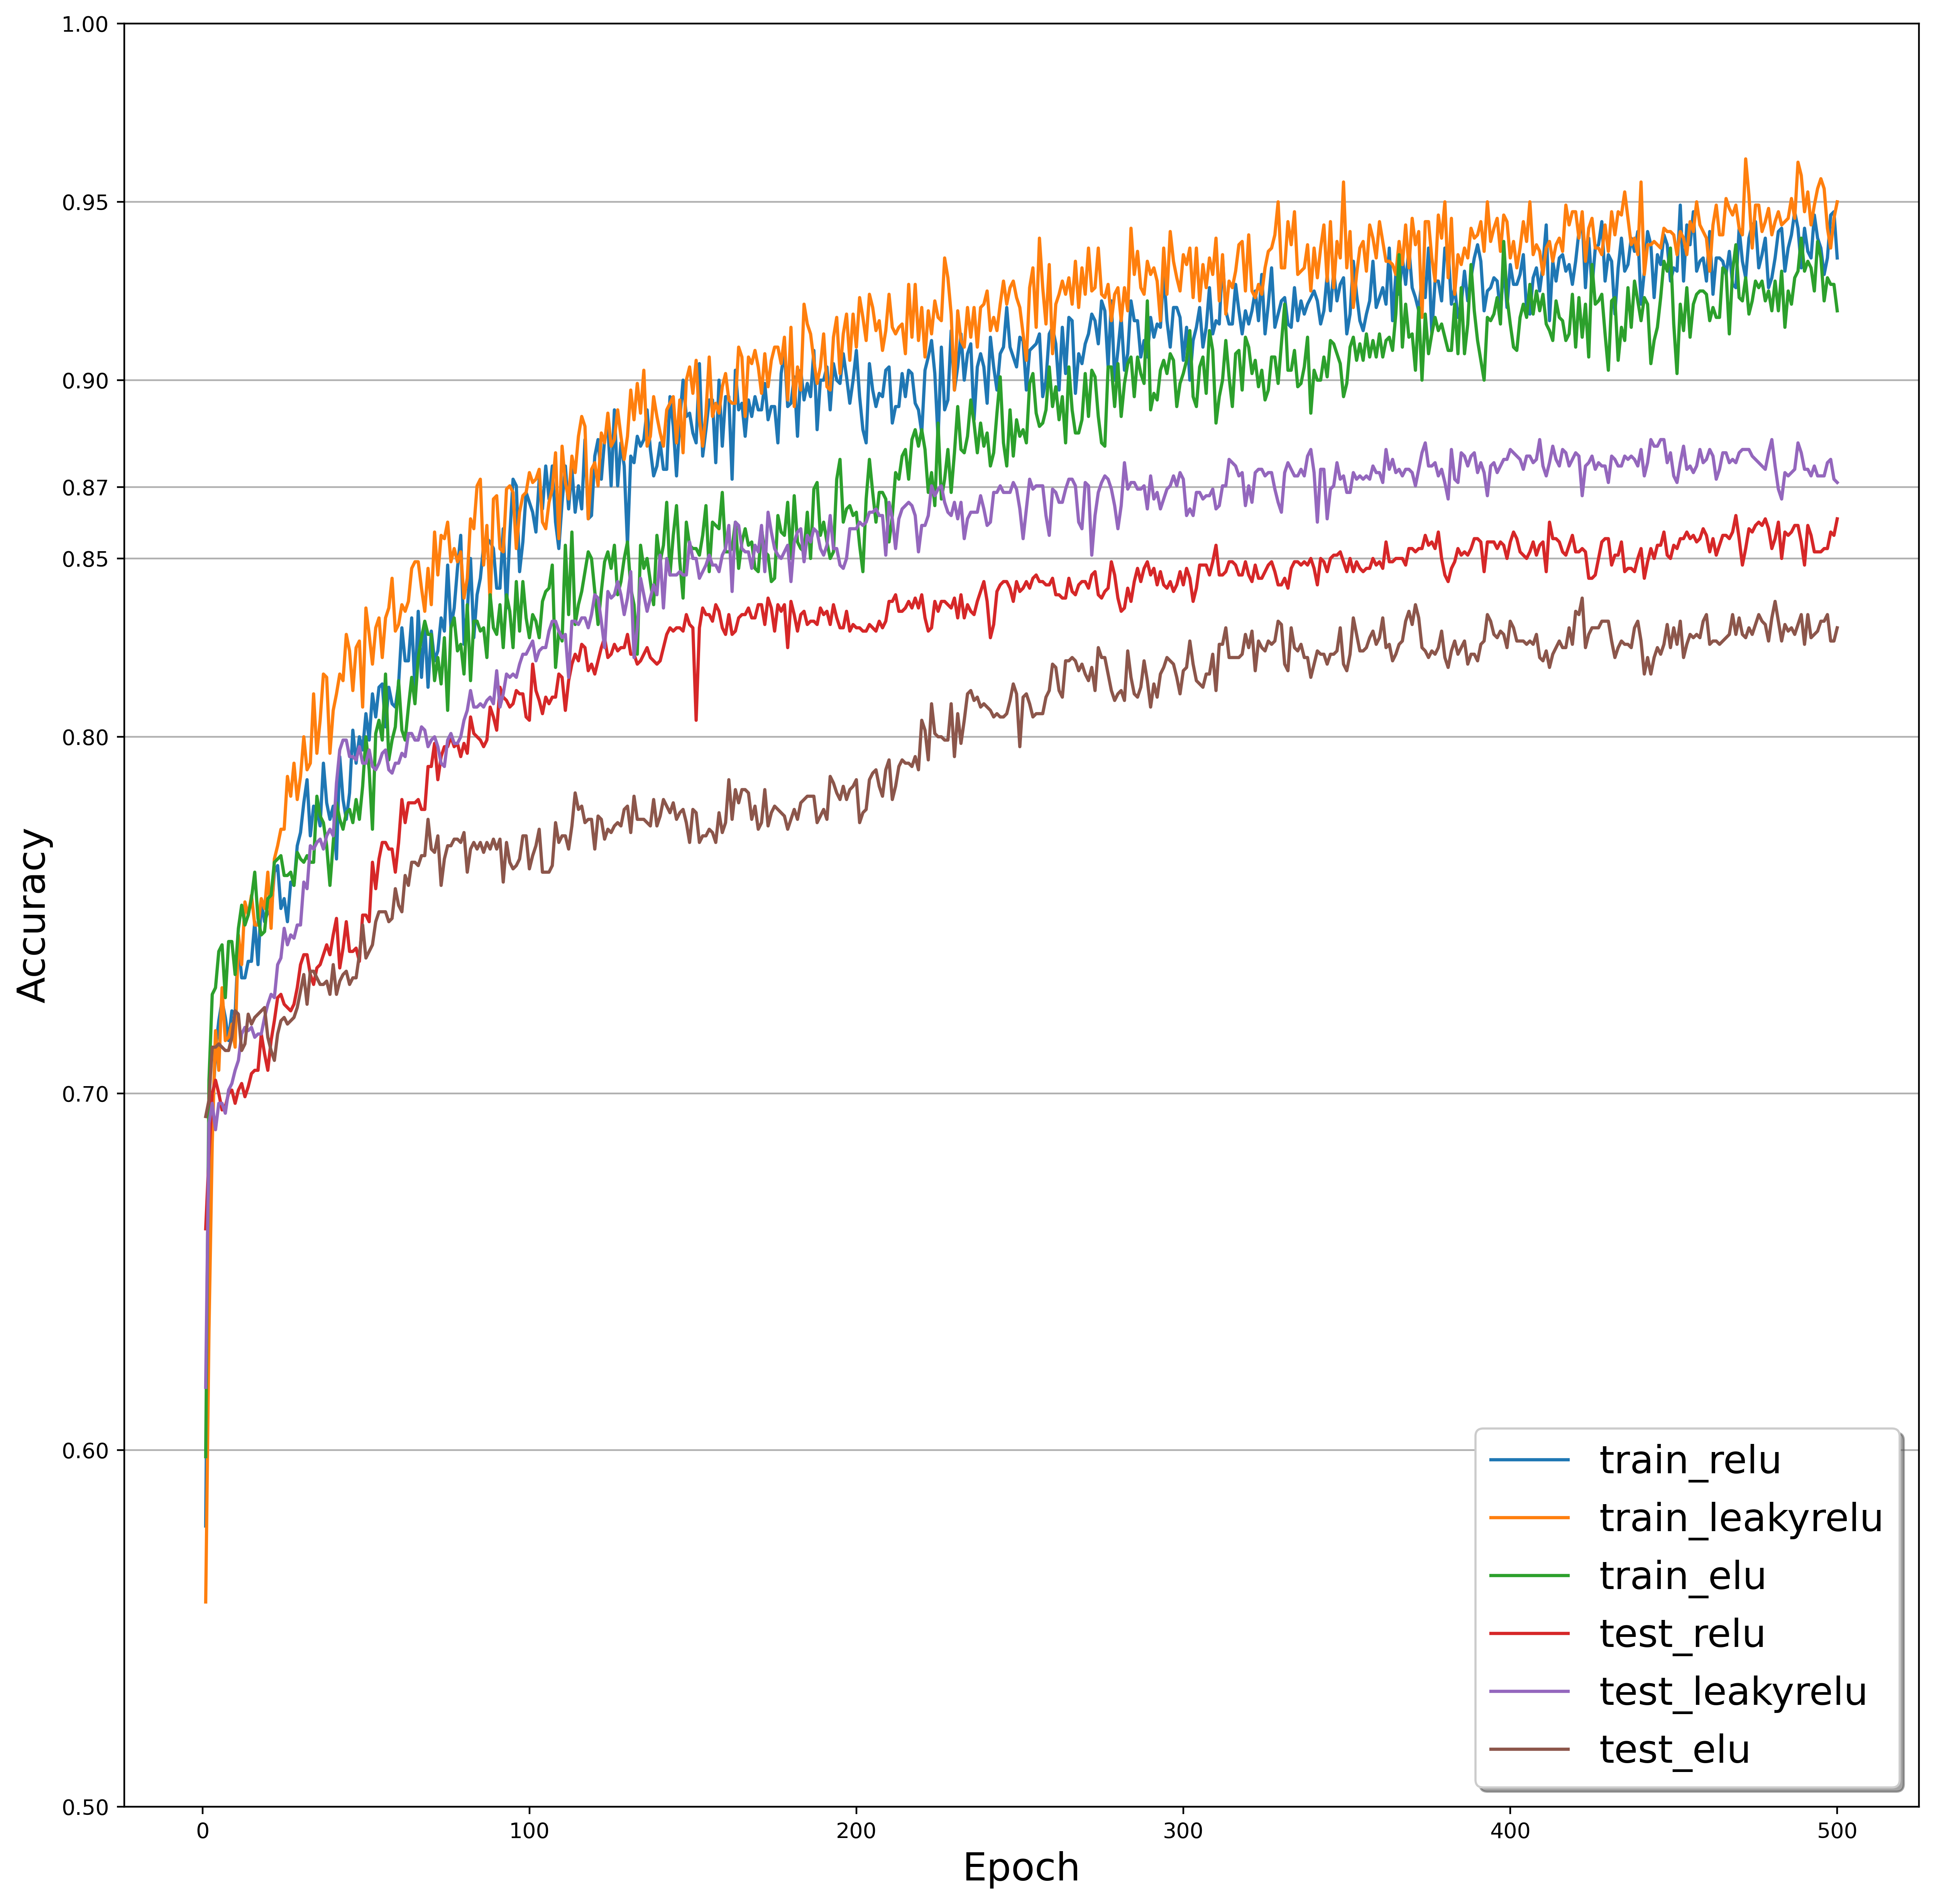
\includegraphics[width=0.45\textwidth]{results/eegnet_adam_128_0.001_0.5_acc.png}
		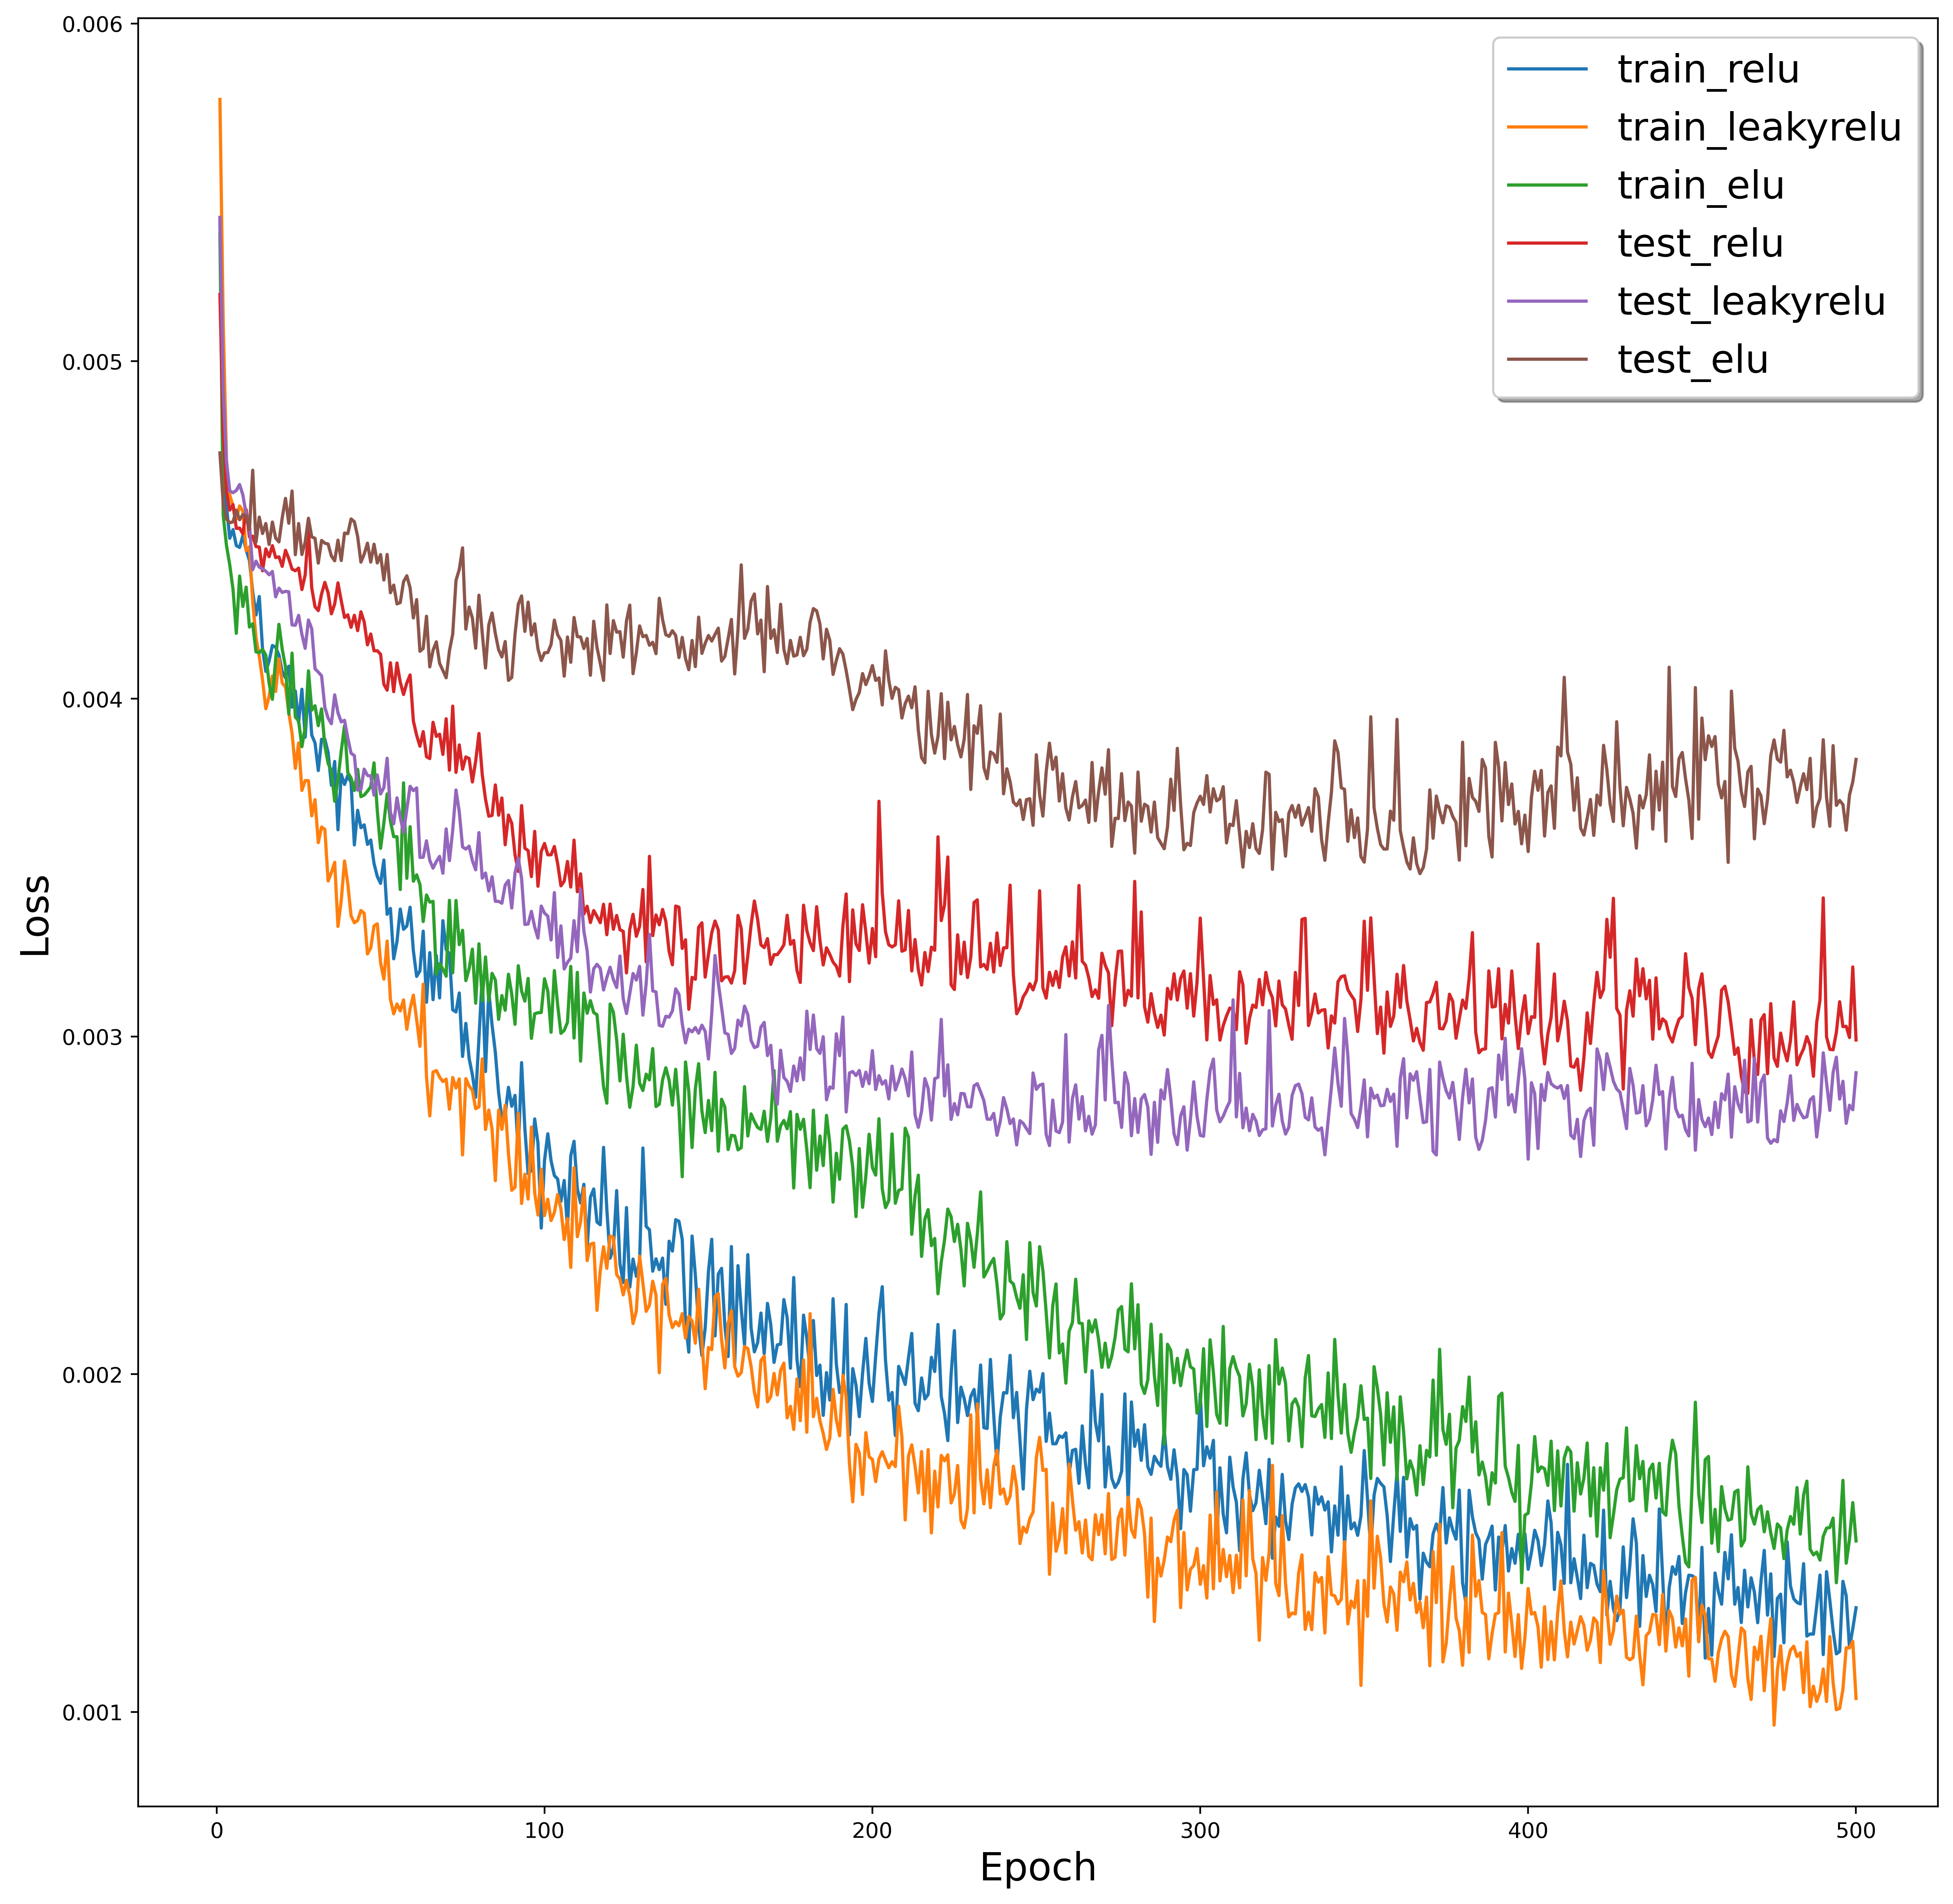
\includegraphics[width=0.45\textwidth]{results/eegnet_adam_128_0.001_0.5_loss.png}
		\caption{EEGNet with Adam, 128 batch size, \\ $1 \times 10^{-3}$ learning rate, and 50\% dropout.}
   	\end{figure}
	\begin{figure}[H]
	  \centering
		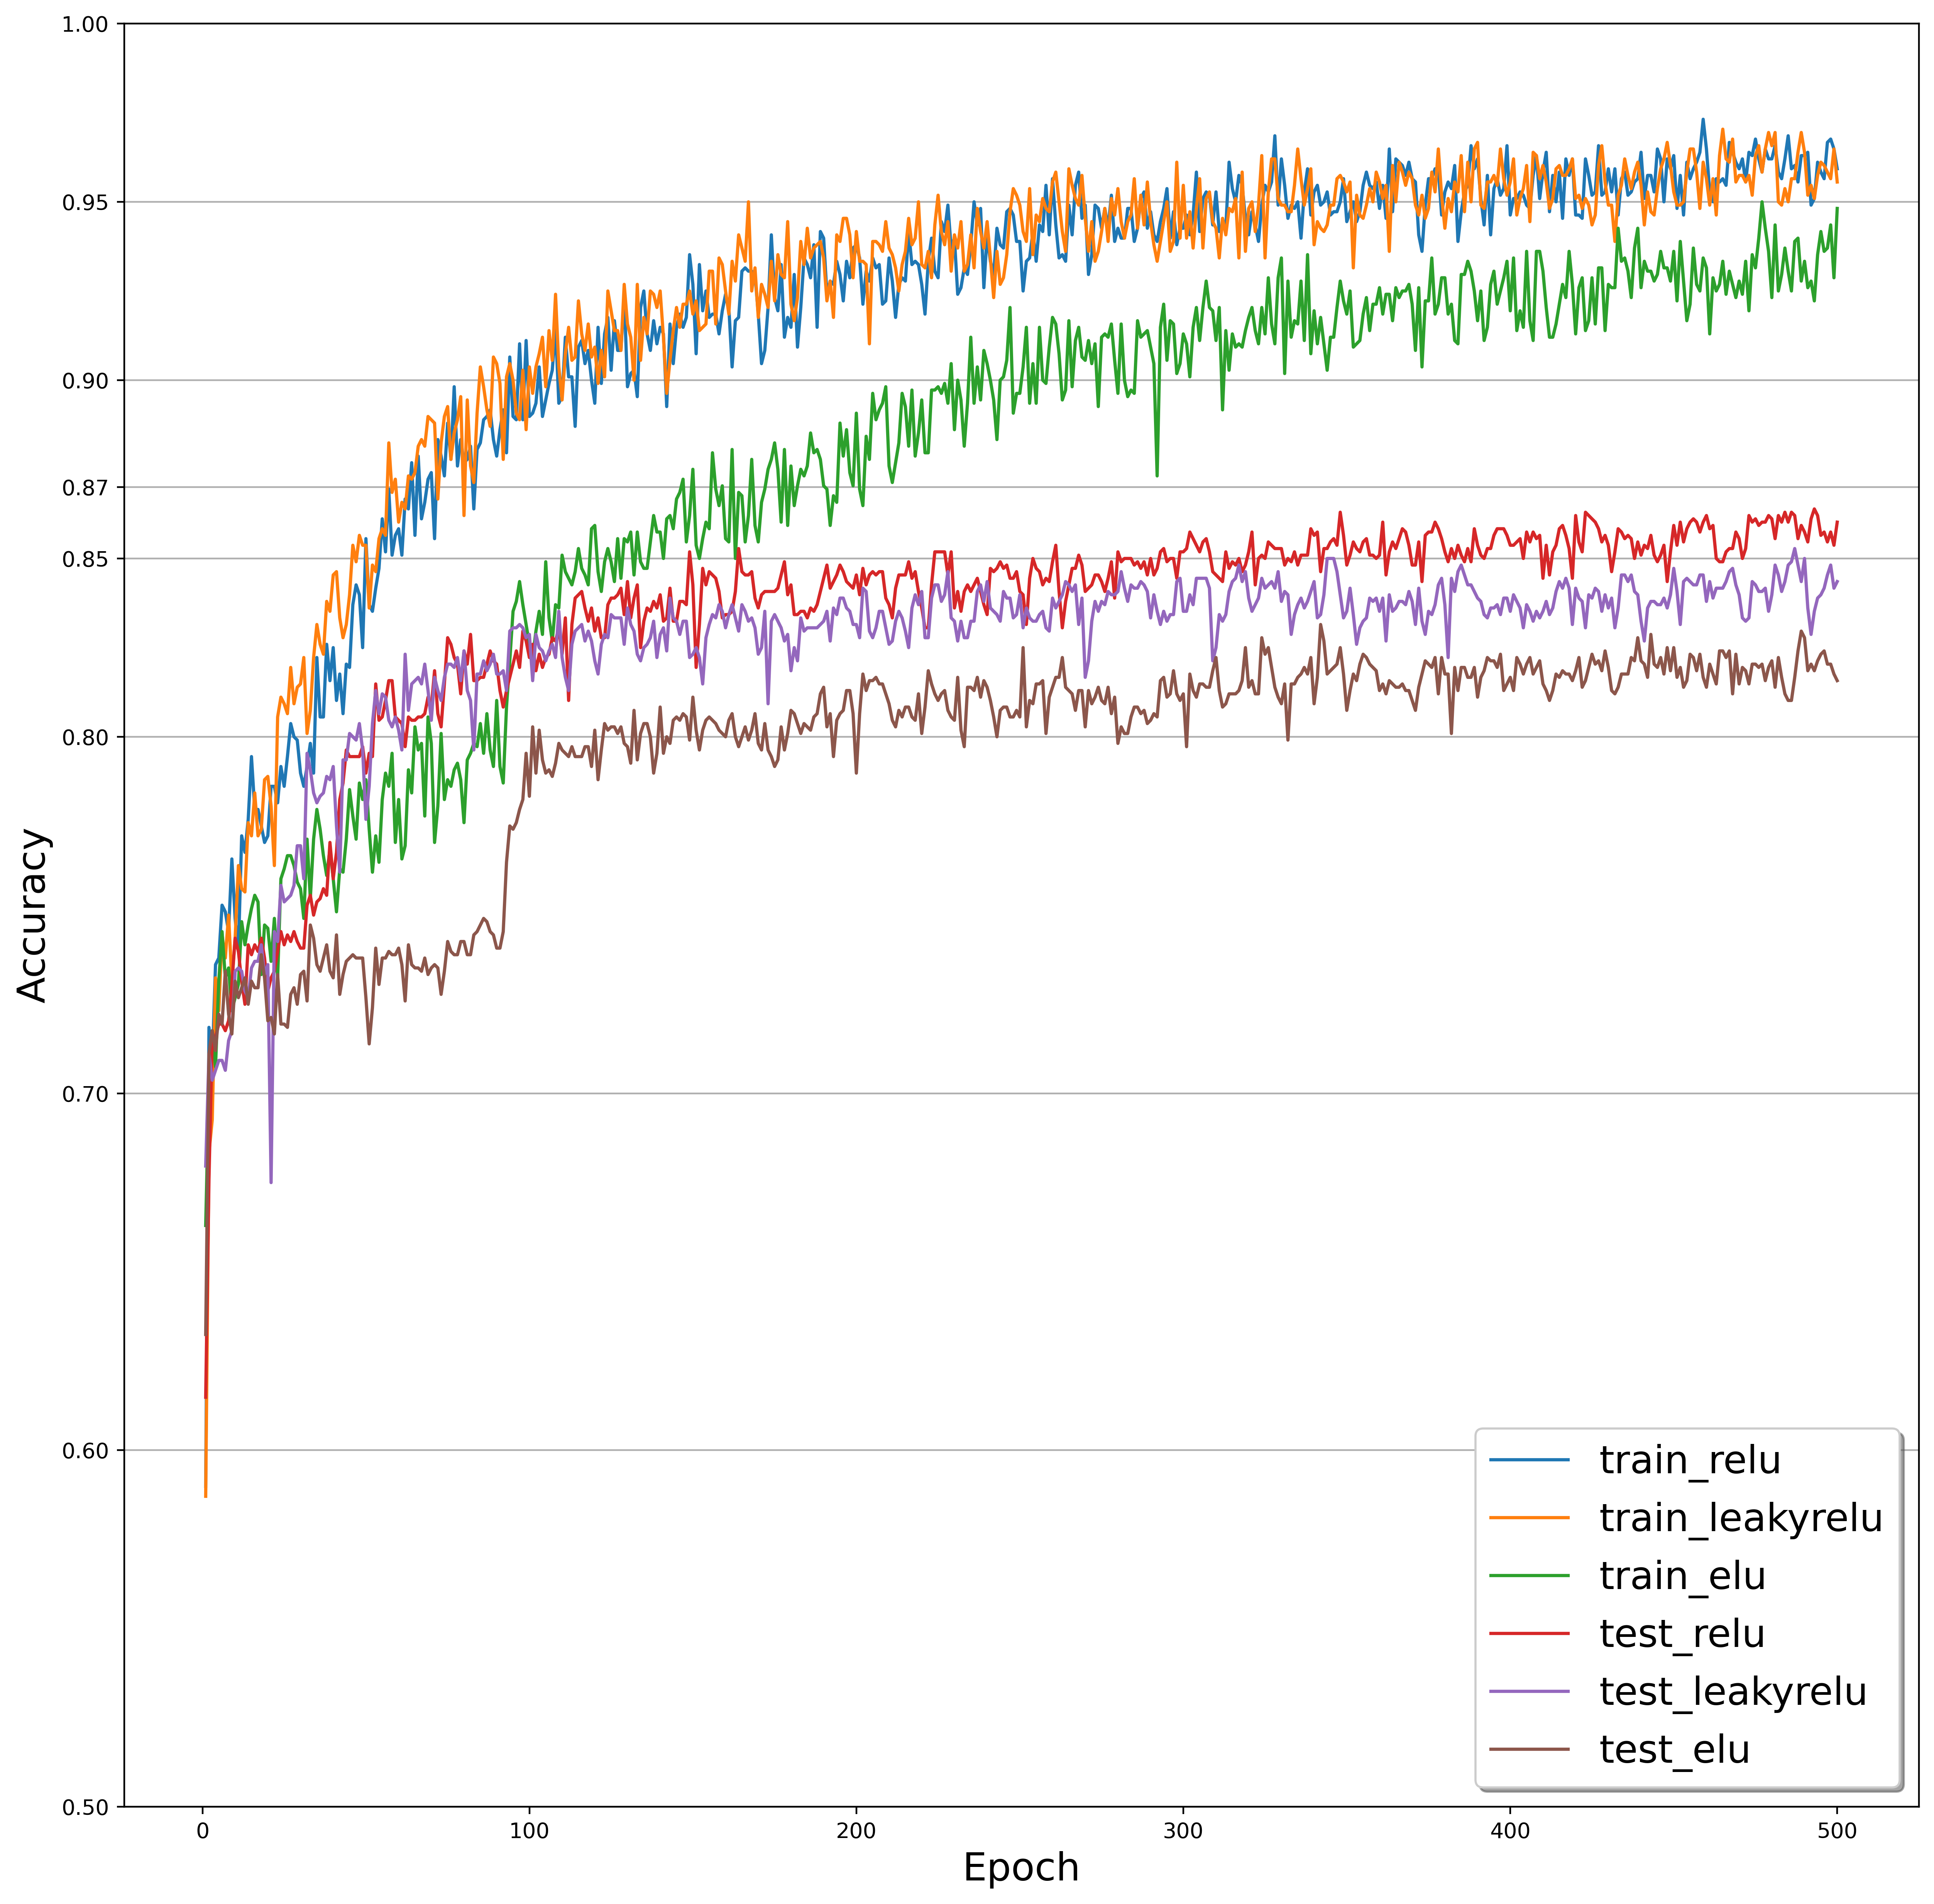
\includegraphics[width=0.45\textwidth]{results/eegnet_adam_128_0.01_0.5_acc.png}
		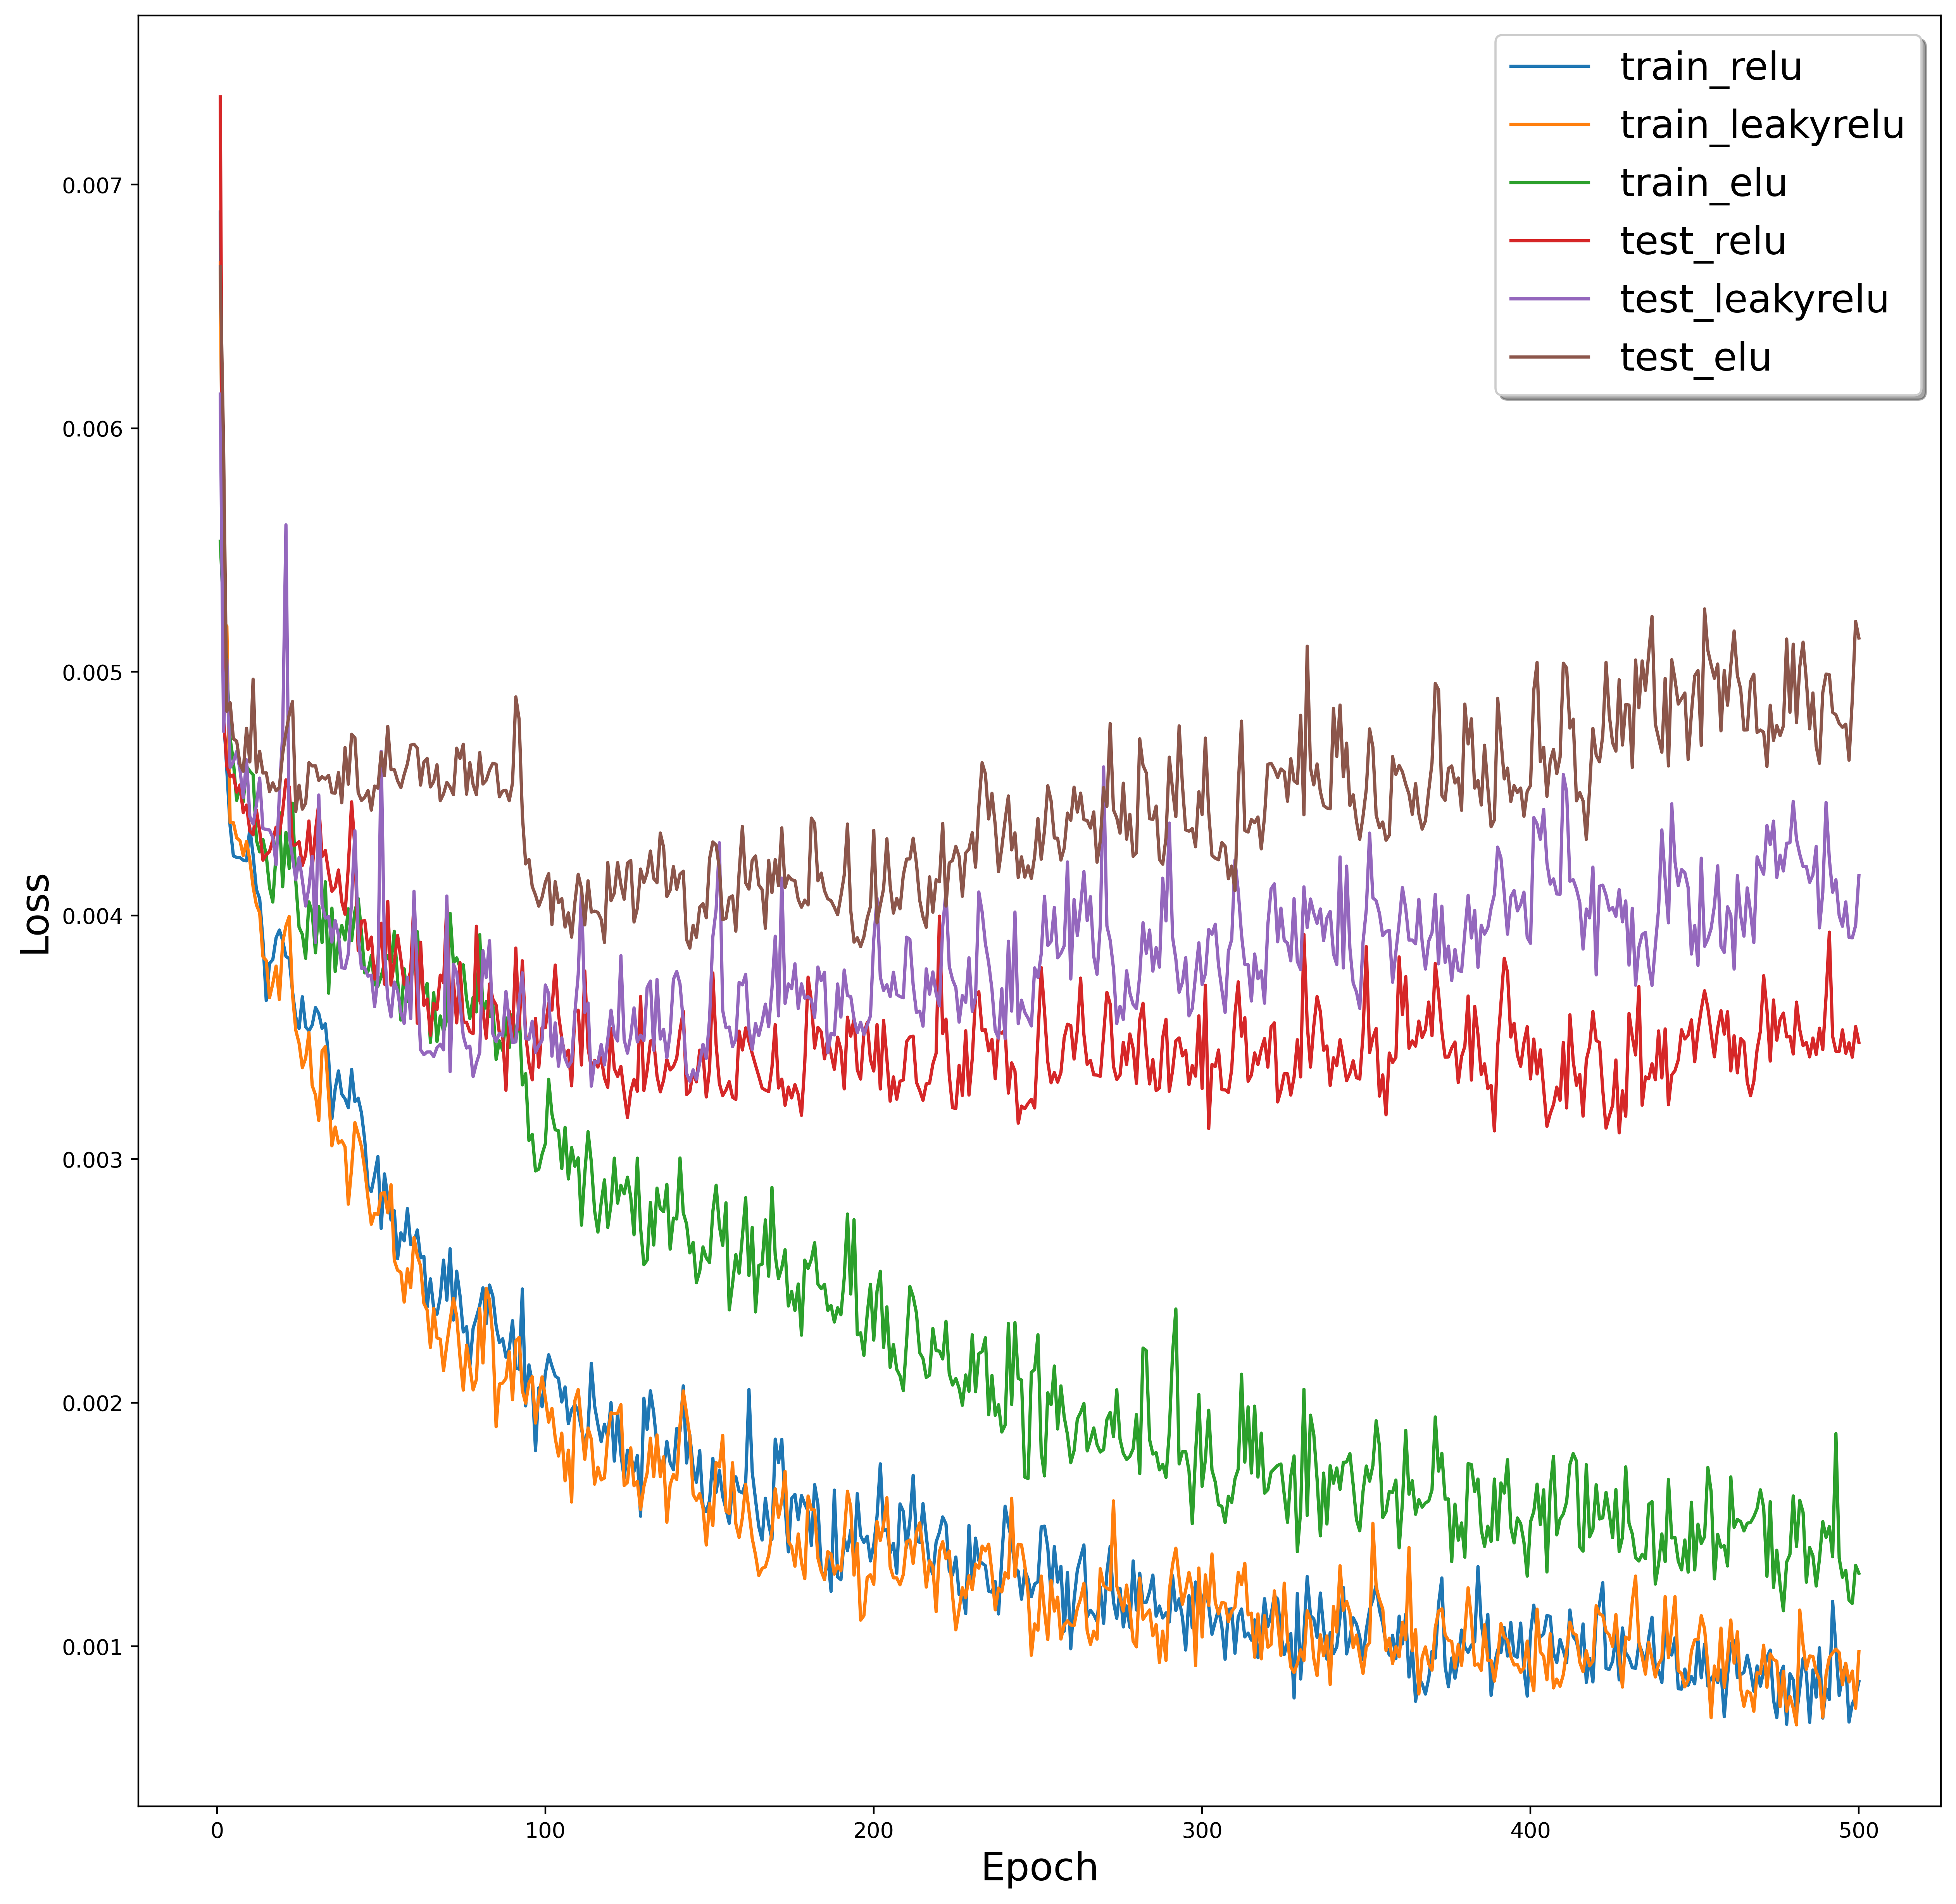
\includegraphics[width=0.45\textwidth]{results/eegnet_adam_128_0.01_0.5_loss.png}
		\caption{EEGNet with Adam, 128 batch size, \\ $1 \times 10^{-2}$ learning rate, and 50\% dropout.}
   	\end{figure}
	\begin{figure}[H]
		\centering
		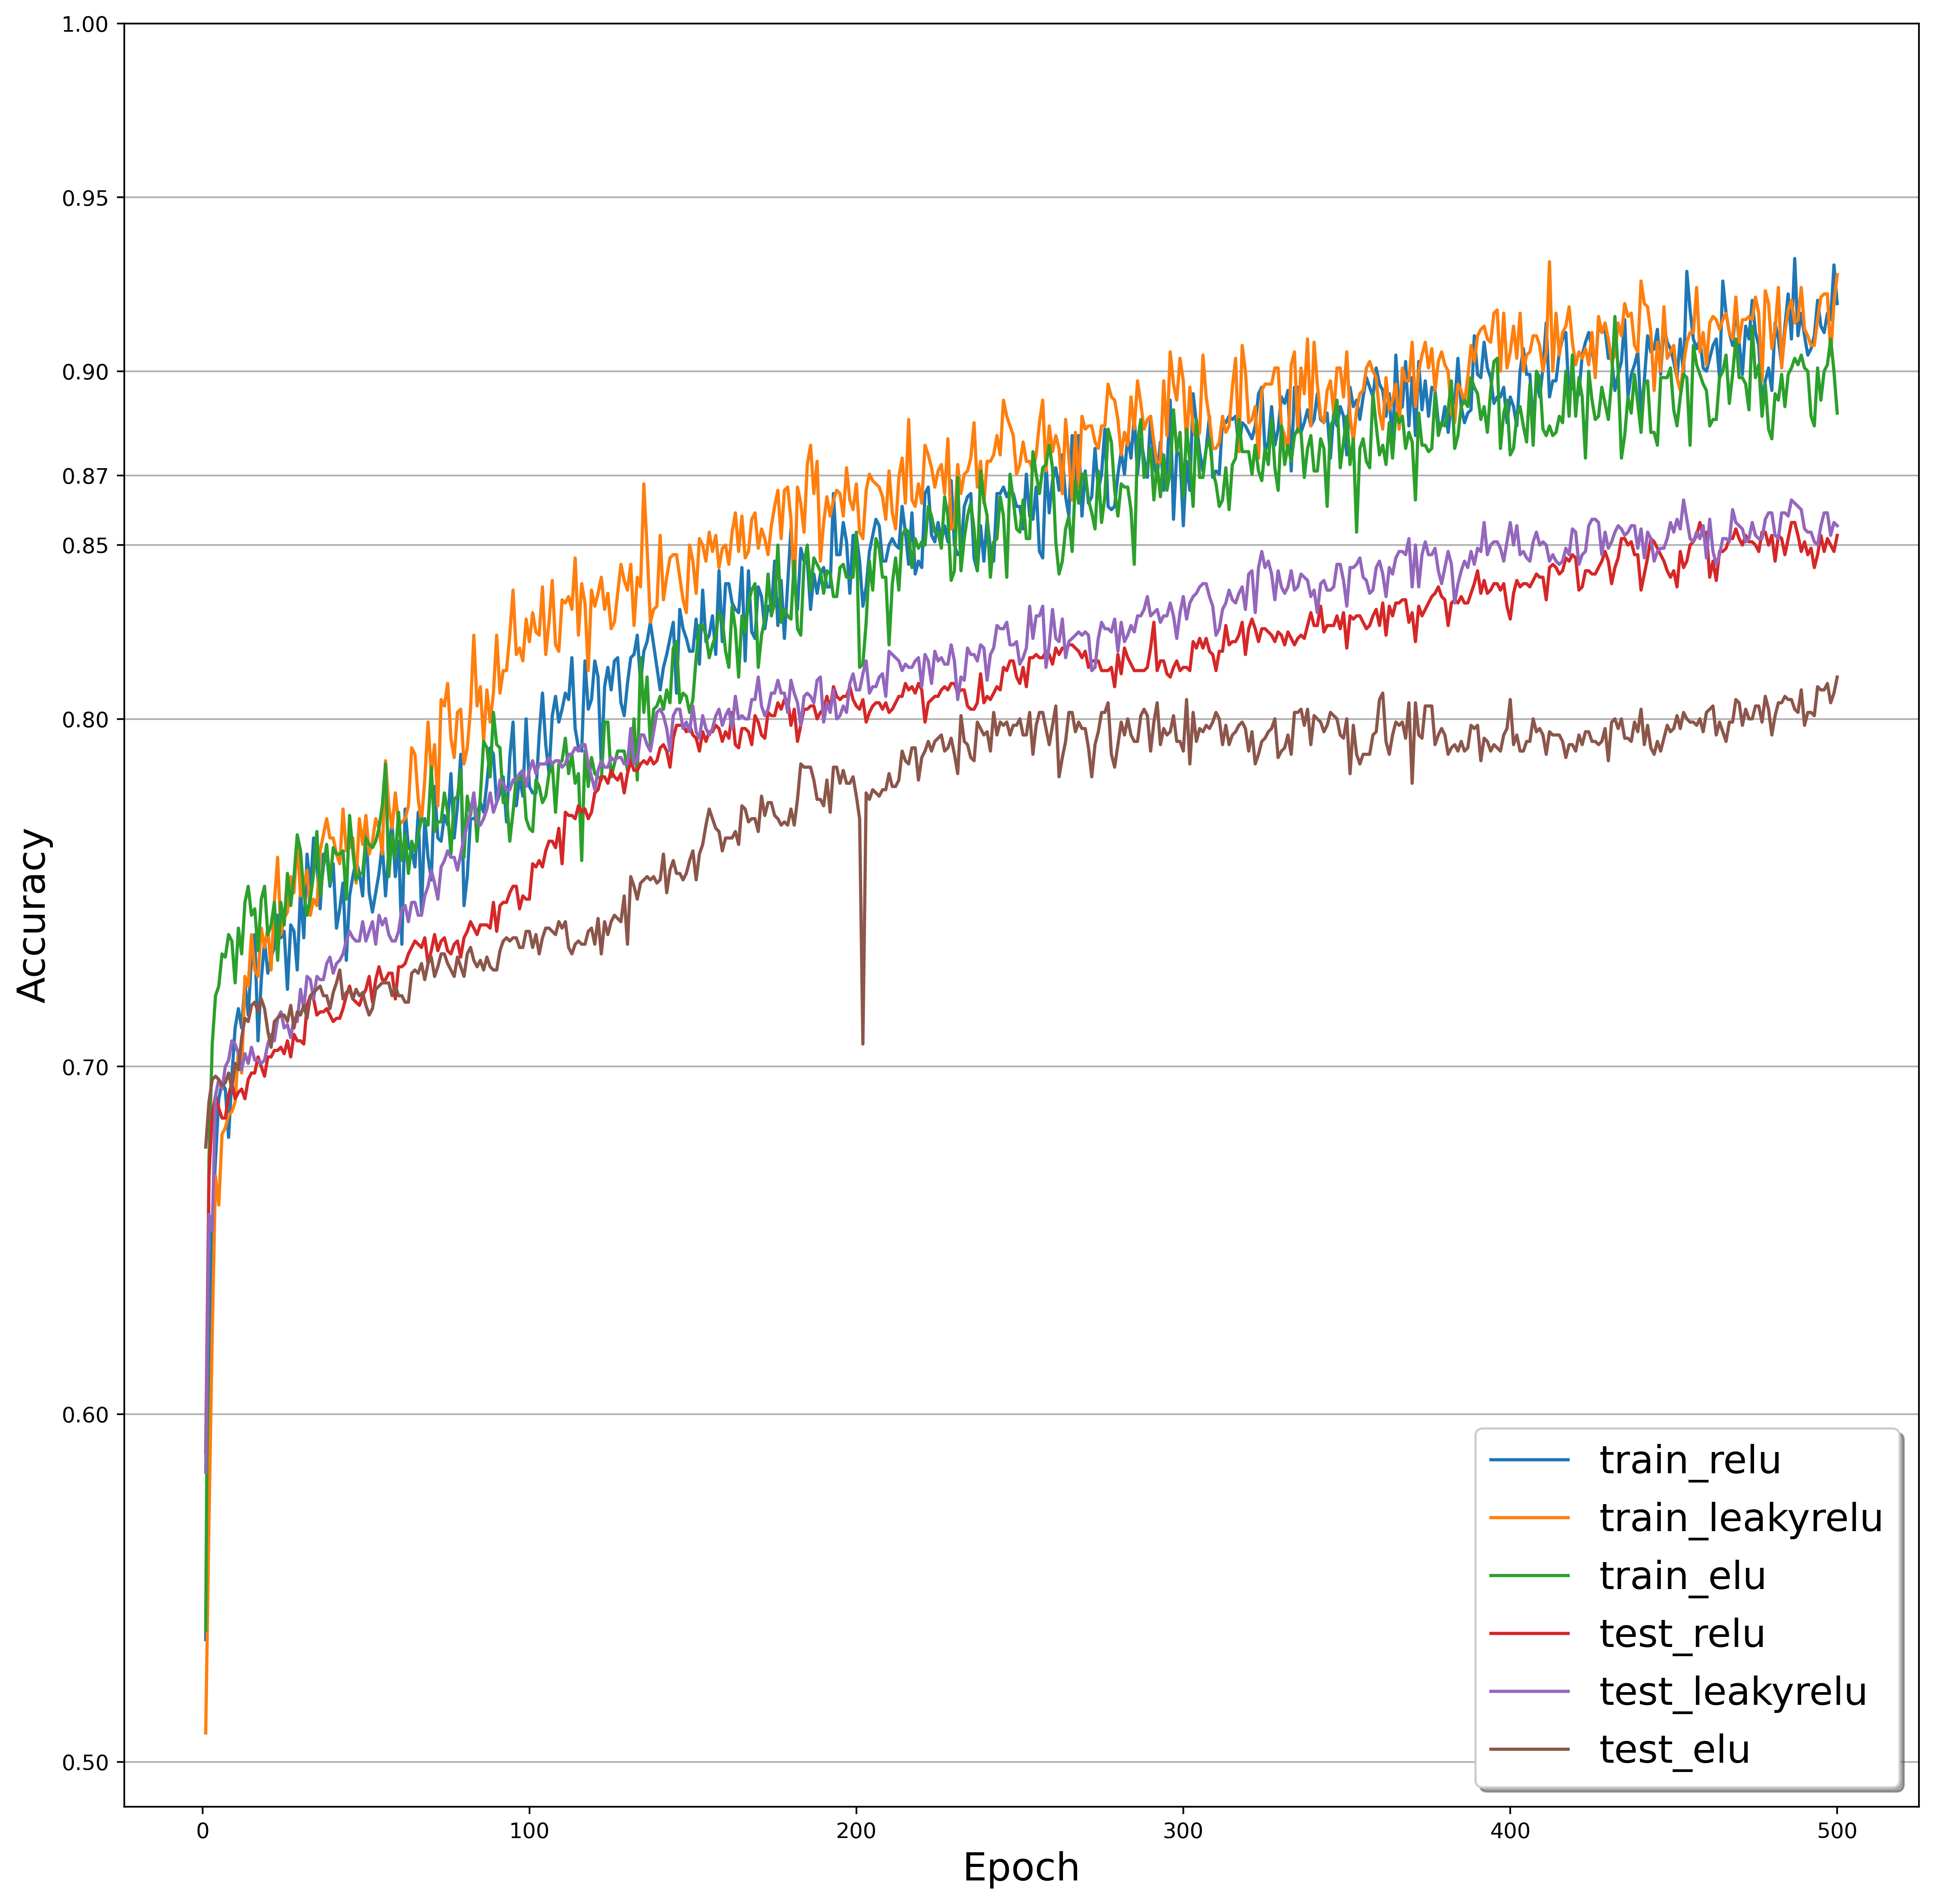
\includegraphics[width=0.45\textwidth]{results/eegnet_sgd_128_0.005_0.5_acc.png}
		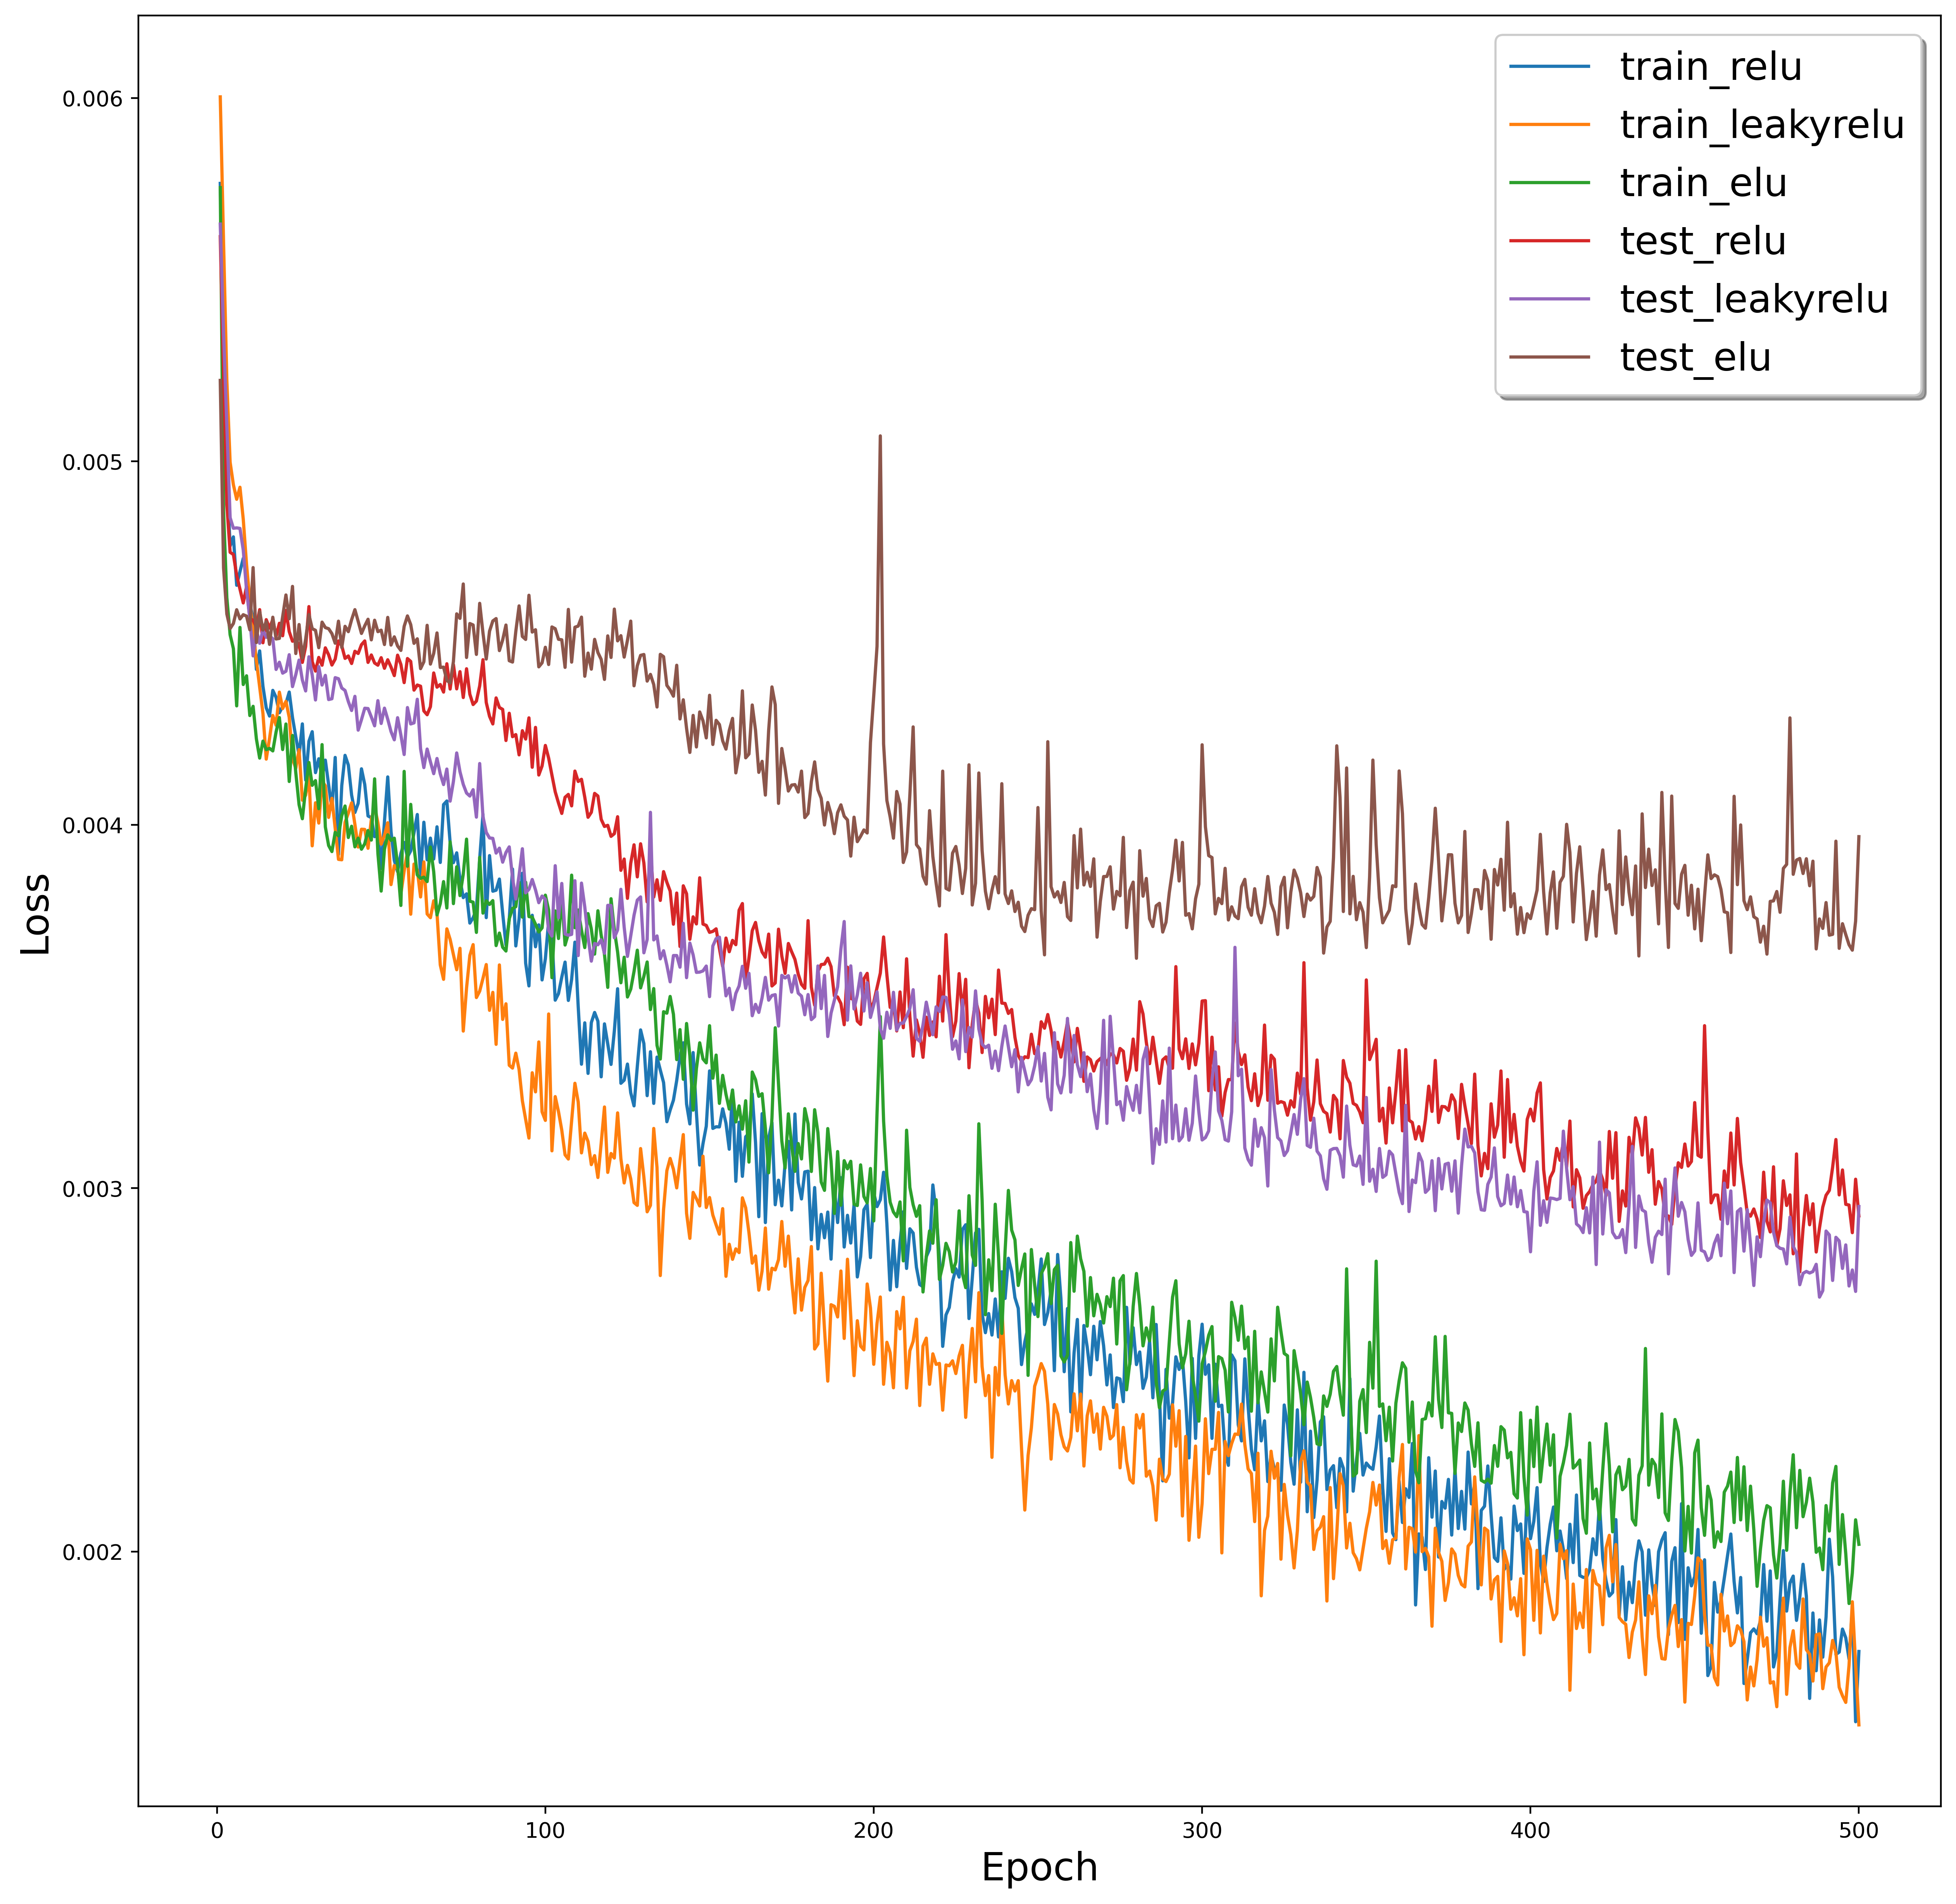
\includegraphics[width=0.45\textwidth]{results/eegnet_sgd_128_0.005_0.5_loss.png}
		\caption{EEGNet with SGD, 128 batch size, \\ $5 \times 10^{-3}$ learning rate, and 50\% dropout.}
   	\end{figure}
	\begin{figure}[H]
	  \centering
		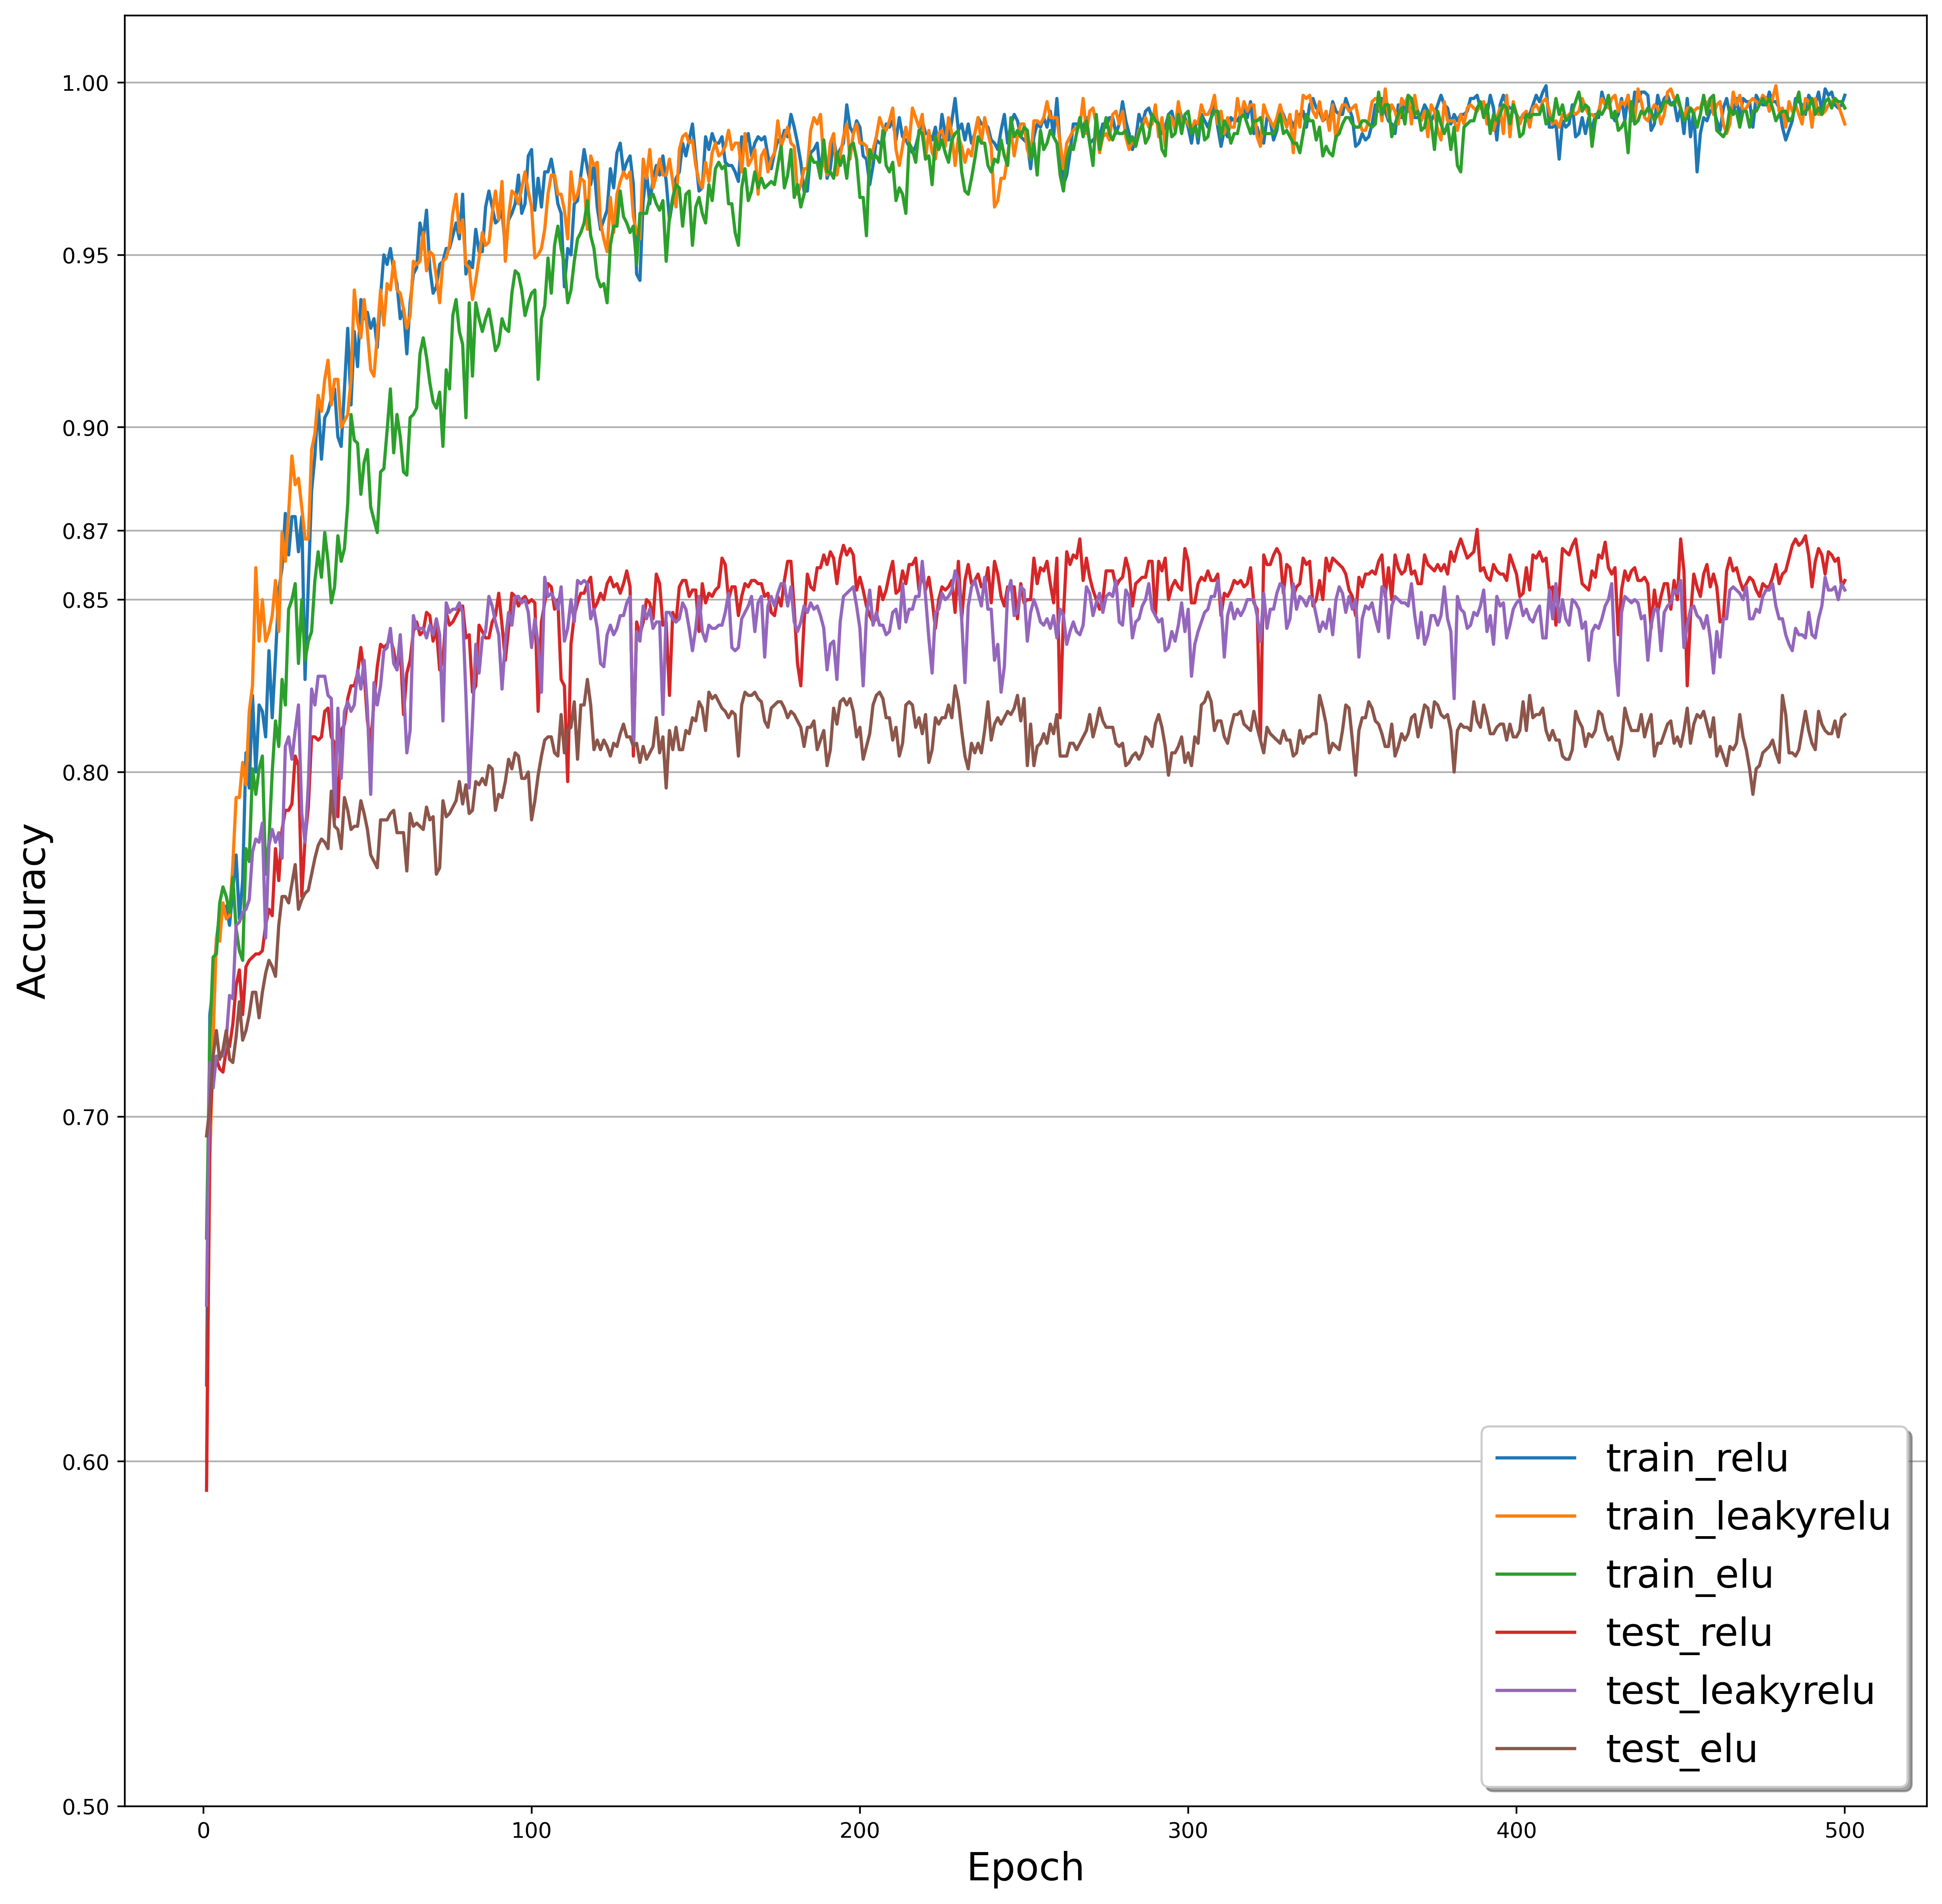
\includegraphics[width=0.45\textwidth]{results/eegnet_adam_128_0.005_0.25_acc.png}
		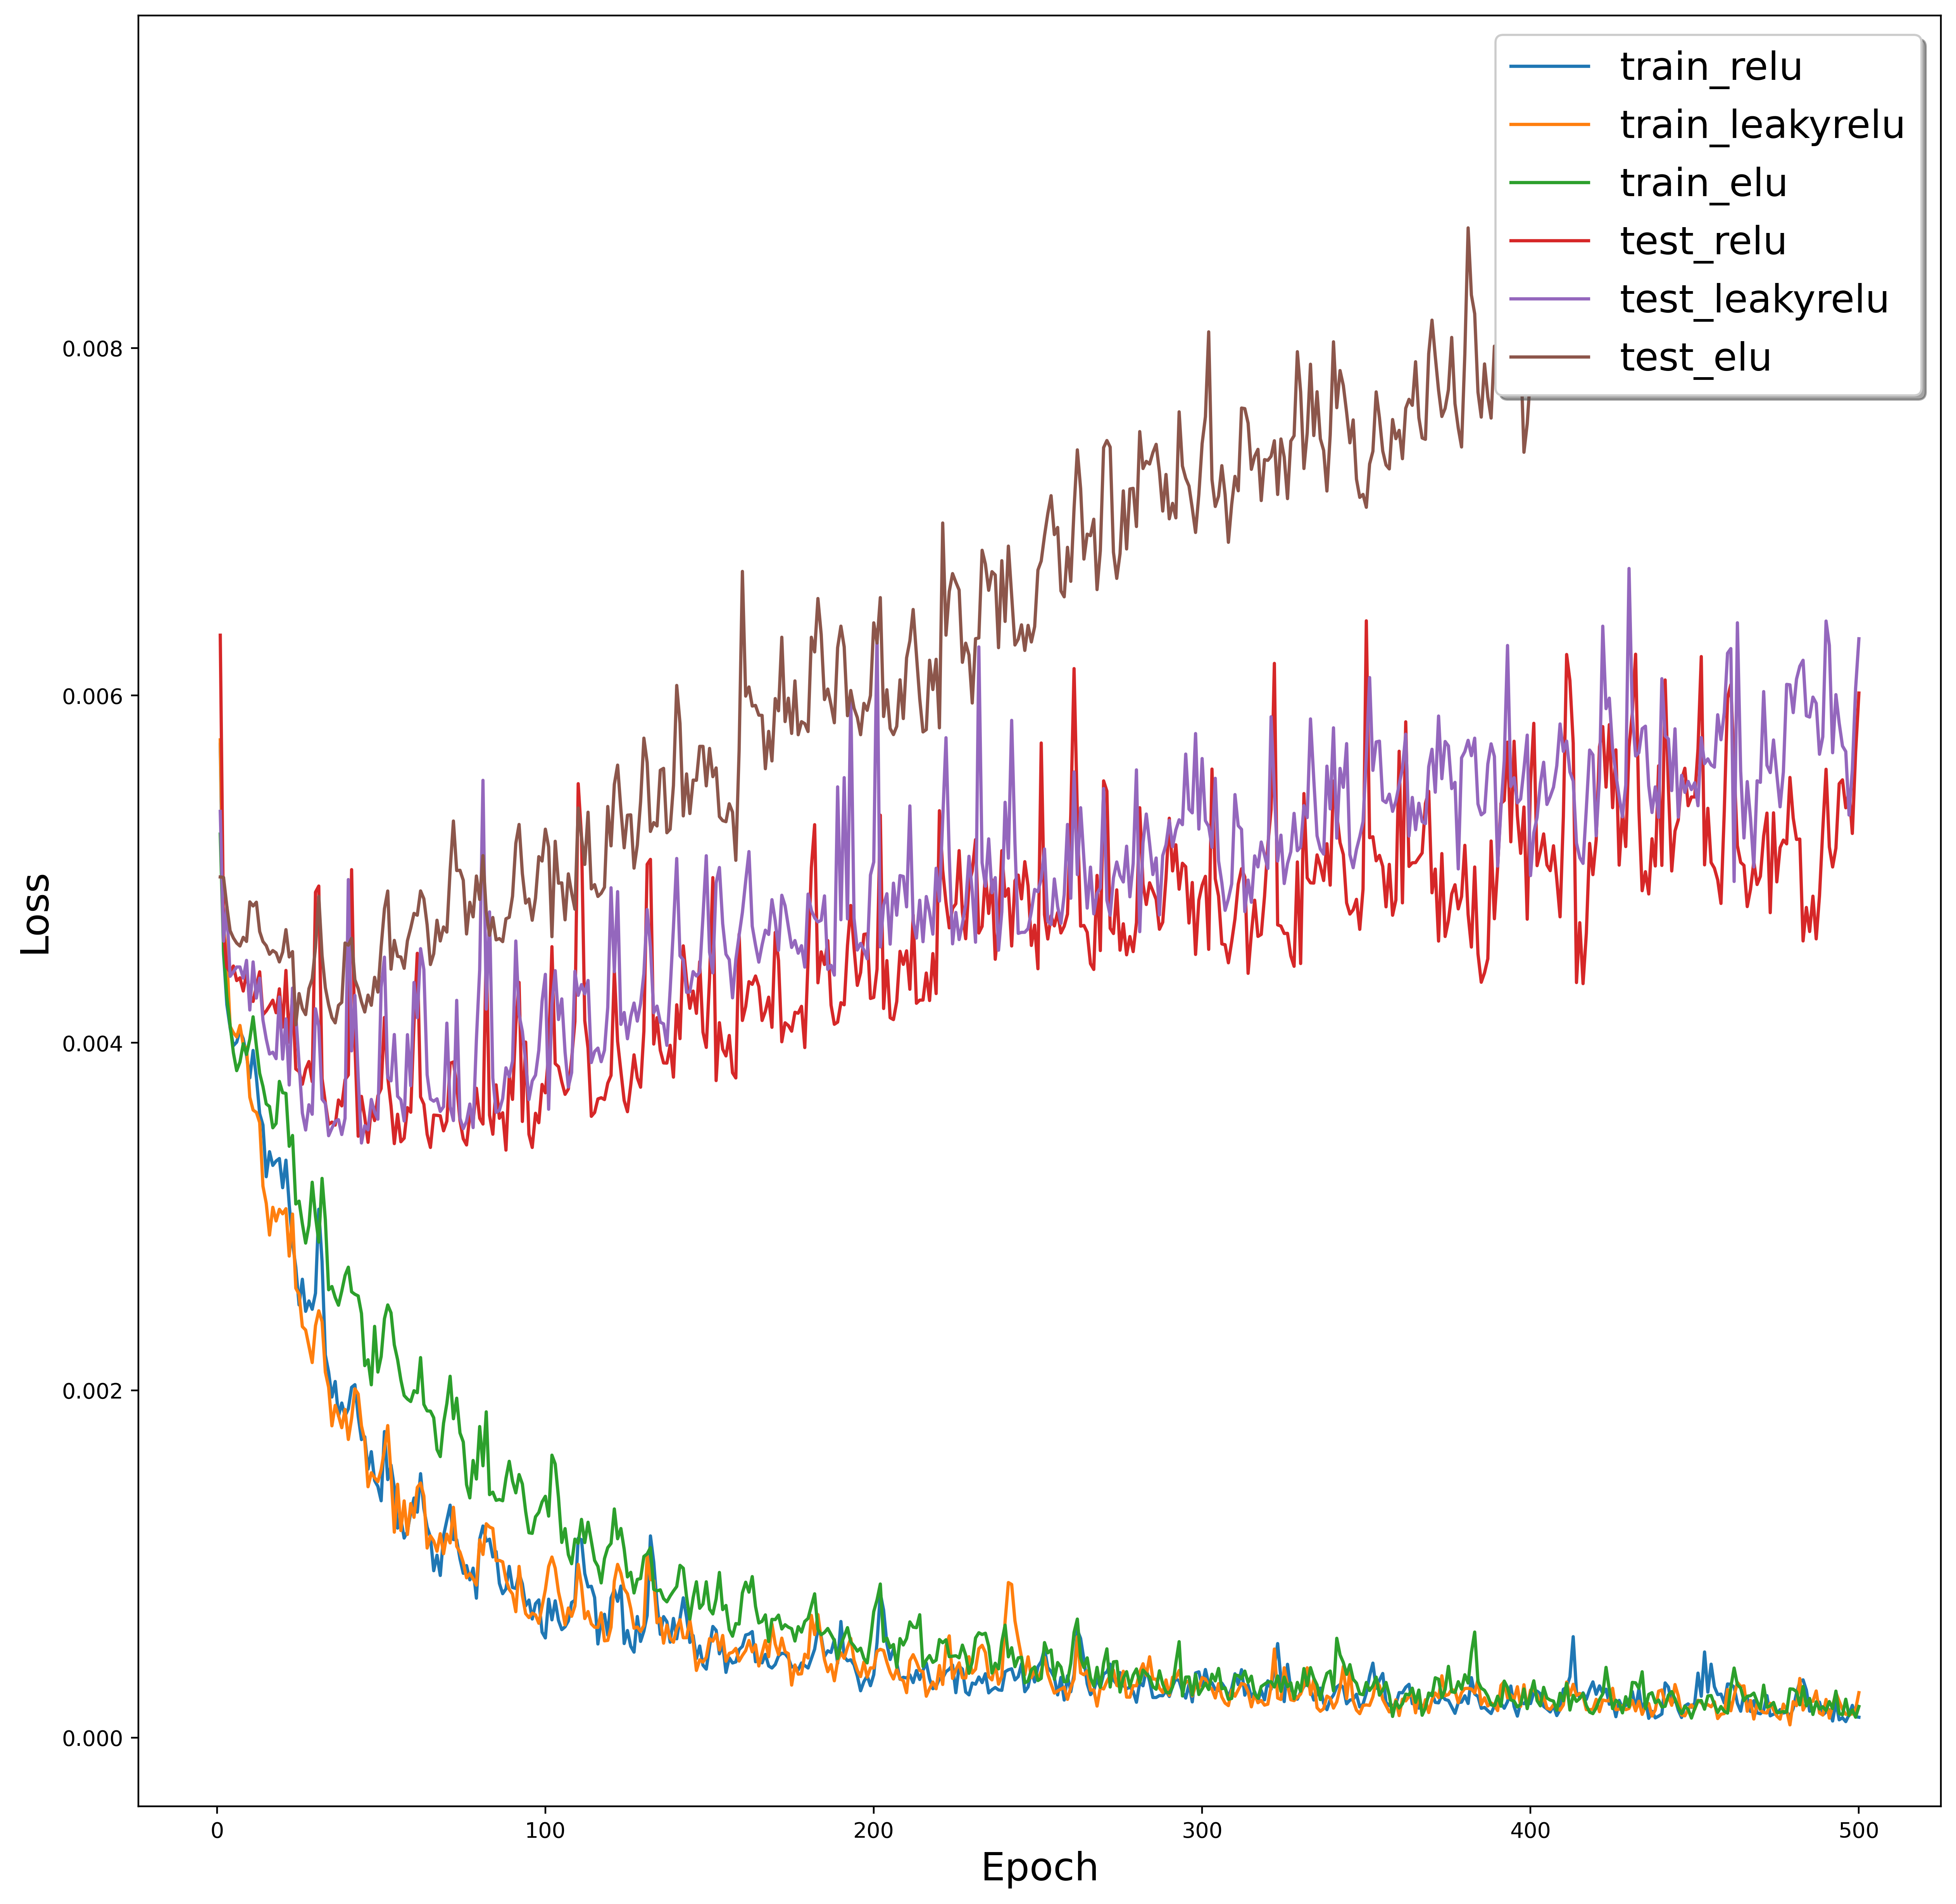
\includegraphics[width=0.45\textwidth]{results/eegnet_adam_128_0.005_0.25_loss.png}
		\caption{EEGNet with Adam, 128 batch size, \\ $5 \times 10^{-3}$ learning rate, and 25\% dropout.}
   	\end{figure}
	\begin{figure}[H]
		\centering
		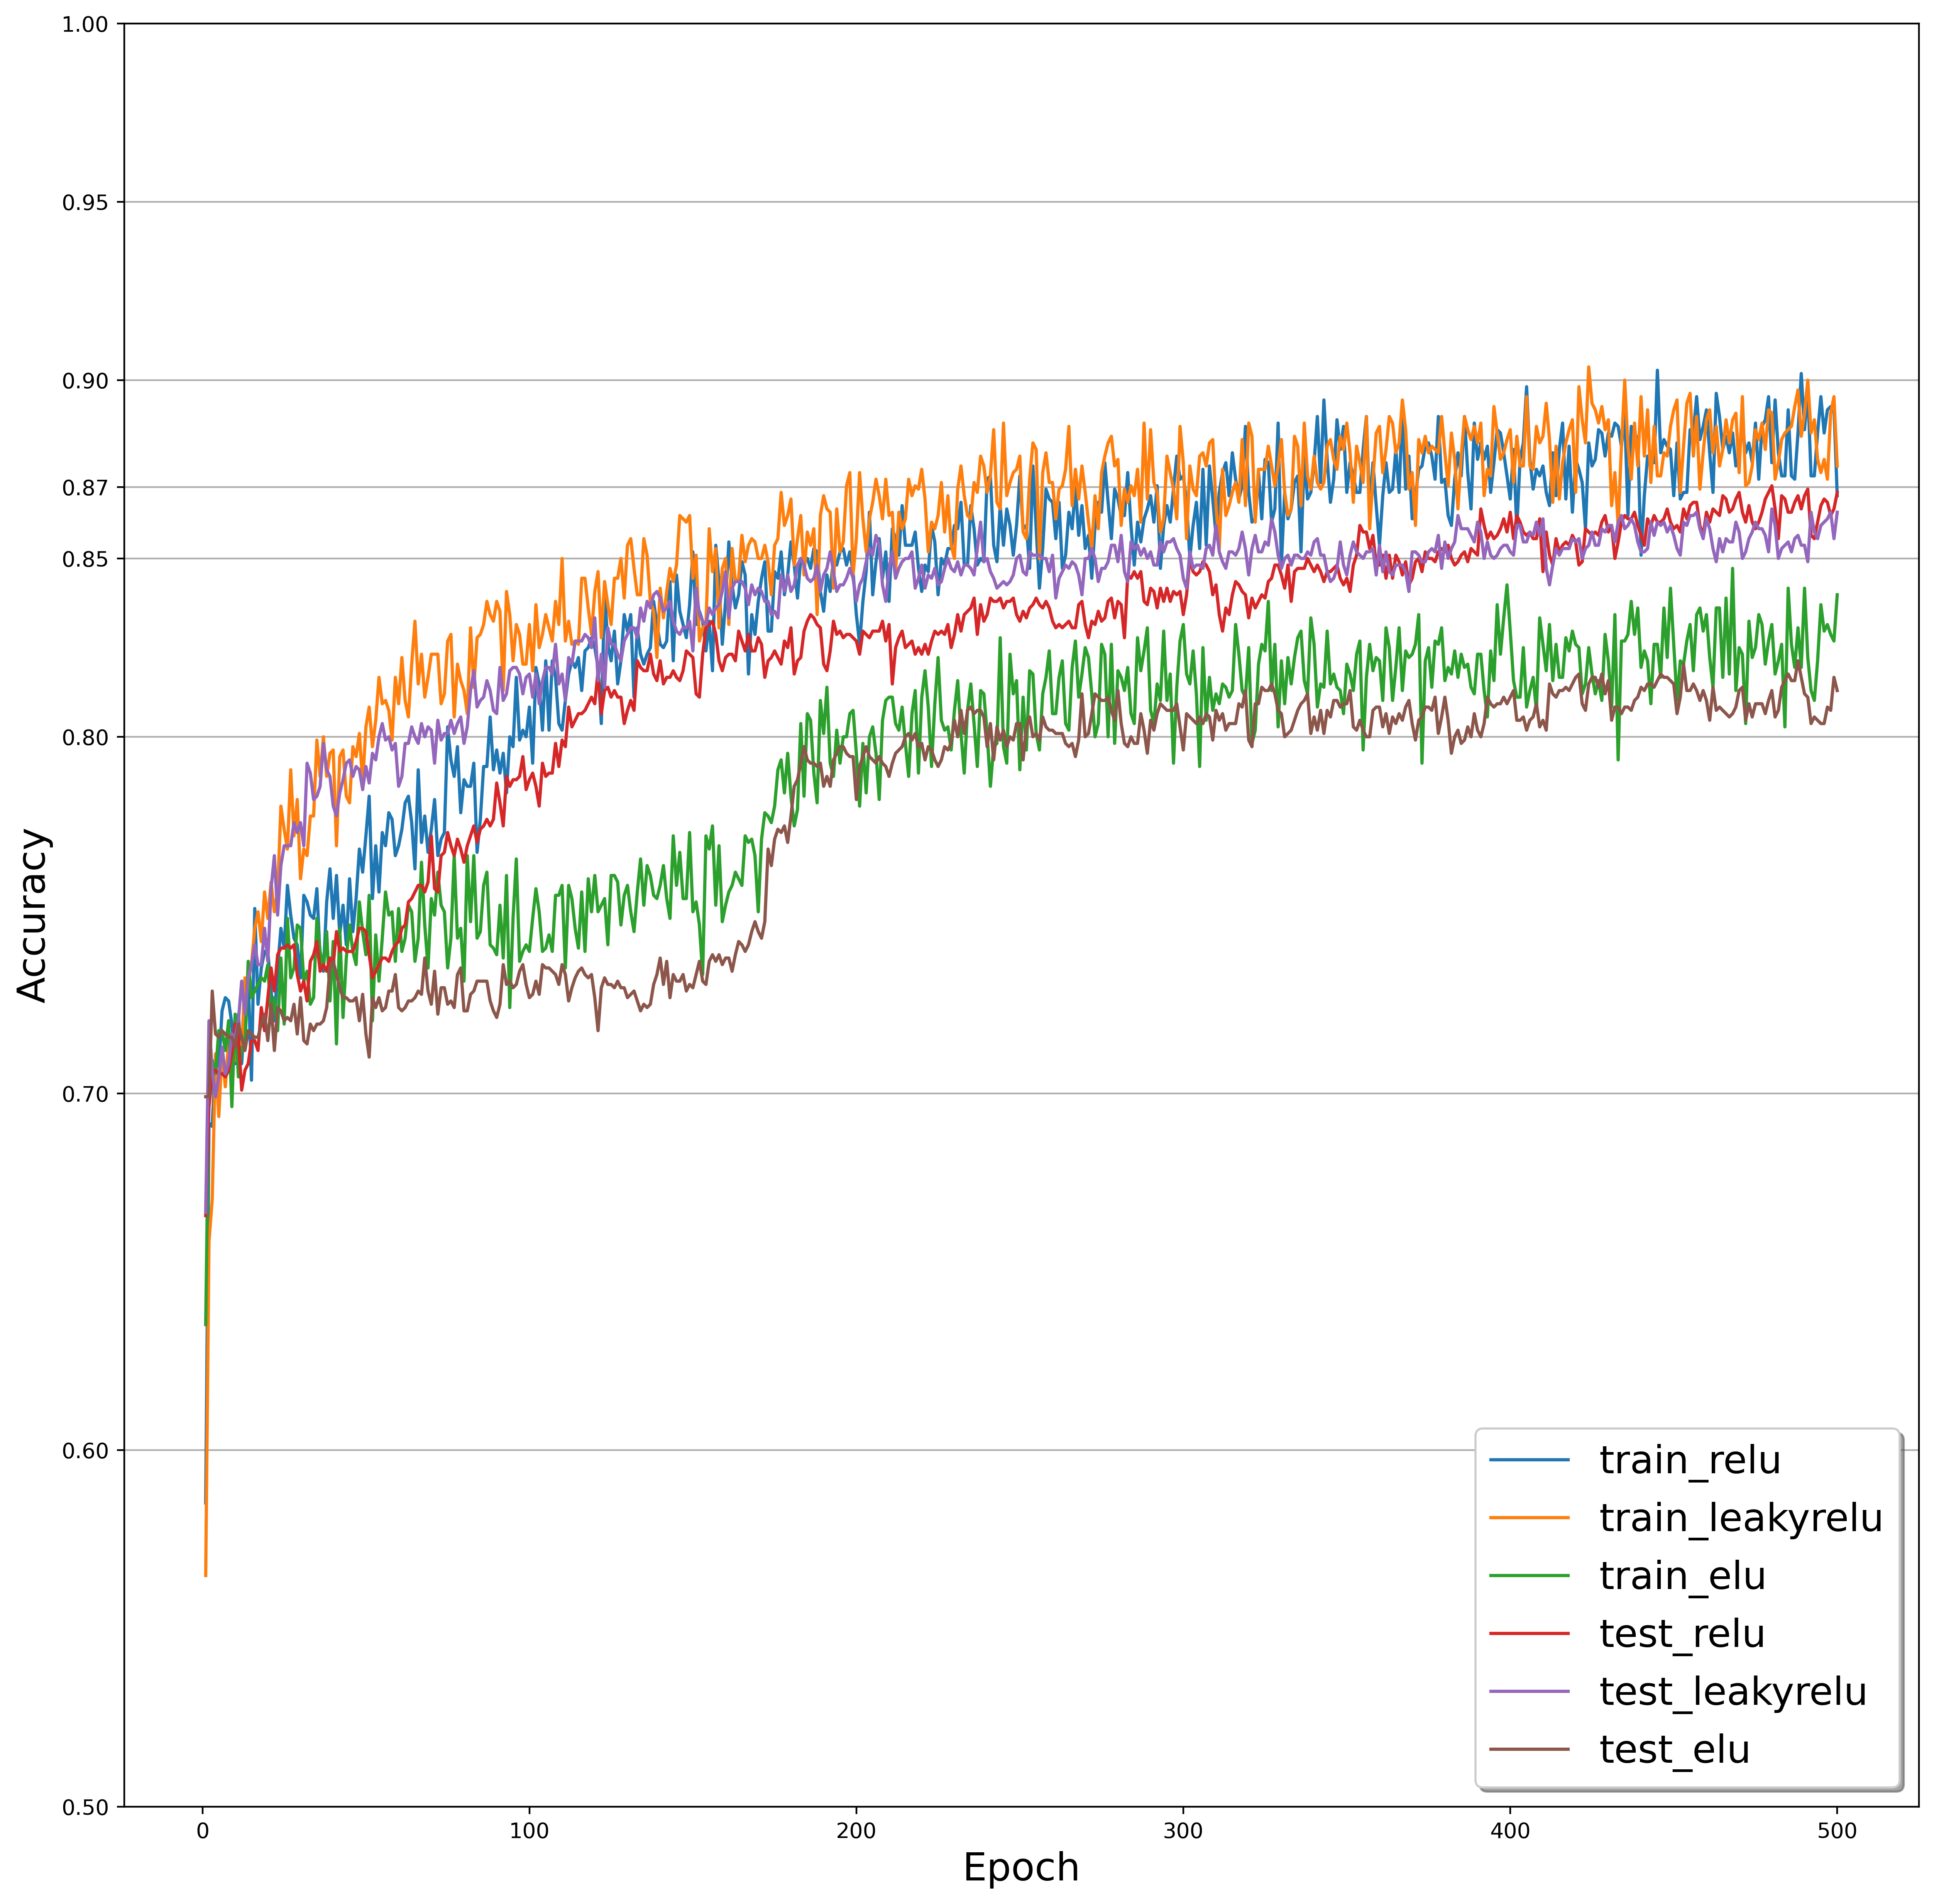
\includegraphics[width=0.45\textwidth]{results/eegnet_adam_128_0.005_0.75_acc.png}
		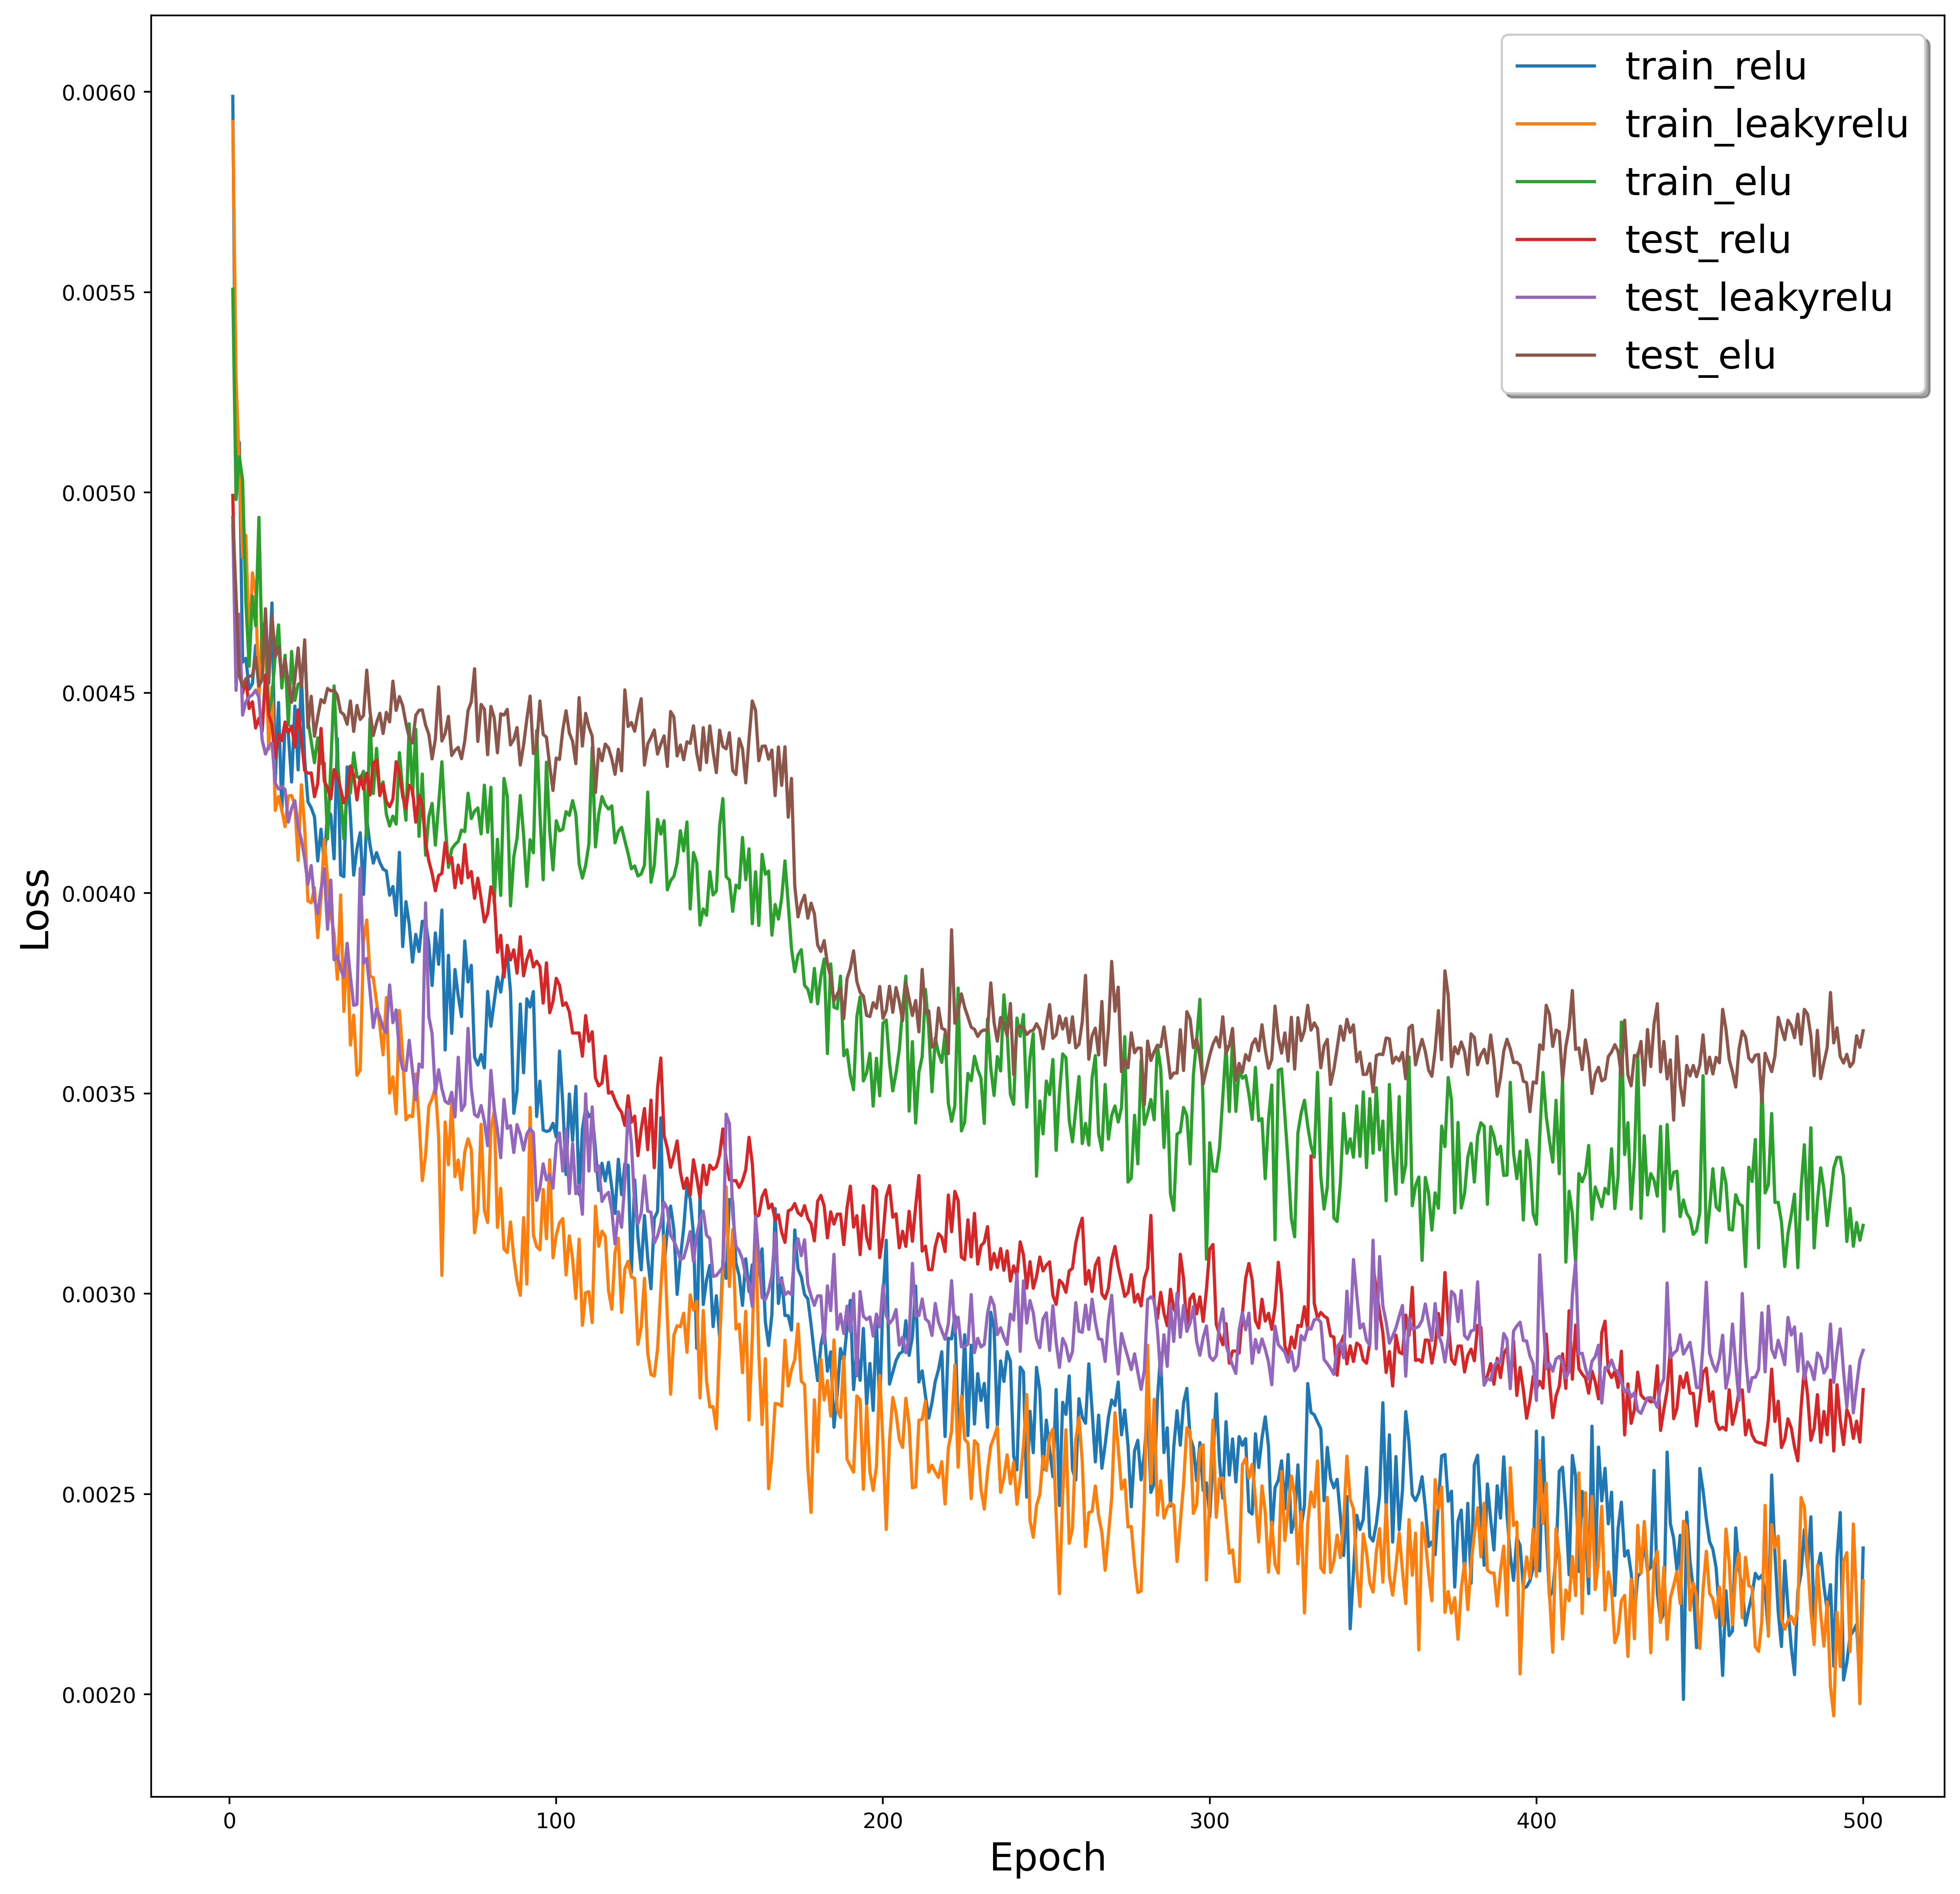
\includegraphics[width=0.45\textwidth]{results/eegnet_adam_128_0.005_0.75_loss.png}
		\caption{EEGNet with Adam, 128 batch size, \\ $5 \times 10^{-3}$ learning rate, and 75\% dropout.}
   	\end{figure}

\subsection{DeepConvNet}\label{results-deepconvnet}
	\begin{figure}[H]
		\centering
		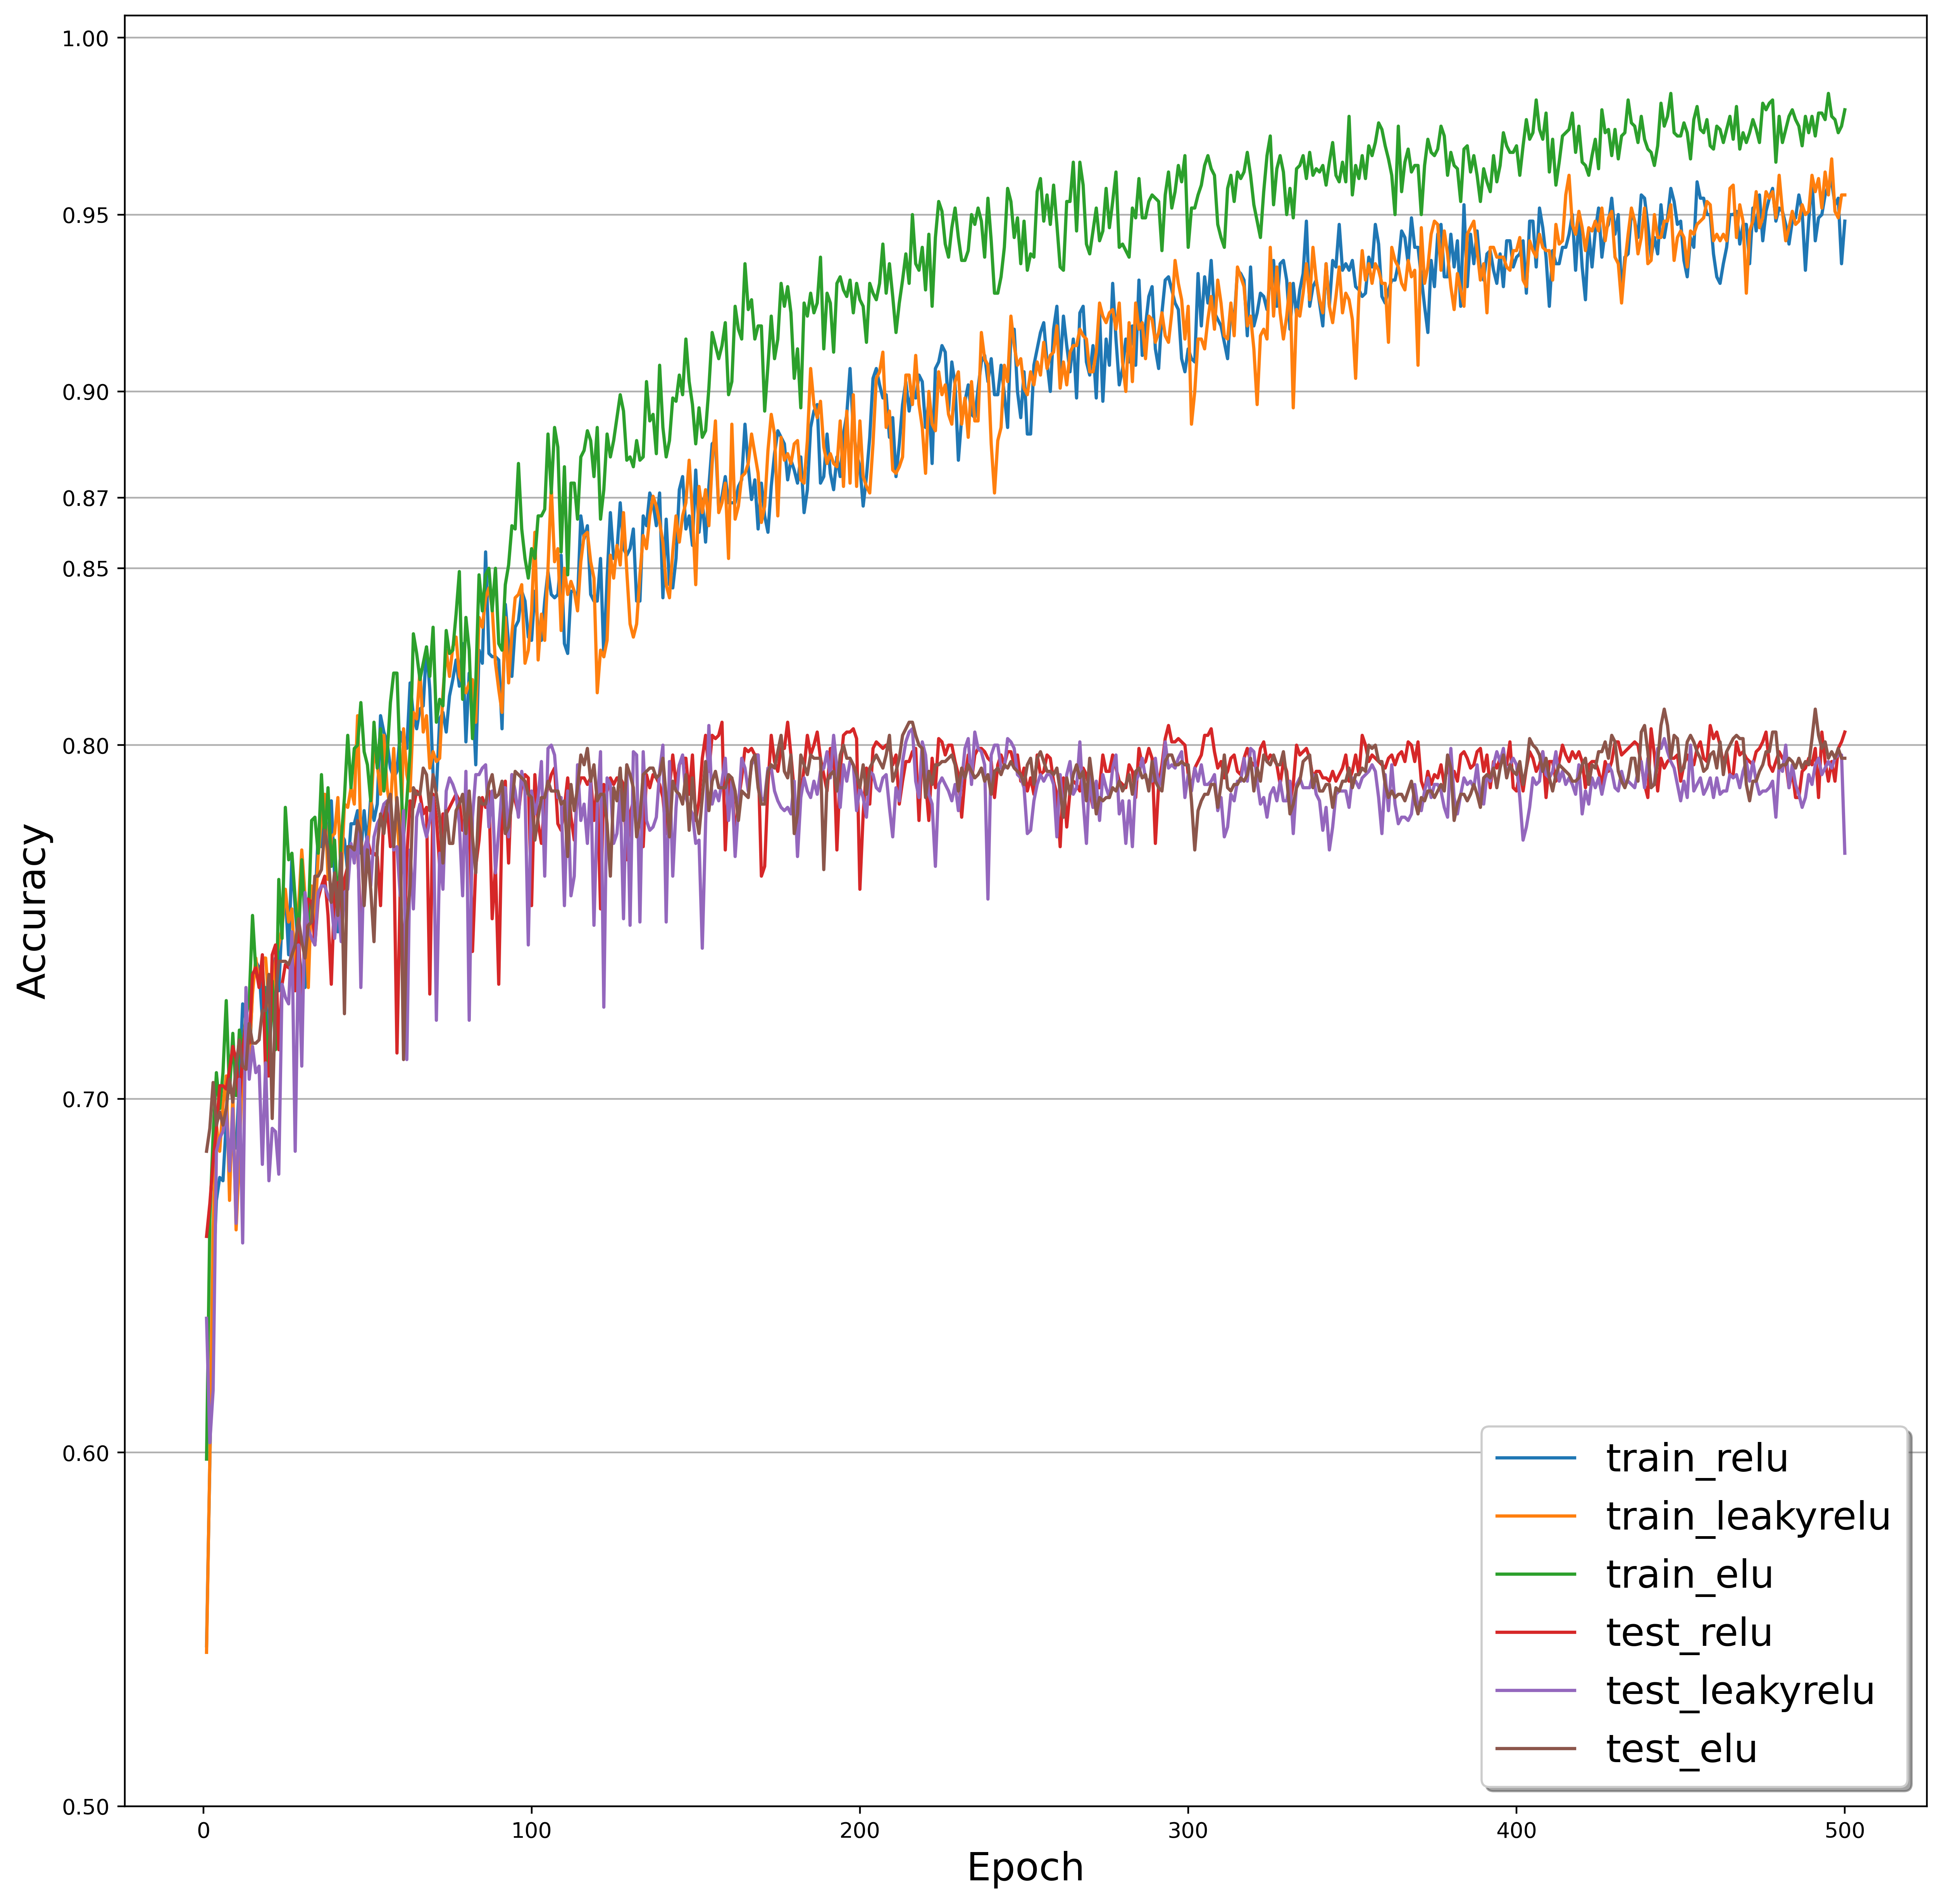
\includegraphics[width=0.45\textwidth]{results/deepconvnet_adam_32_0.0005_0.5_acc.png}
		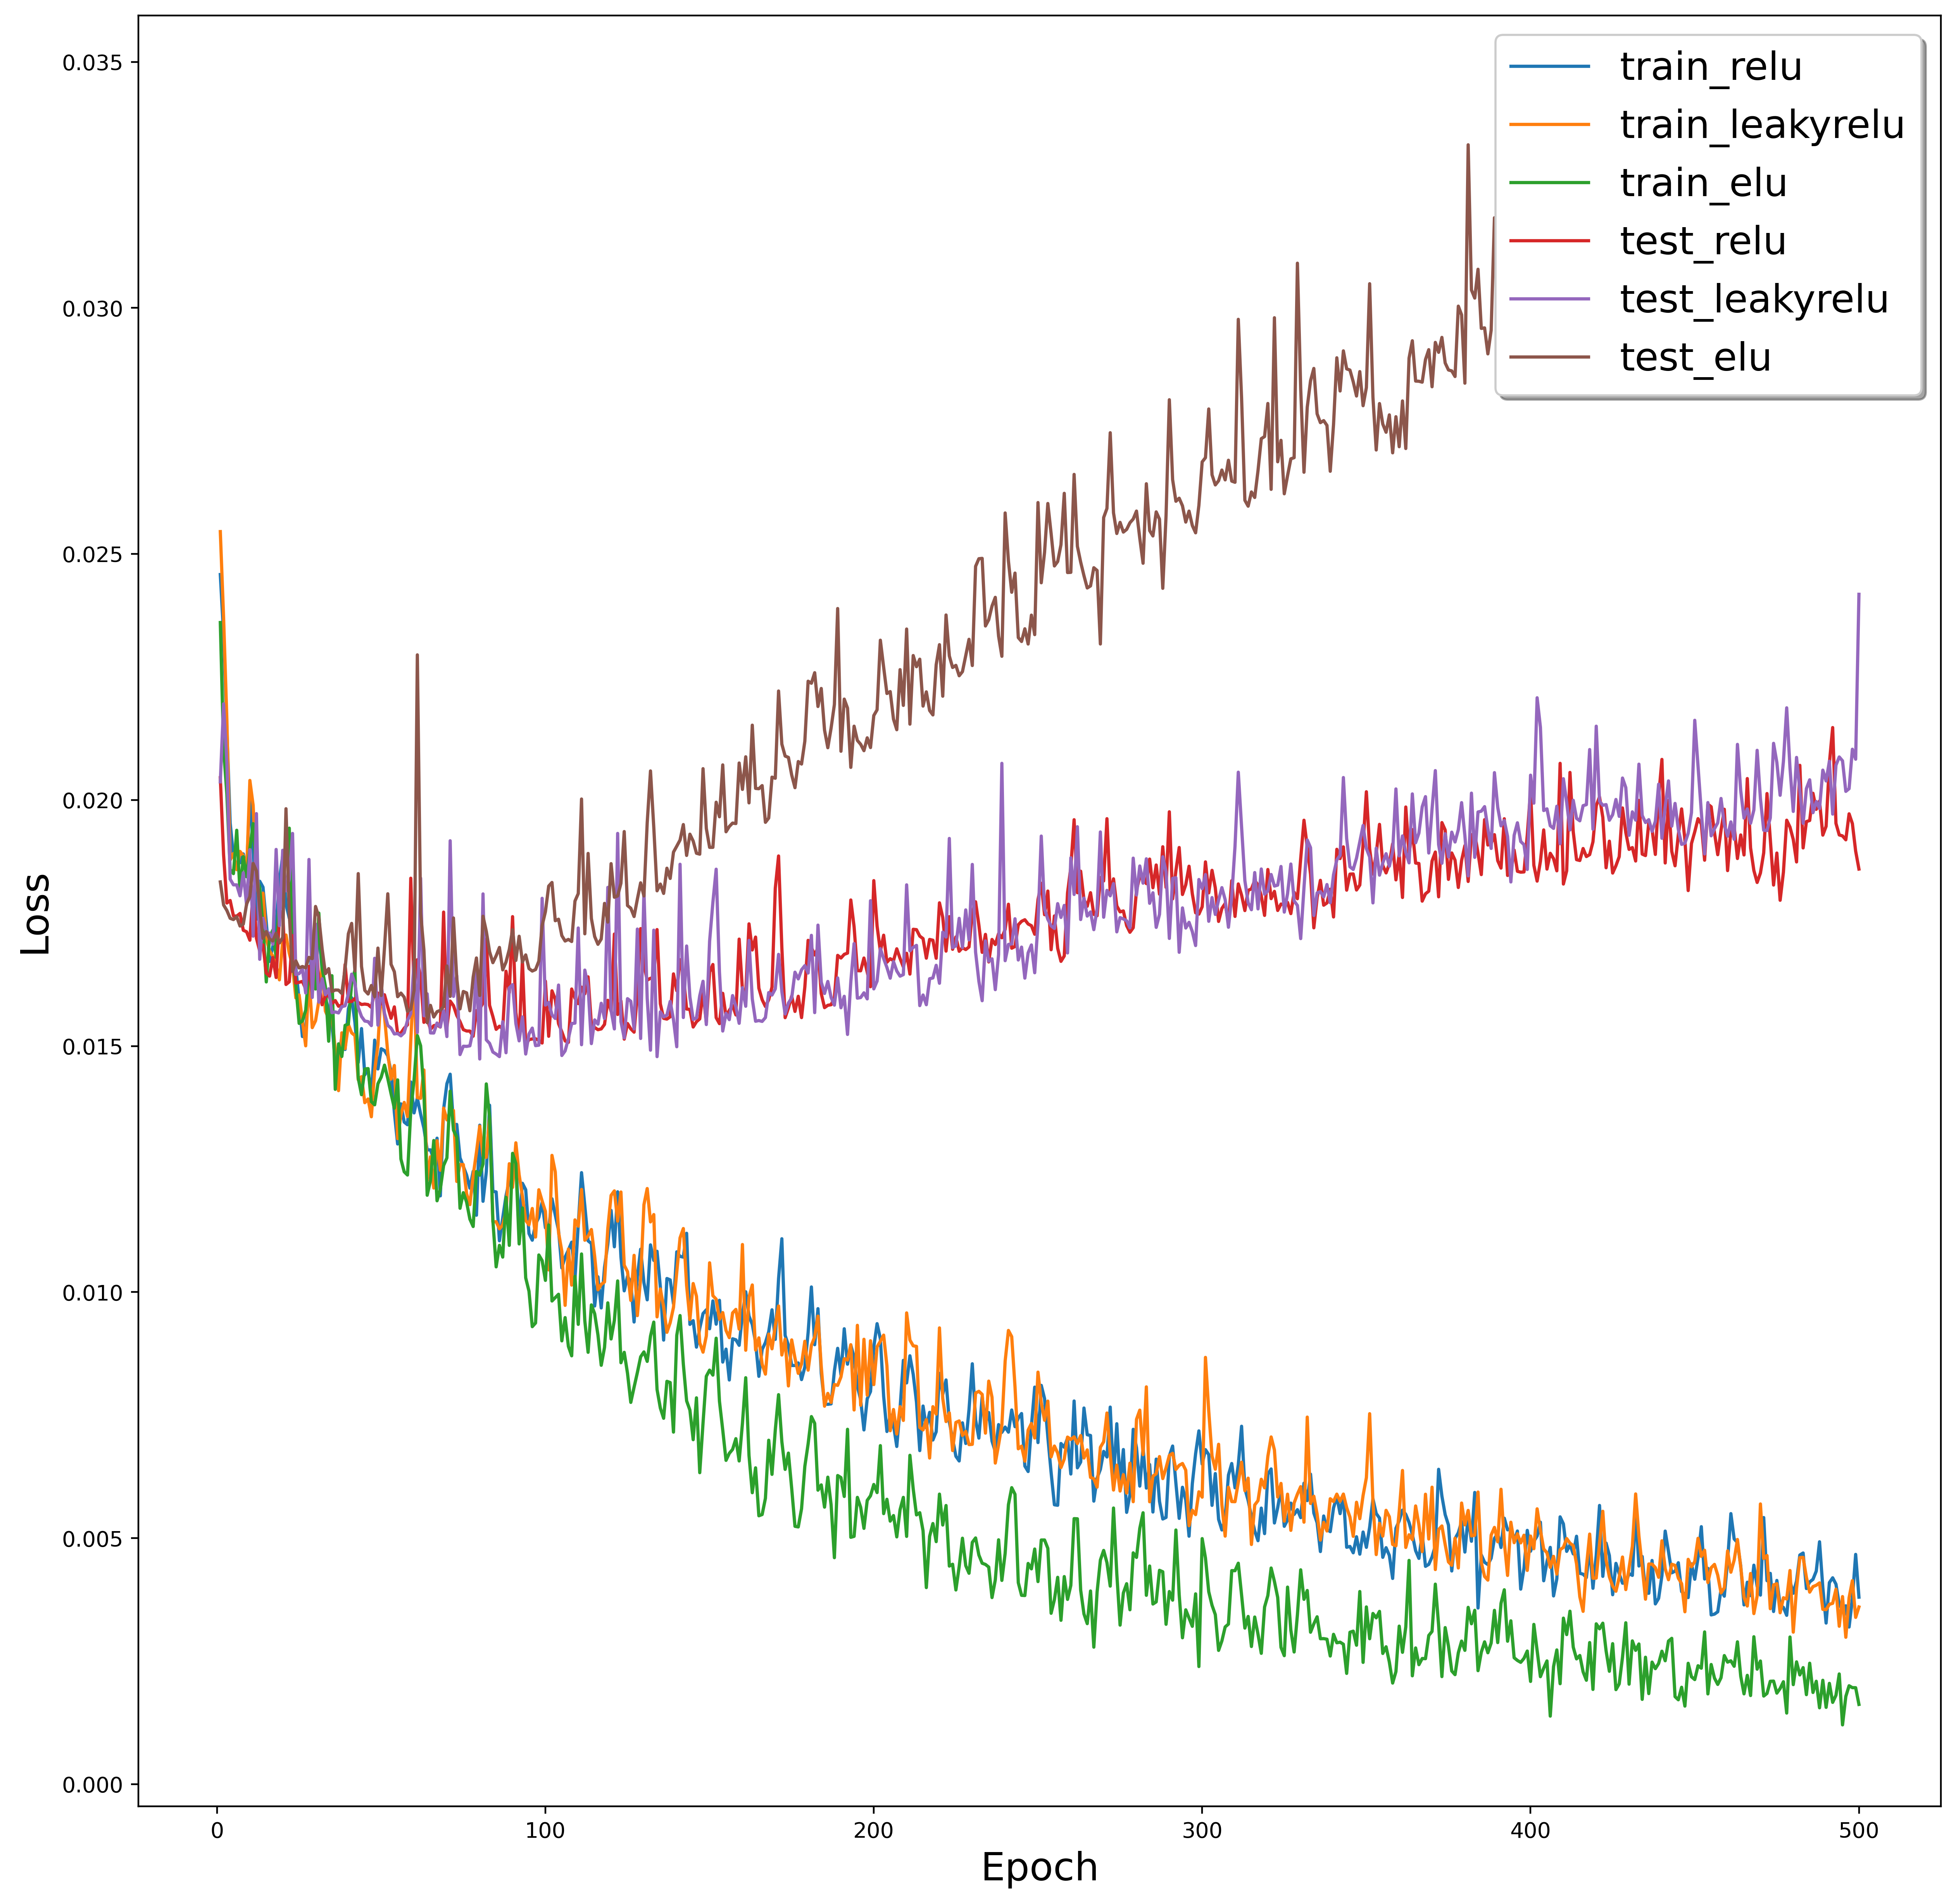
\includegraphics[width=0.45\textwidth]{results/deepconvnet_adam_32_0.0005_0.5_loss.png}
		\caption{DeepConvNet with Adam, 32 batch size, \\ $5 \times 10^{-4}$ learning rate, and 50\% dropout.}
	\end{figure}
	\begin{figure}[H]
		\centering
		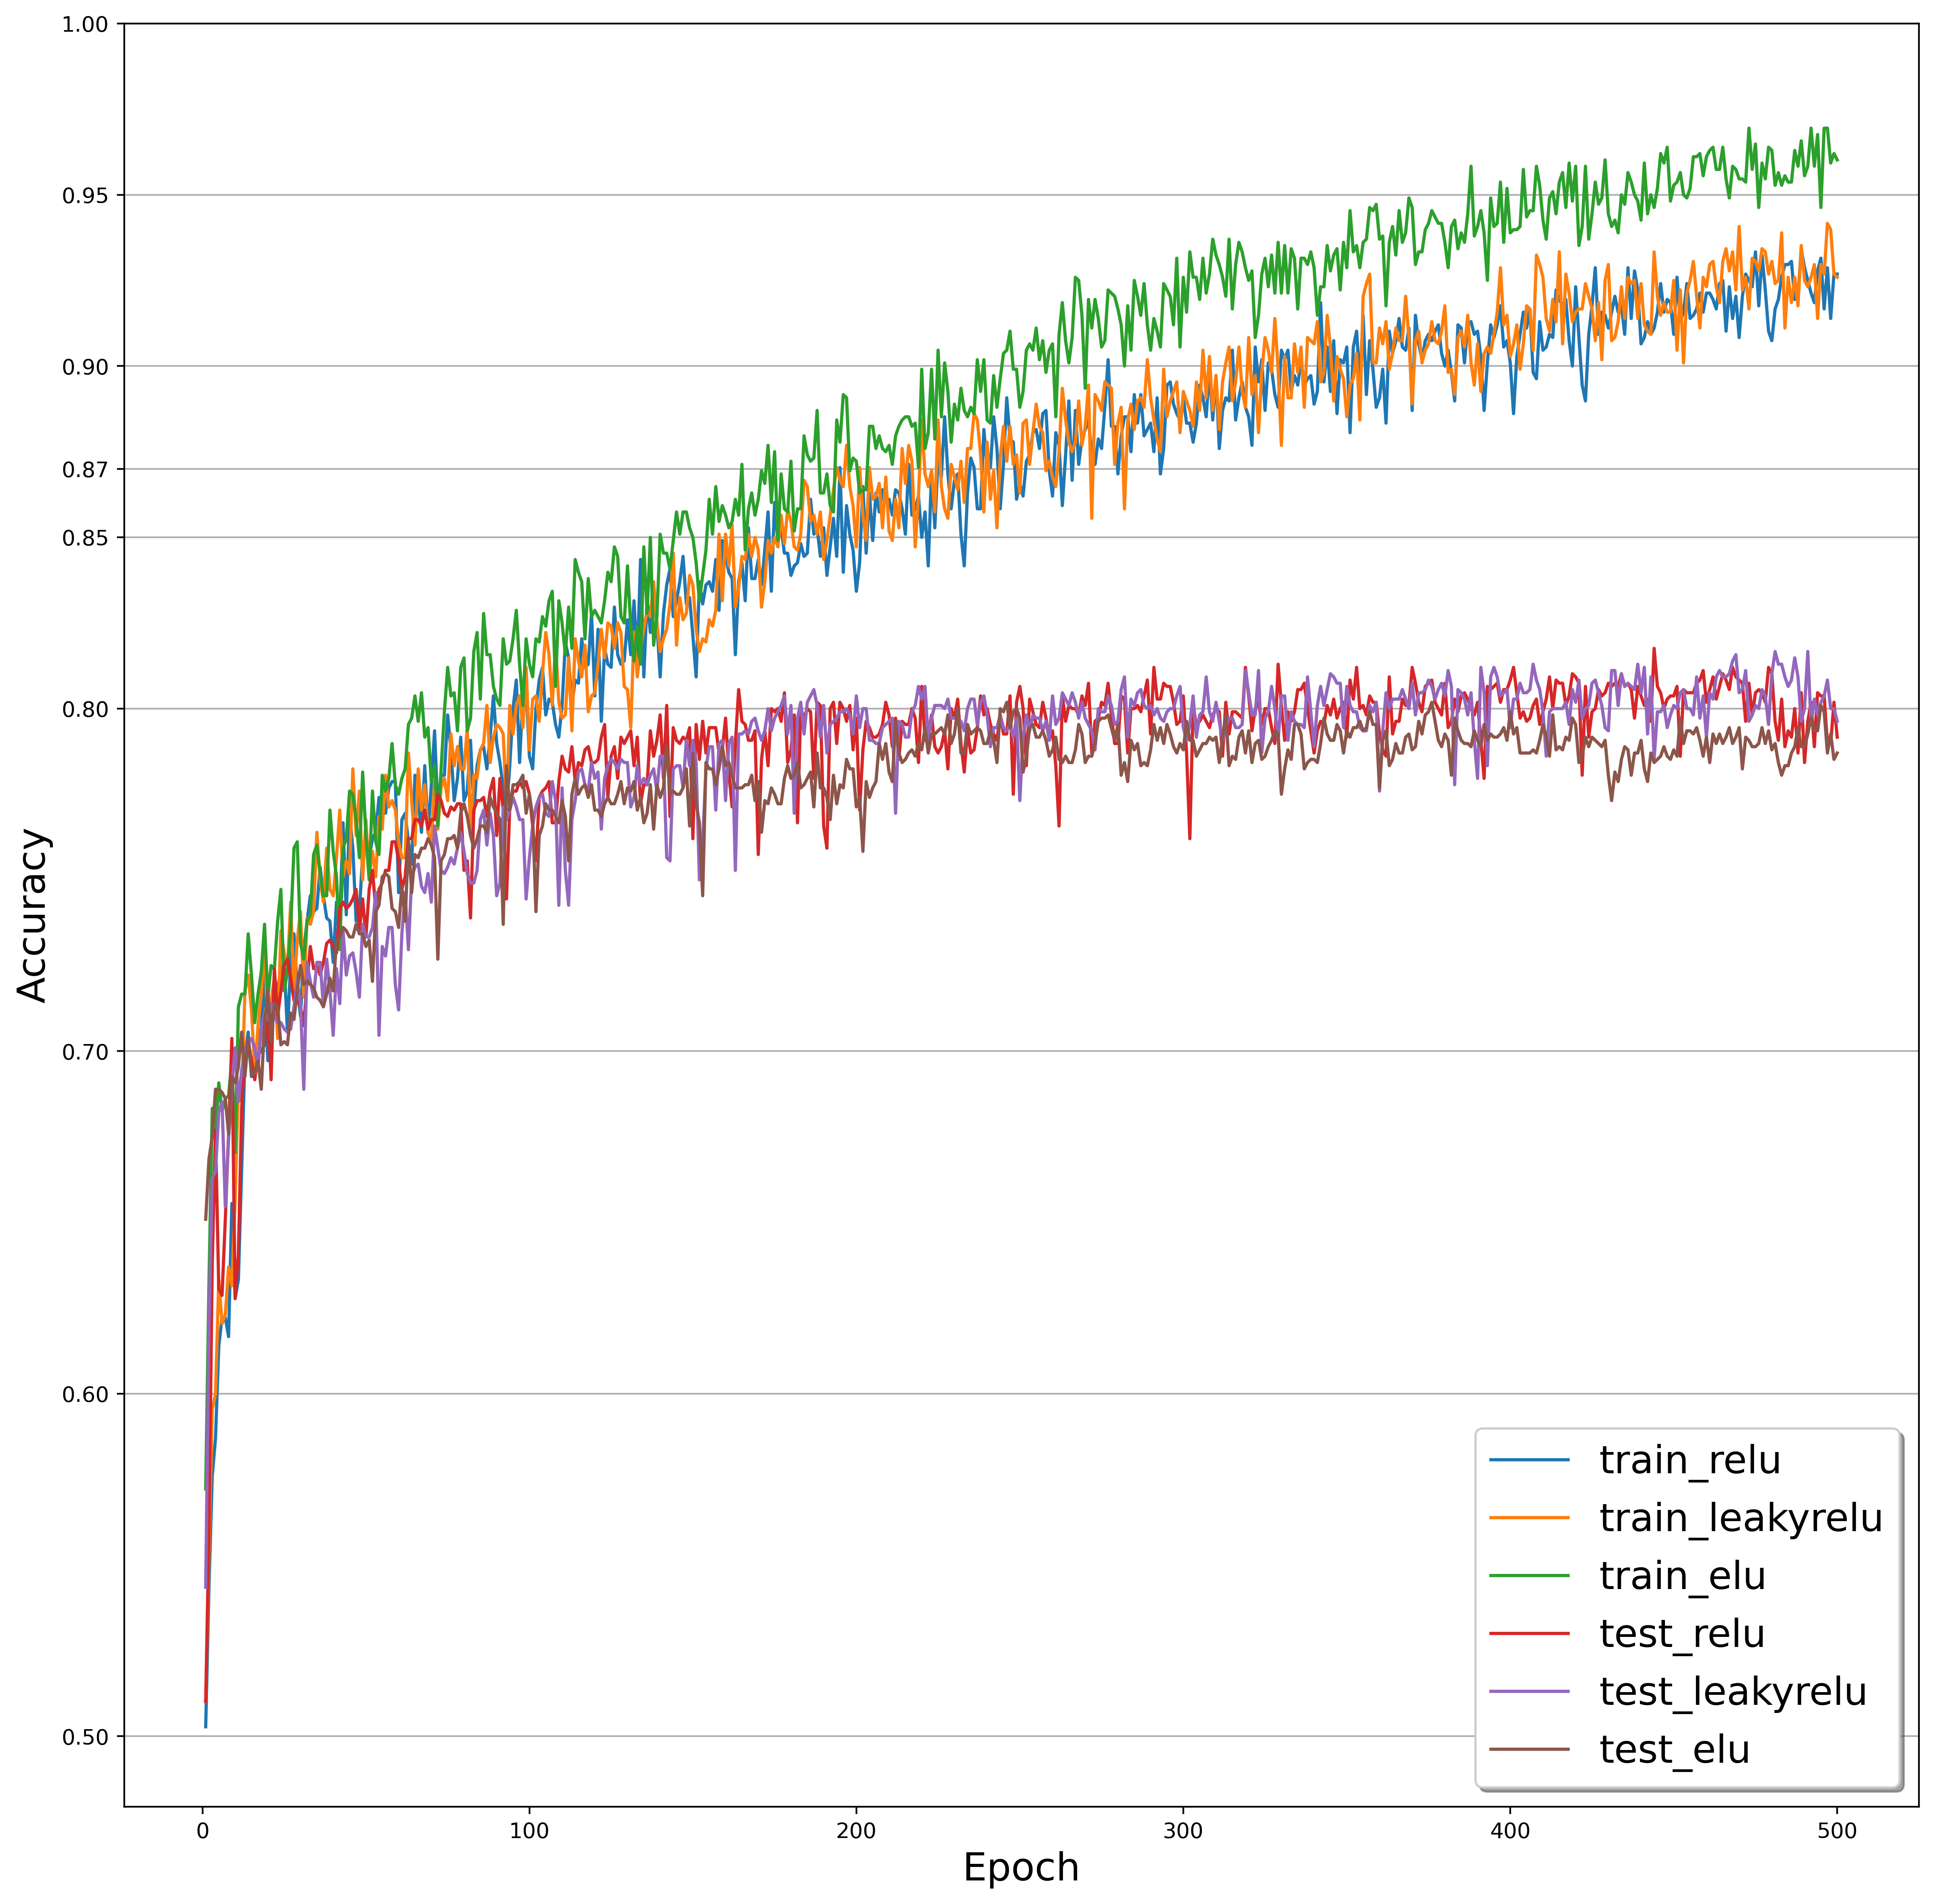
\includegraphics[width=0.45\textwidth]{results/deepconvnet_adam_128_0.0005_0.5_acc.png}
		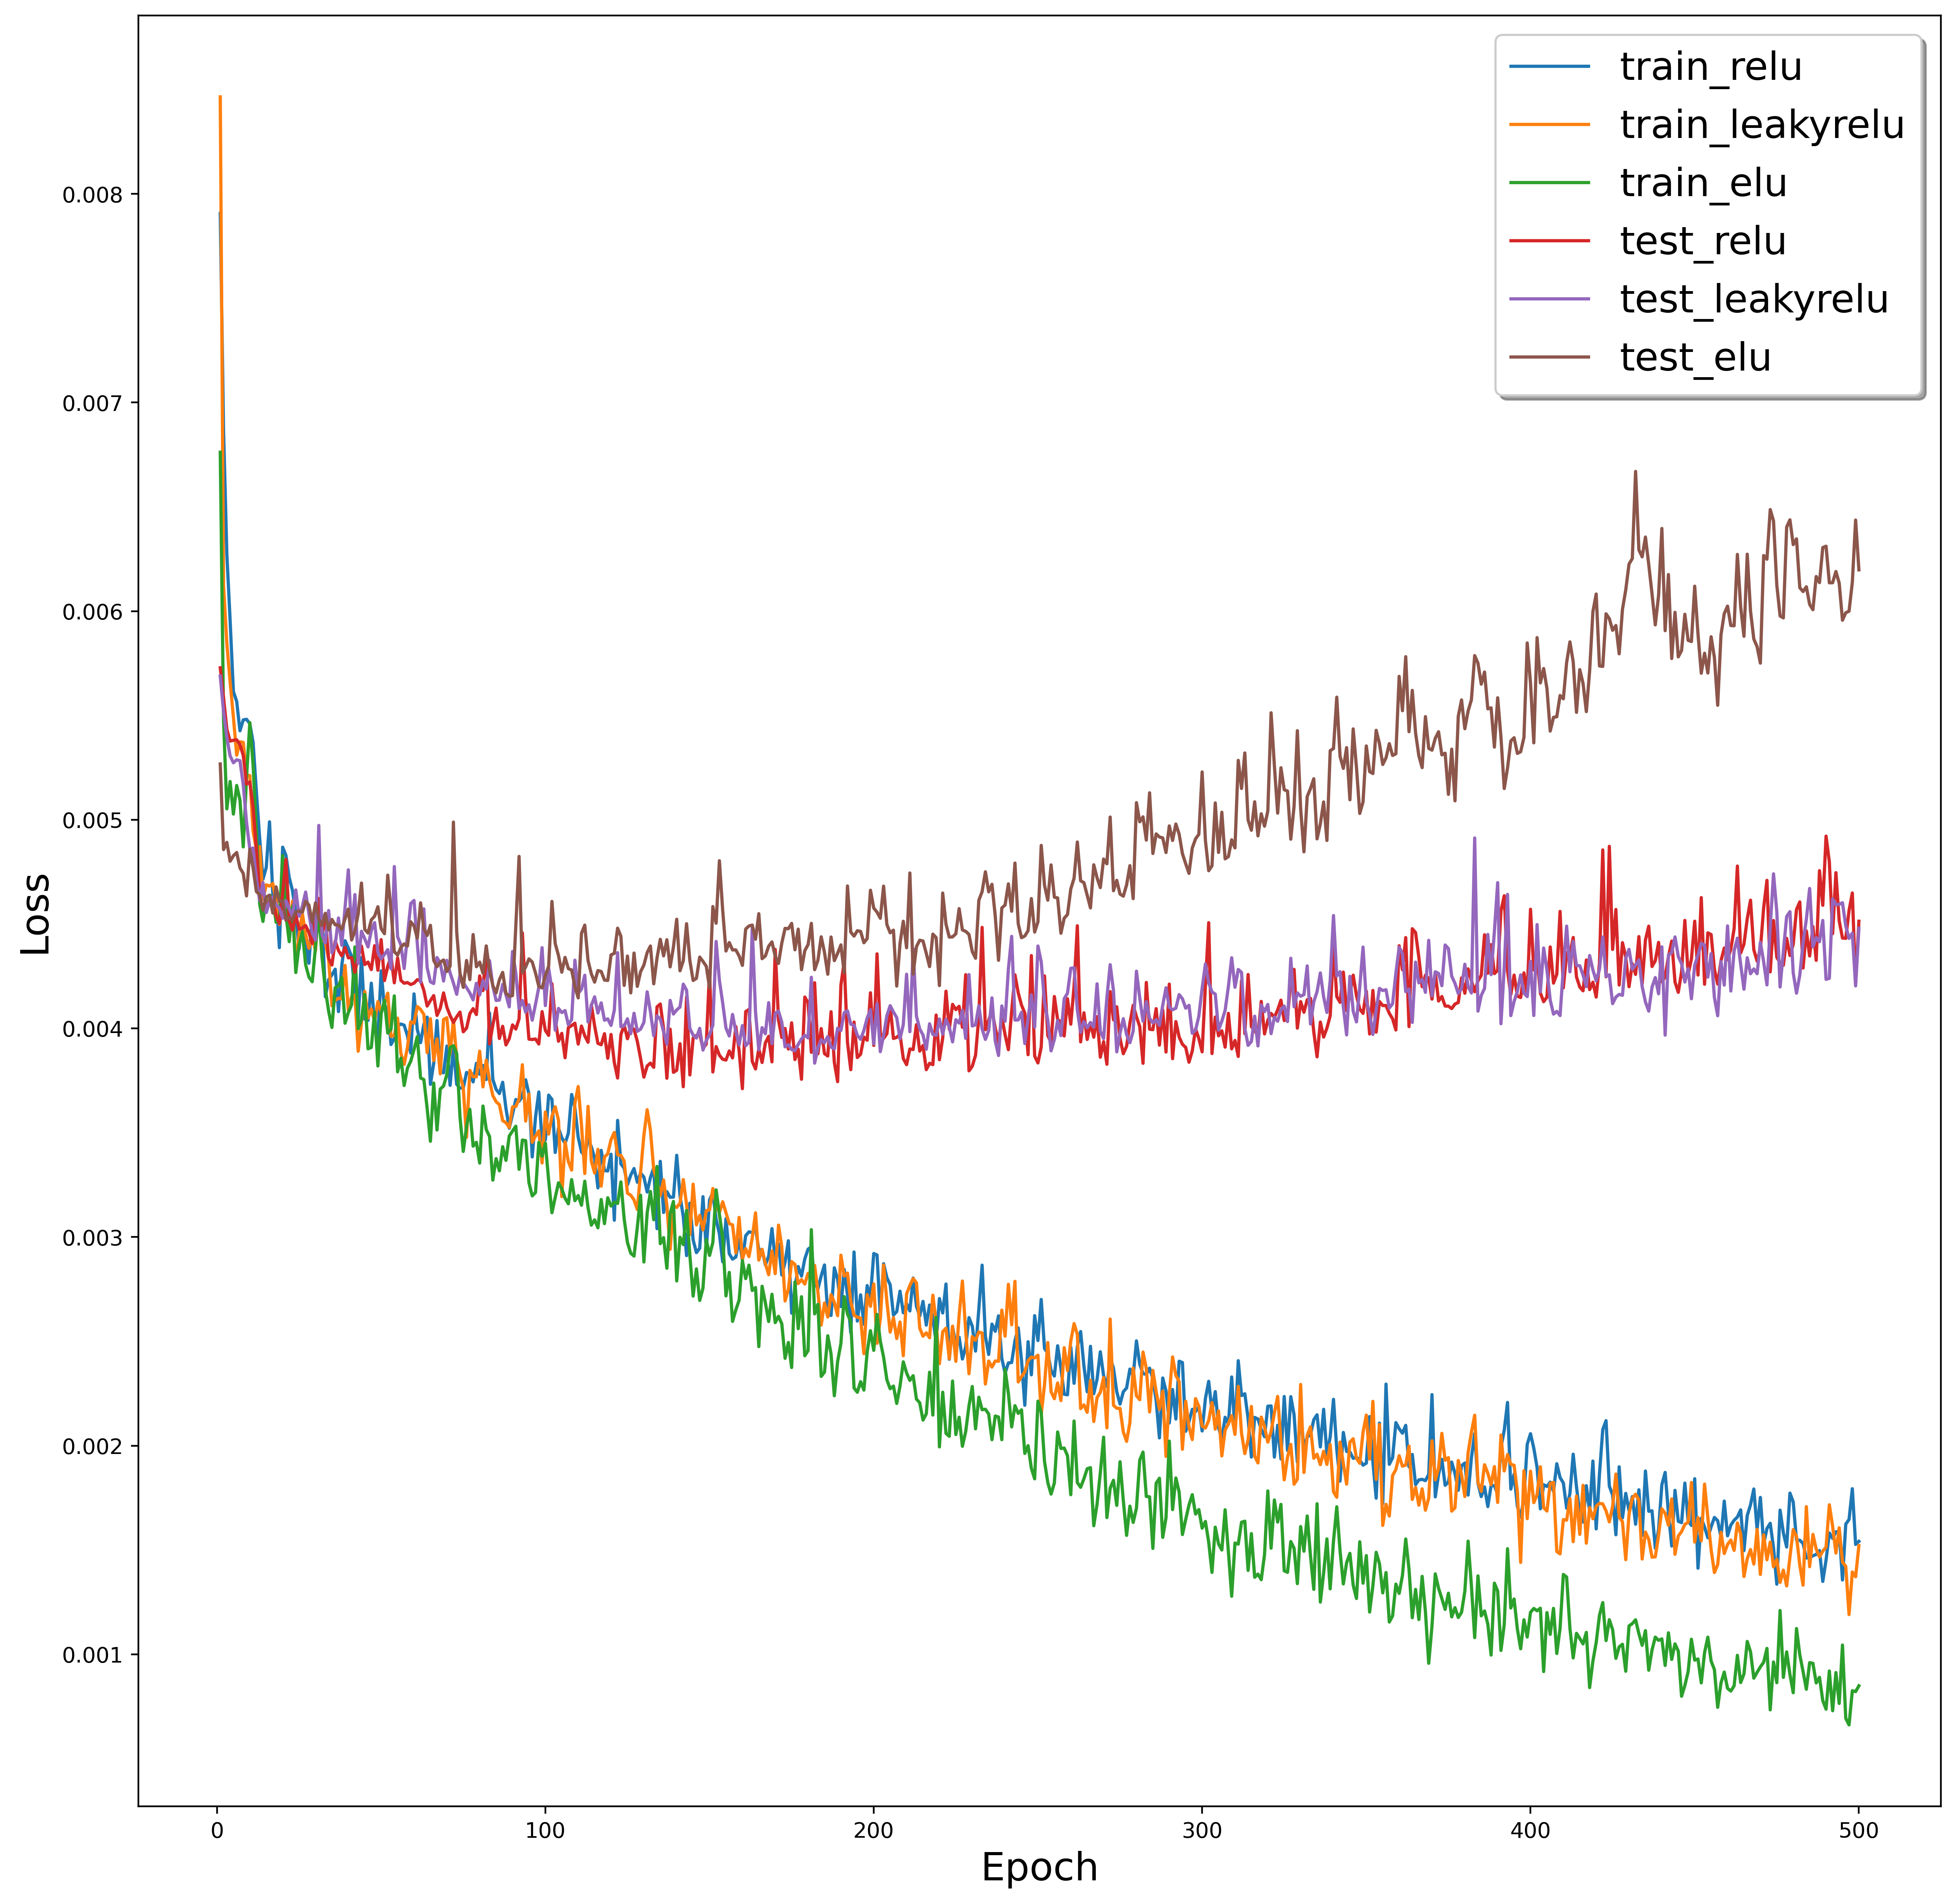
\includegraphics[width=0.45\textwidth]{results/deepconvnet_adam_128_0.0005_0.5_loss.png}
		\caption{DeepConvNet with Adam, 128 batch size, \\ $5 \times 10^{-4}$ learning rate, and 50\% dropout.}
	\end{figure}
	\begin{figure}[H]
		\centering
		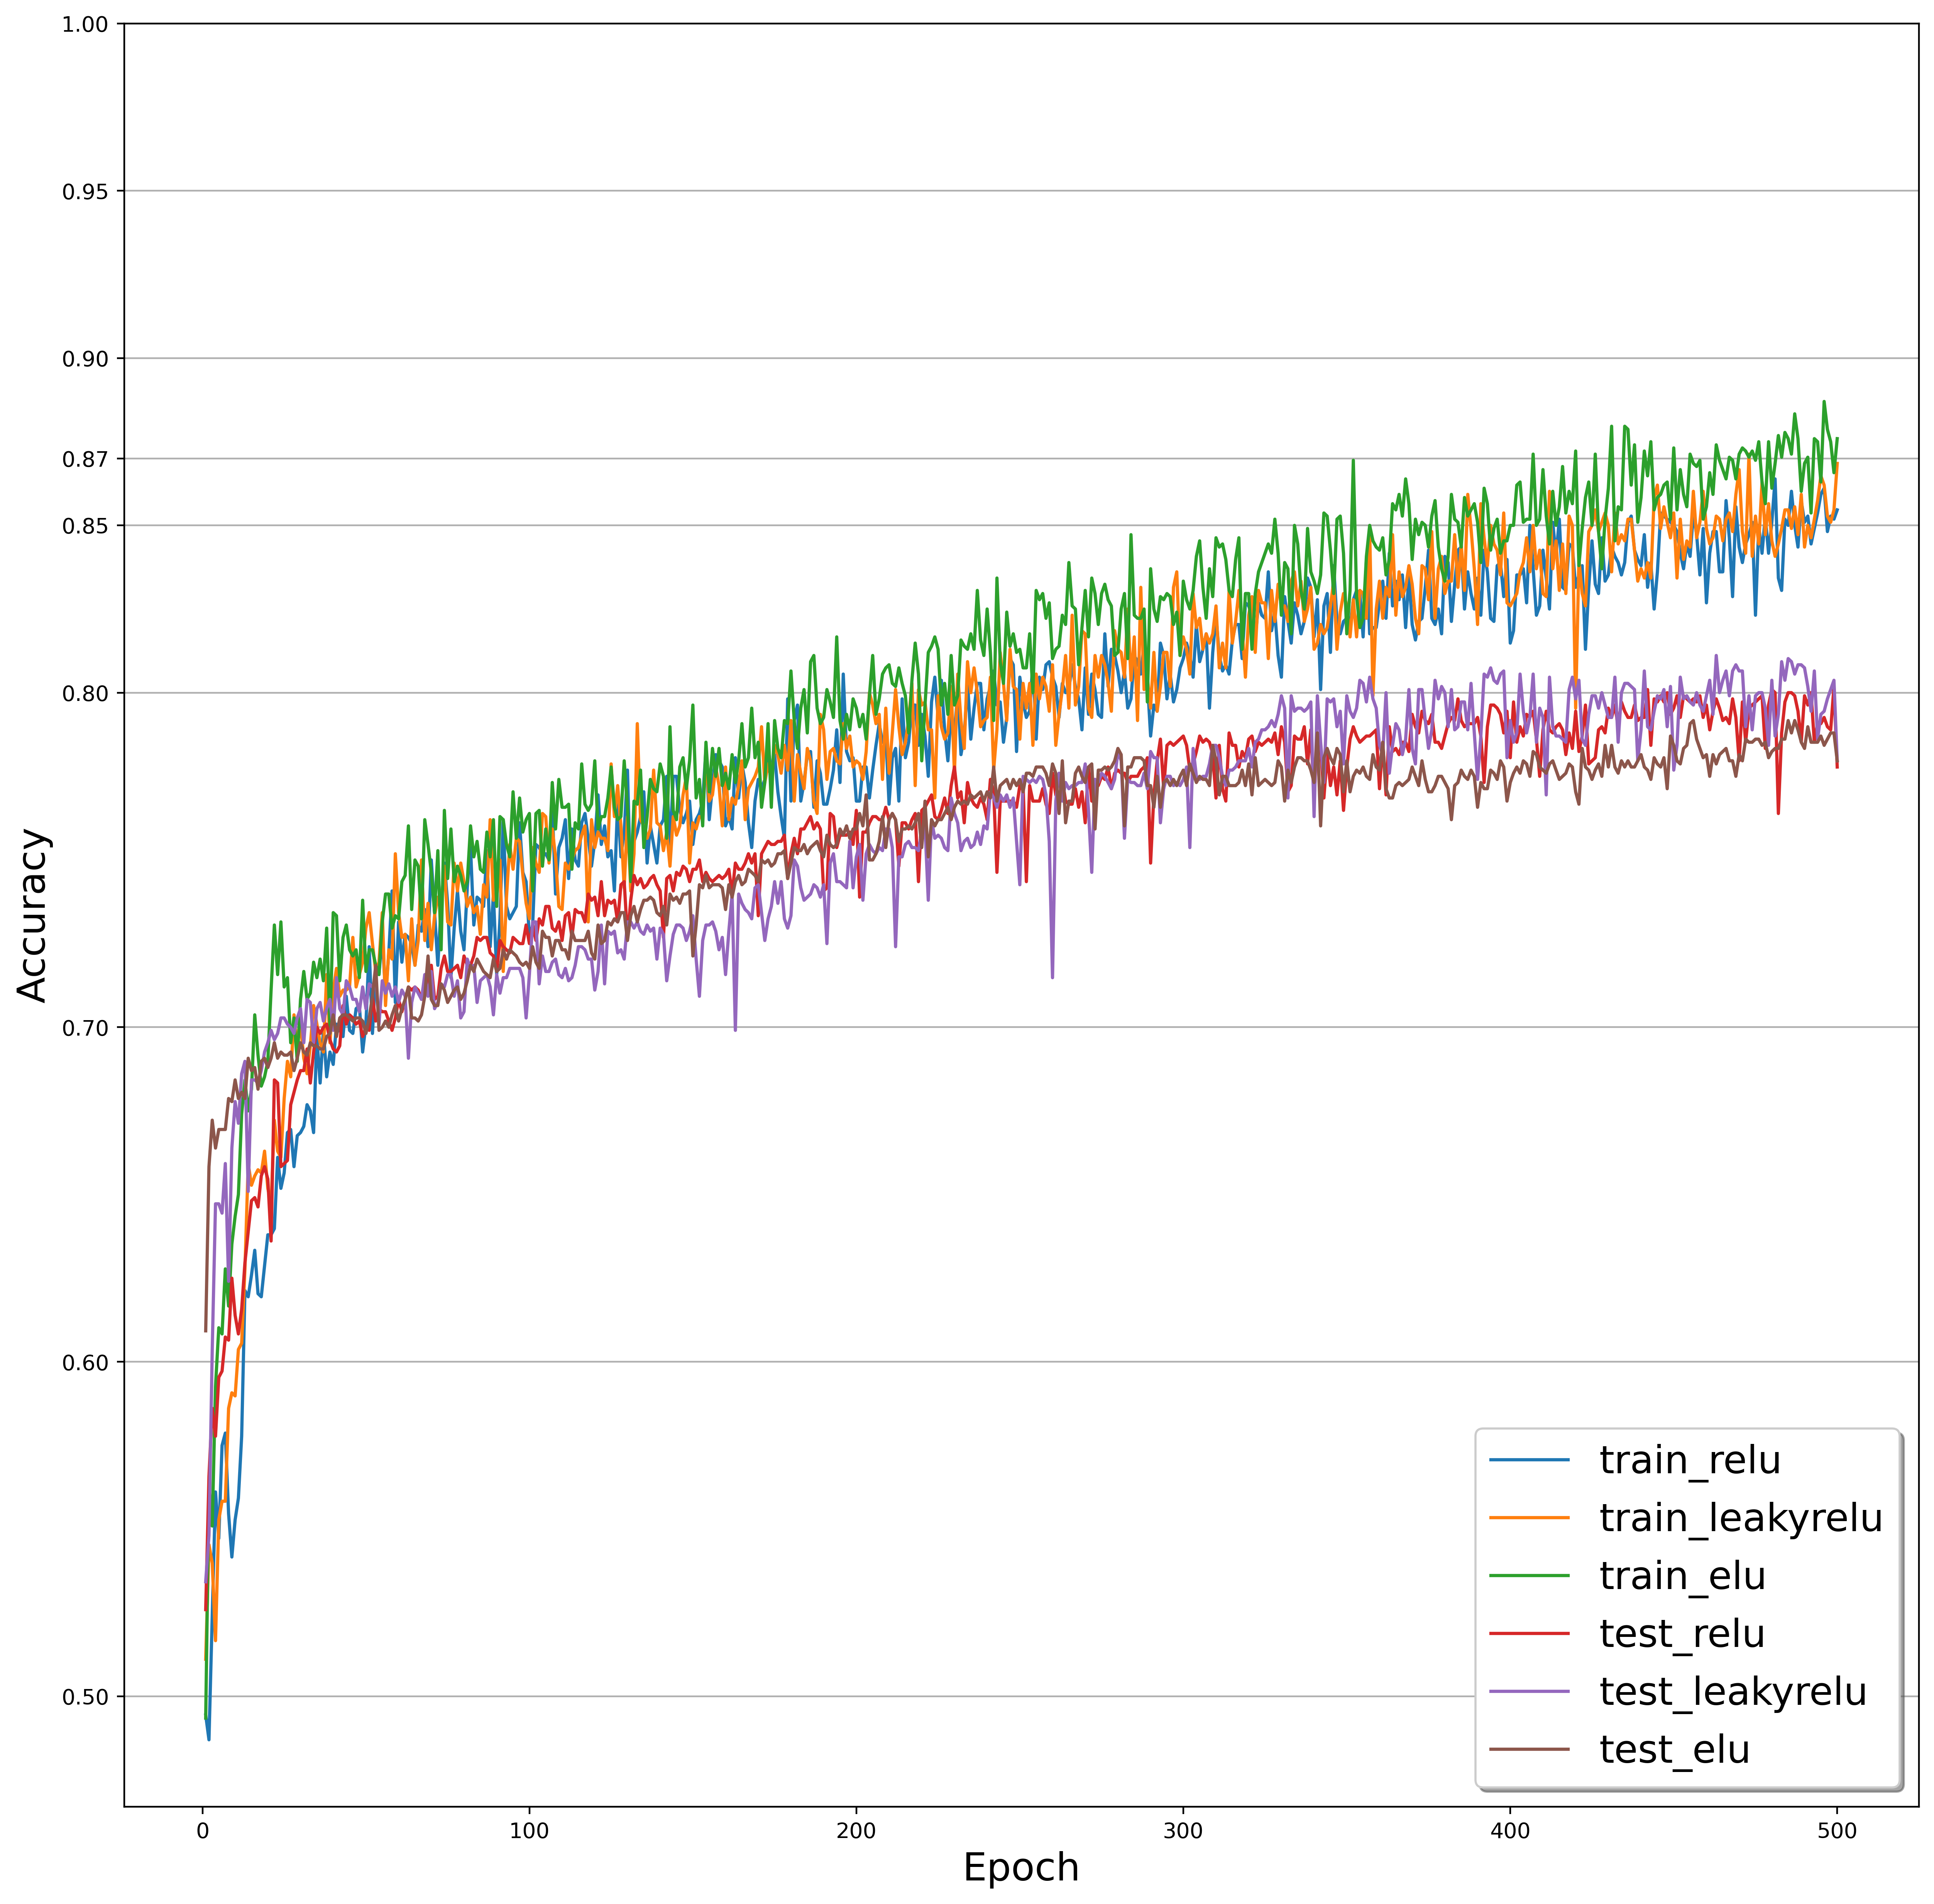
\includegraphics[width=0.45\textwidth]{results/deepconvnet_adam_64_0.0001_0.5_acc.png}
		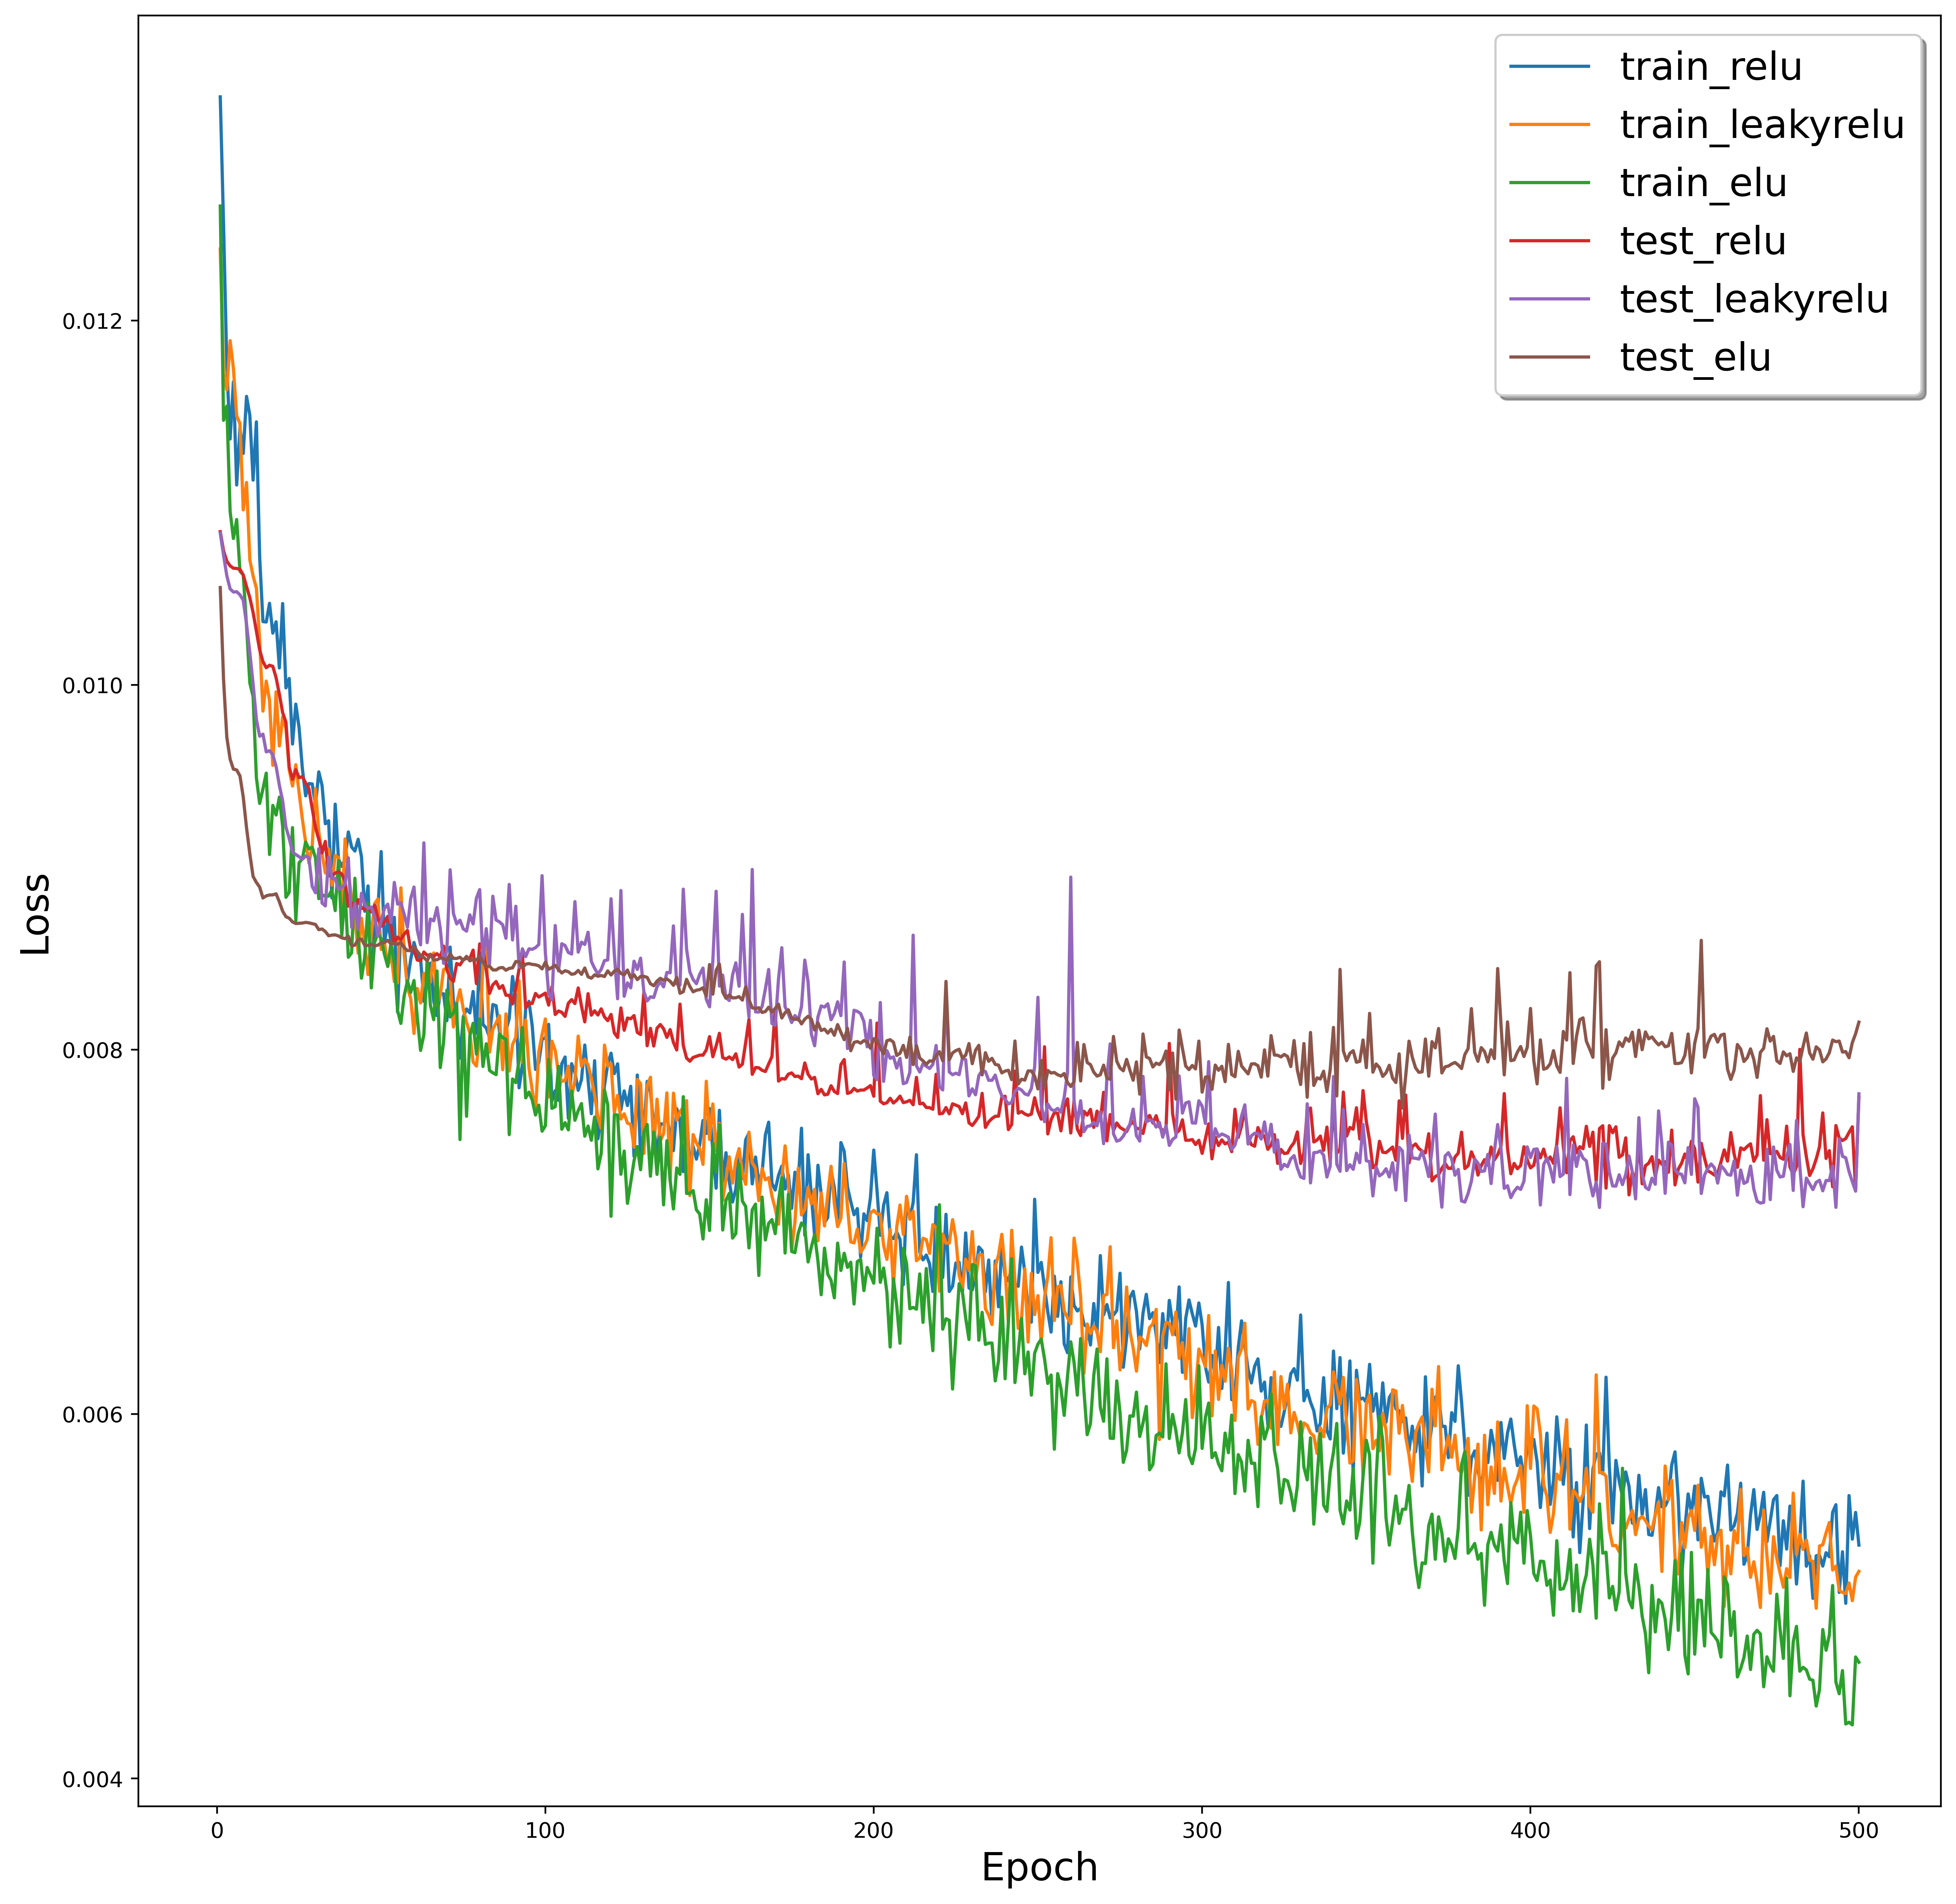
\includegraphics[width=0.45\textwidth]{results/deepconvnet_adam_64_0.0001_0.5_loss.png}
		\caption{DeepConvNet with Adam, 64 batch size, \\ $1 \times 10^{-4}$ learning rate, and 50\% dropout.}
	\end{figure}
	\begin{figure}[H]
		\centering
		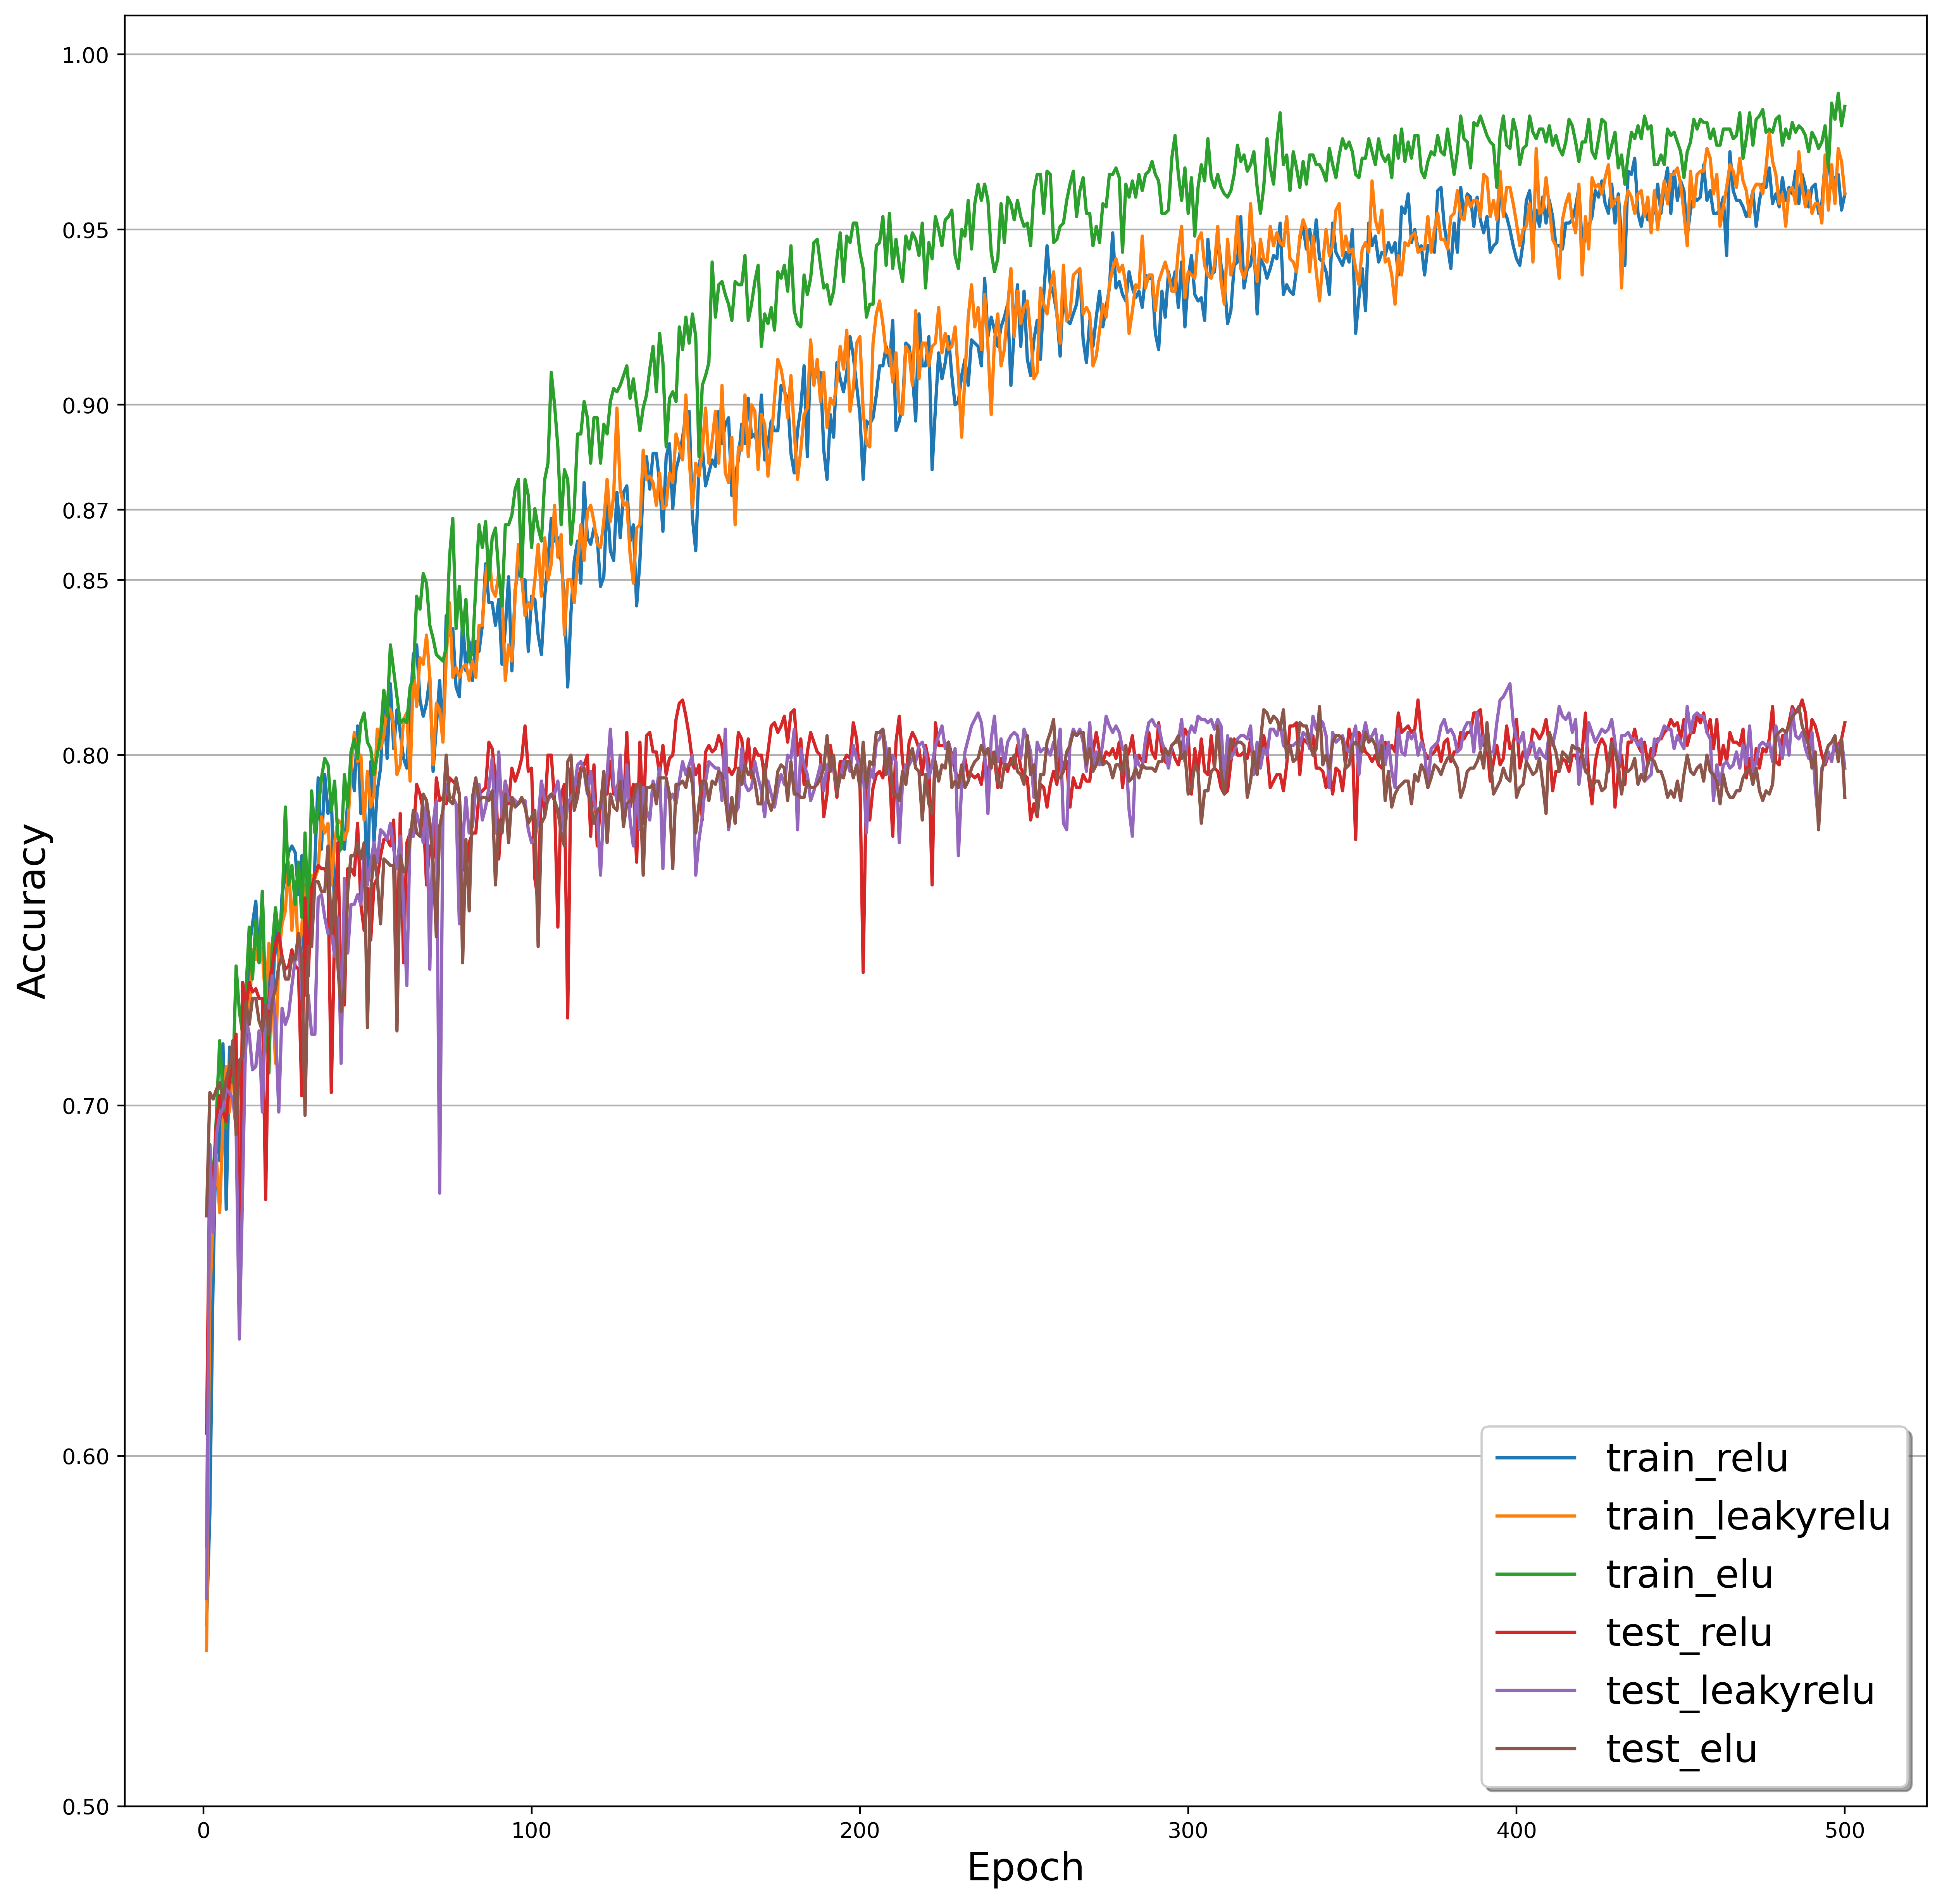
\includegraphics[width=0.45\textwidth]{results/deepconvnet_adam_64_0.001_0.5_acc.png}
		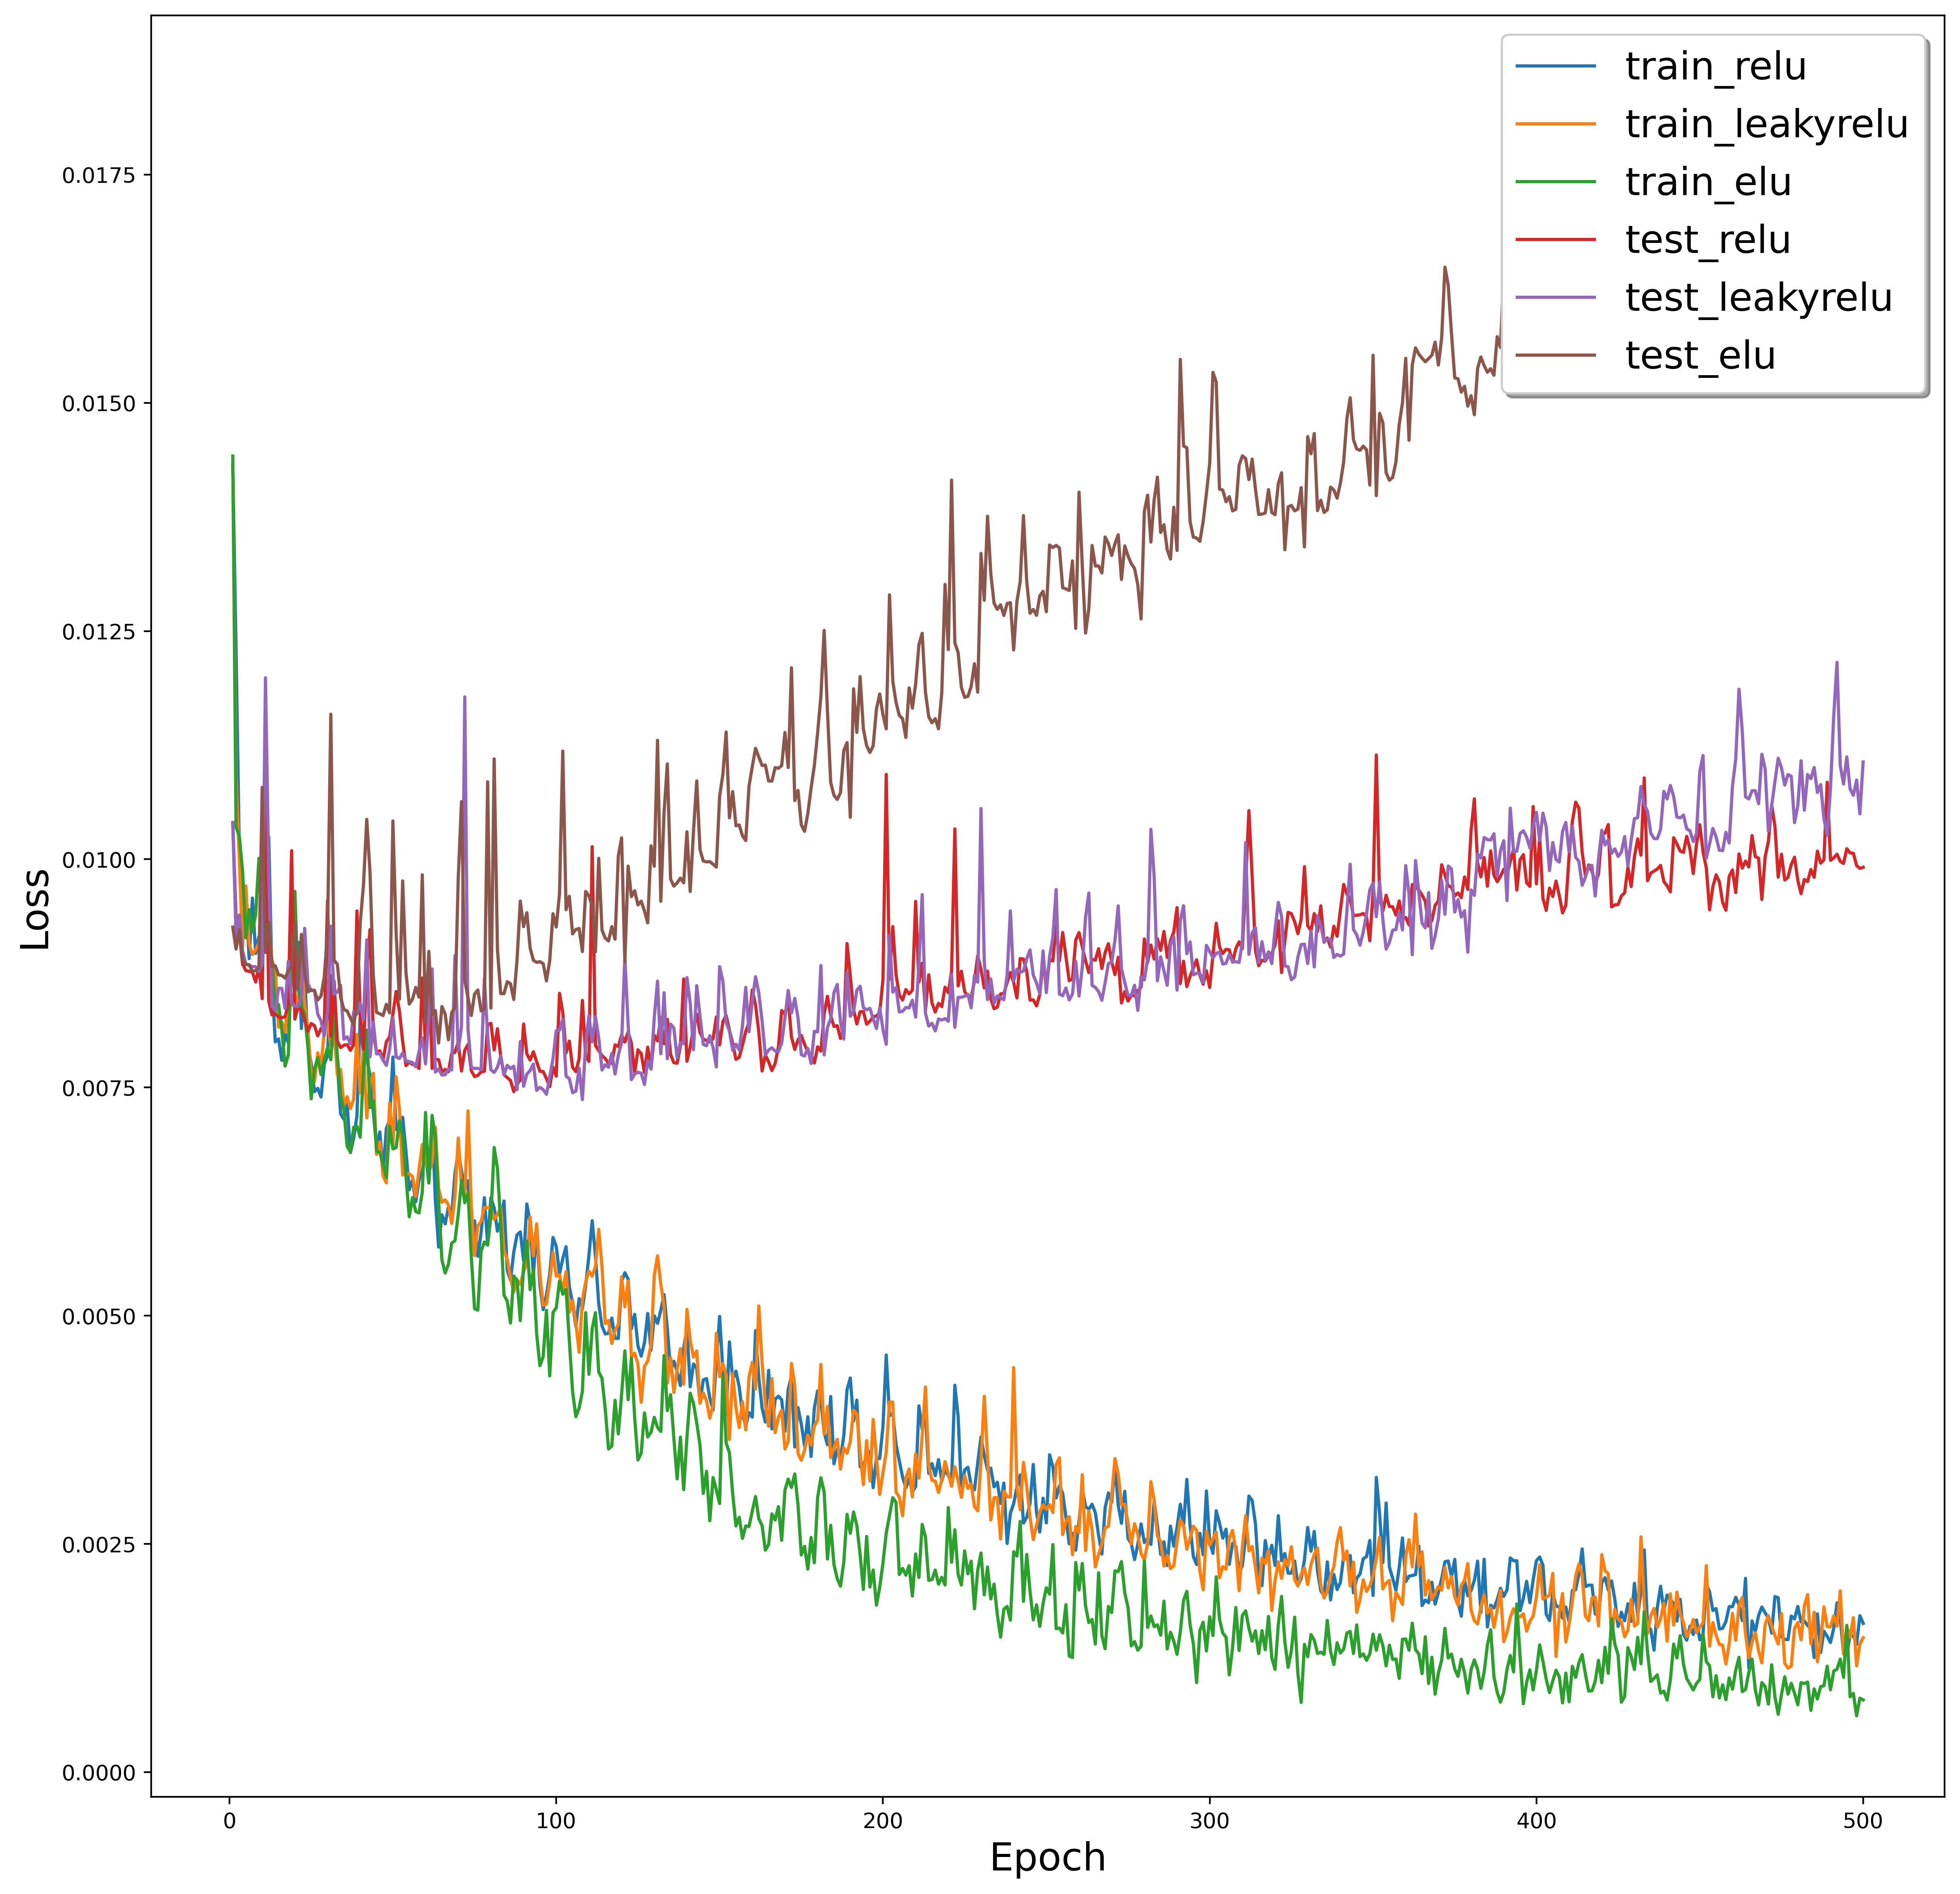
\includegraphics[width=0.45\textwidth]{results/deepconvnet_adam_64_0.001_0.5_loss.png}
		\caption{DeepConvNet with Adam, 64 batch size, \\ $1 \times 10^{-3}$ learning rate, and 50\% dropout.}
	\end{figure}
	\begin{figure}[H]
		\centering
		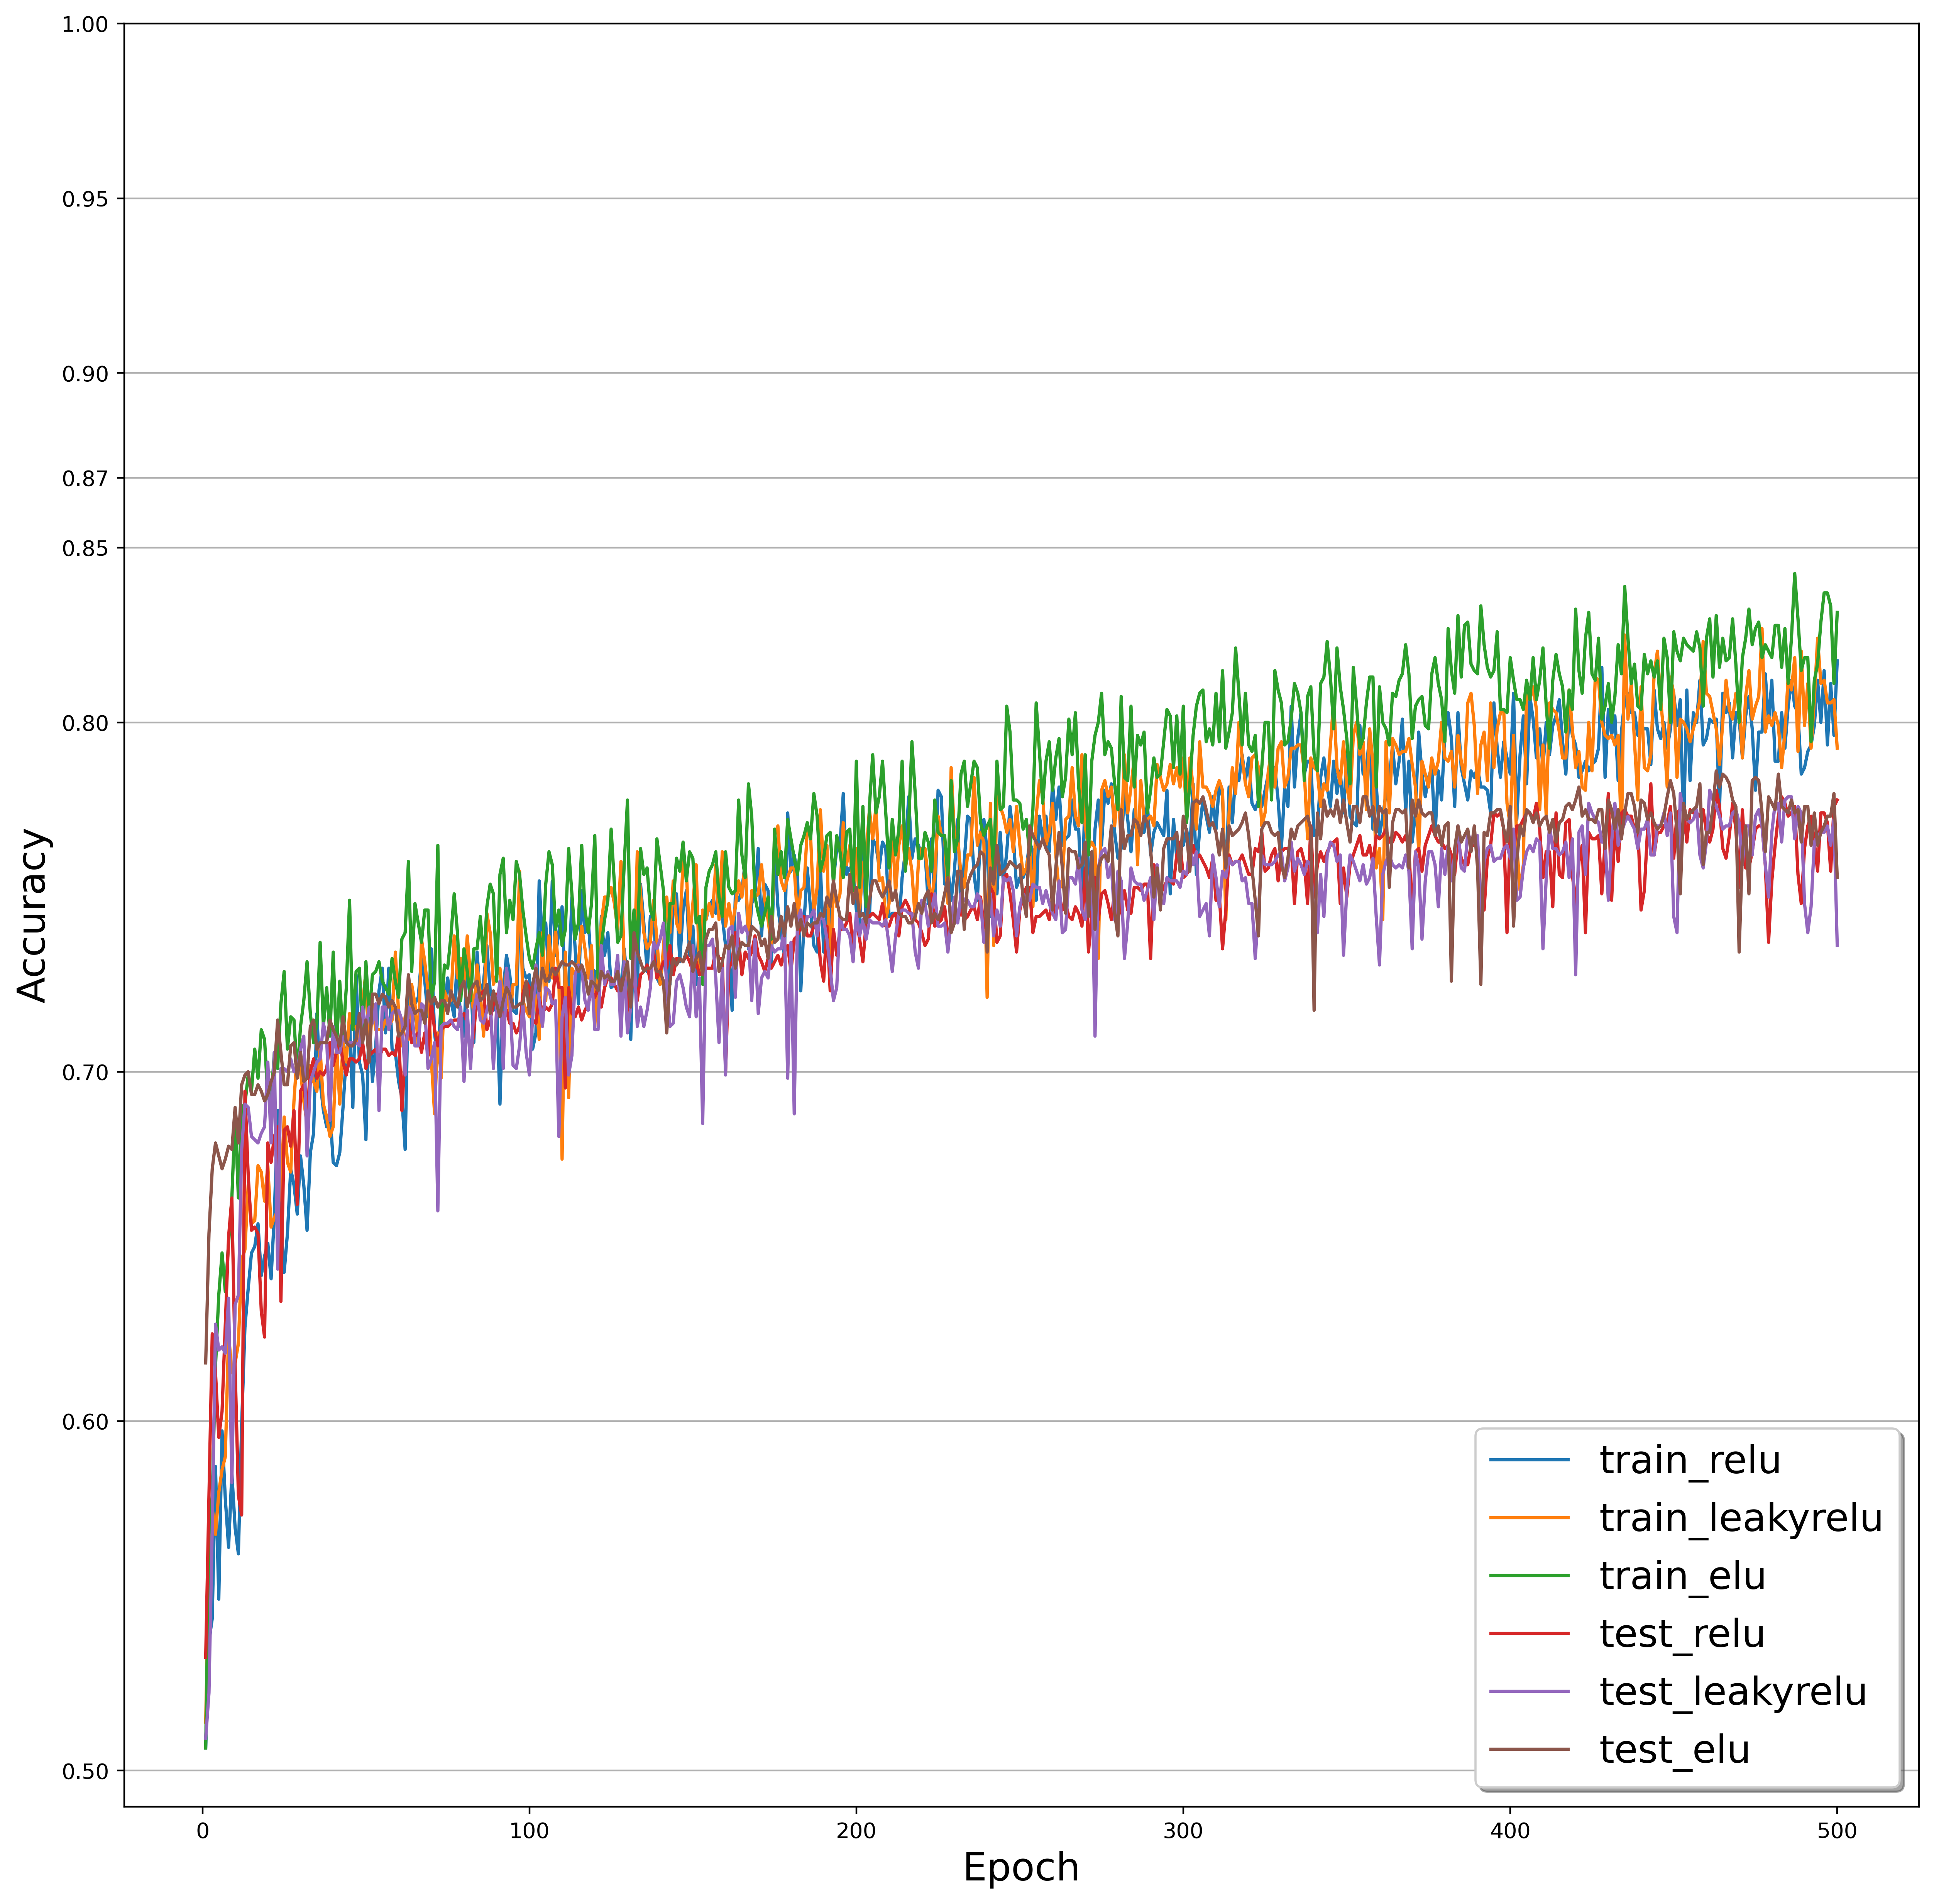
\includegraphics[width=0.45\textwidth]{results/deepconvnet_sgd_64_0.0005_0.5_acc.png}
		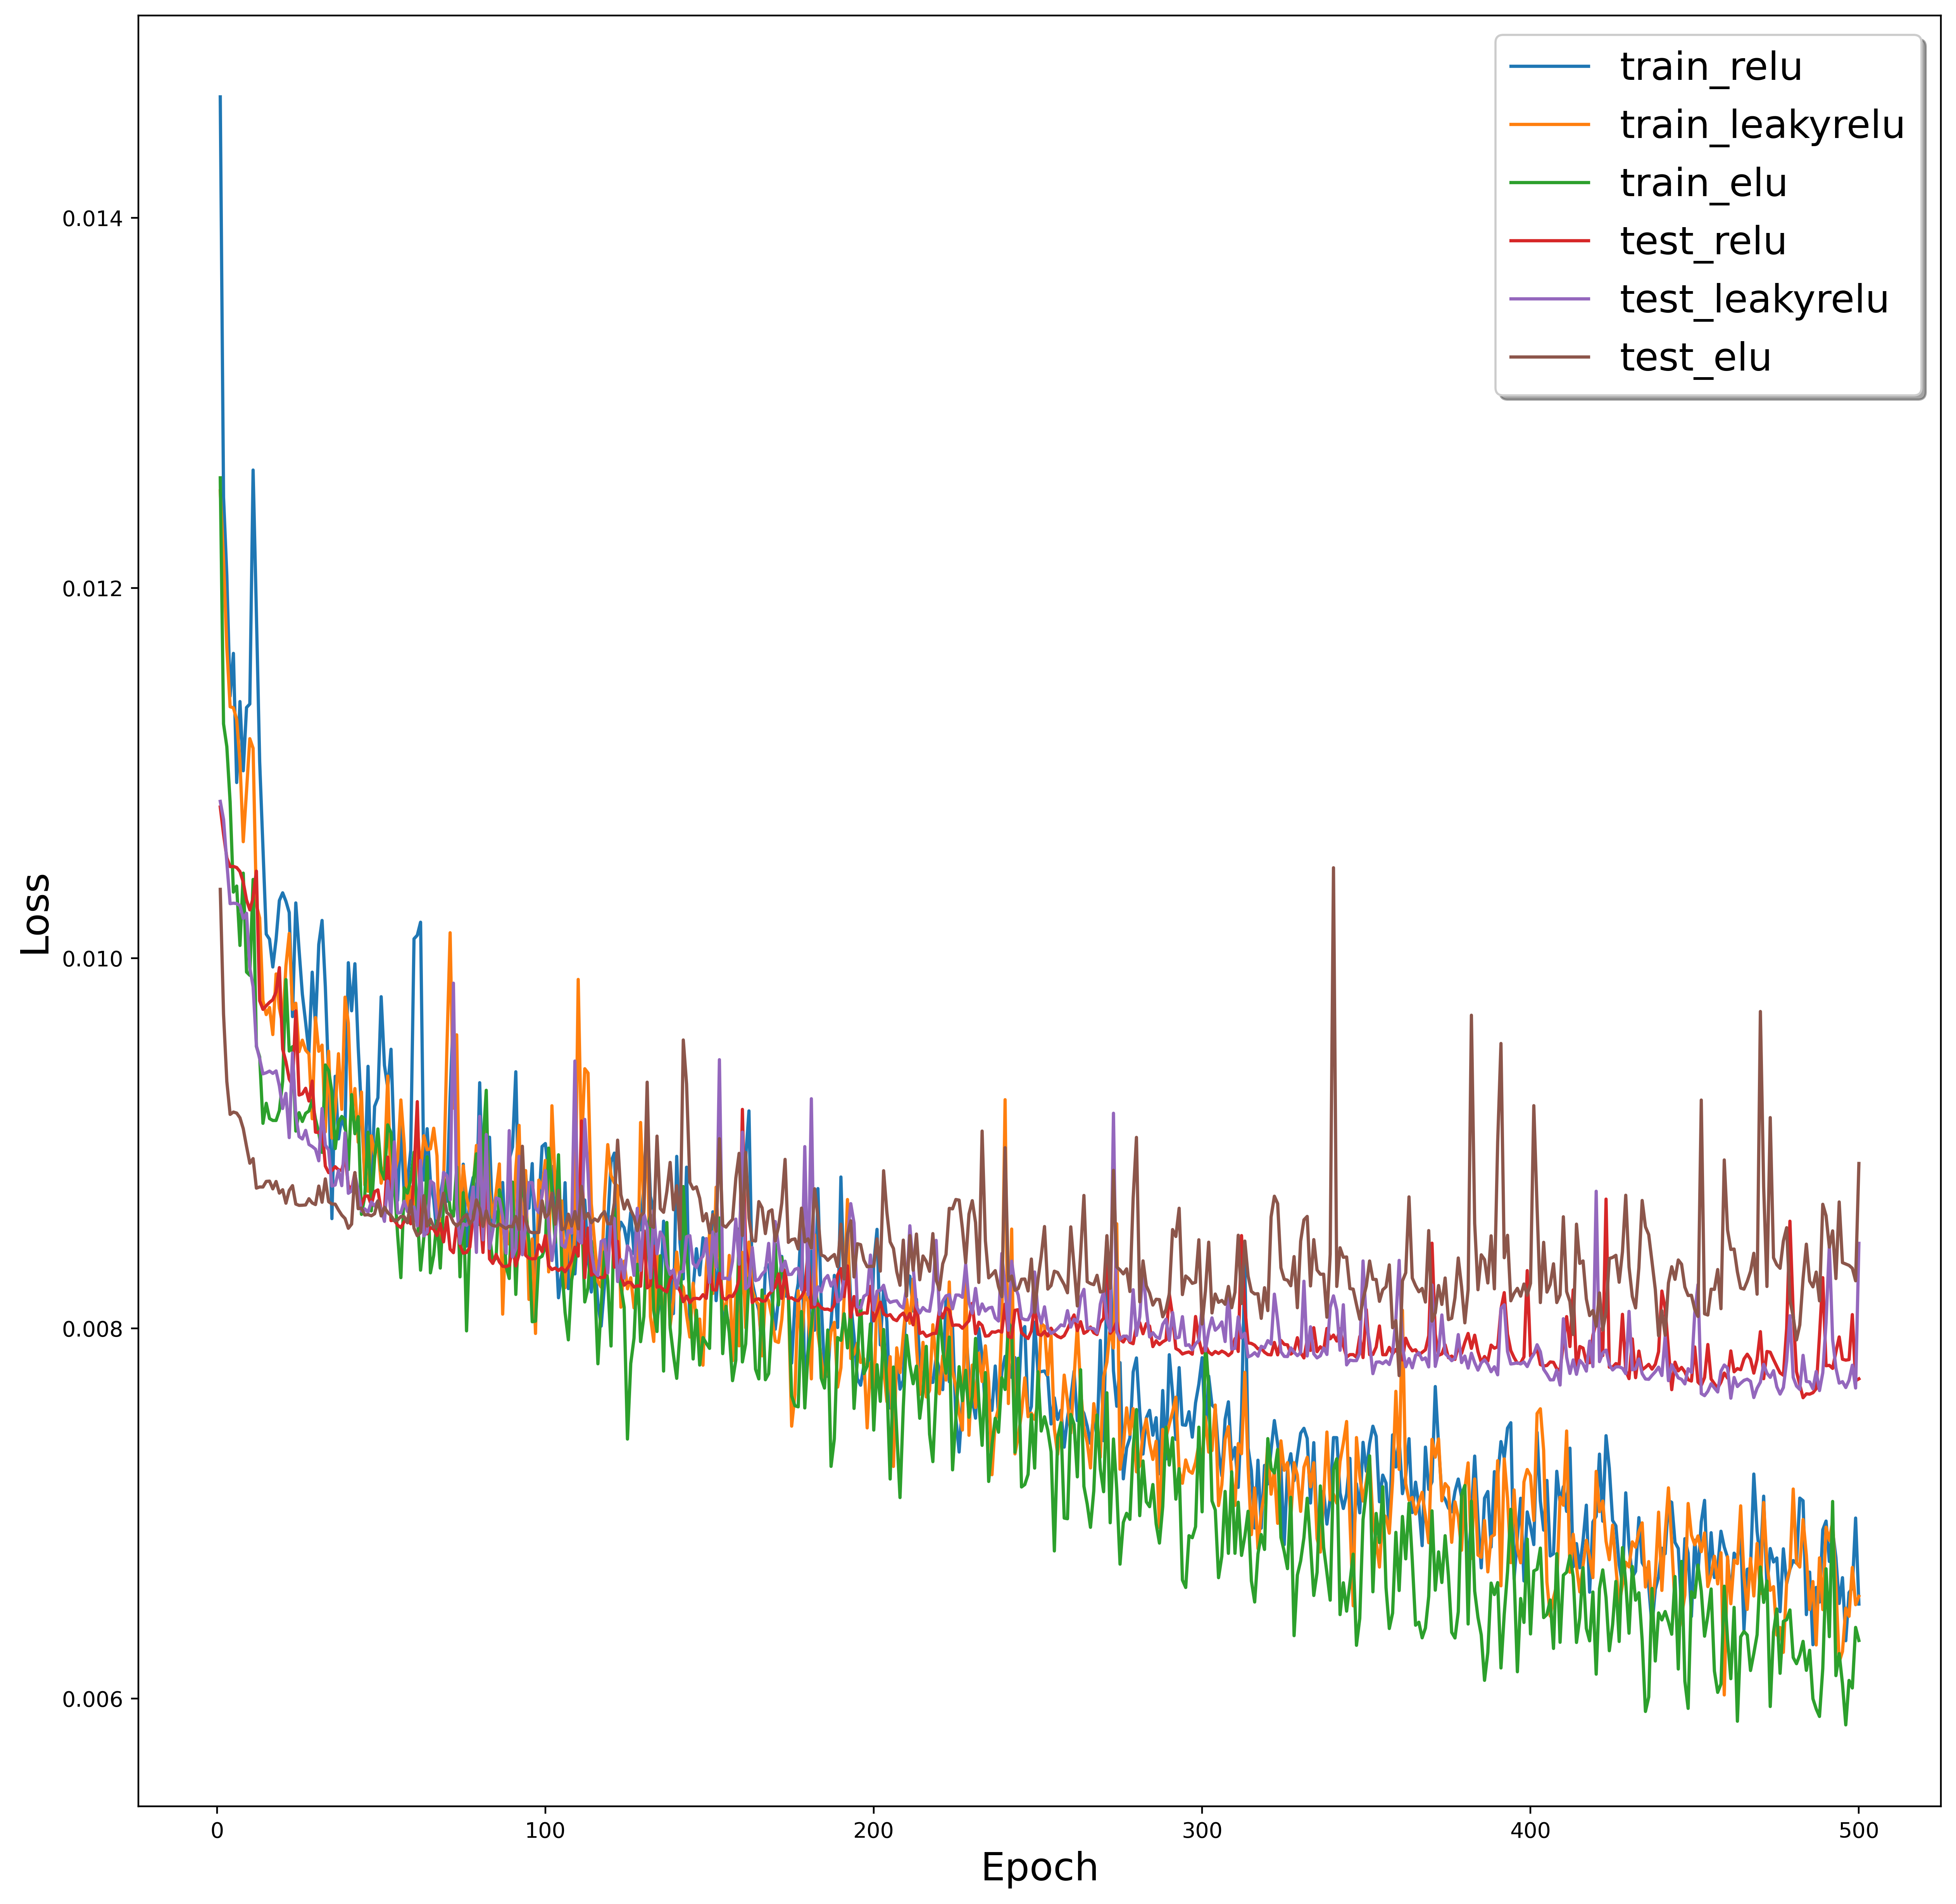
\includegraphics[width=0.45\textwidth]{results/deepconvnet_sgd_64_0.0005_0.5_loss.png}
		\caption{DeepConvNet with SGD, 64 batch size, \\ $5 \times 10^{-4}$ learning rate, and 50\% dropout.}
	\end{figure}
	\begin{figure}[H]
		\centering
		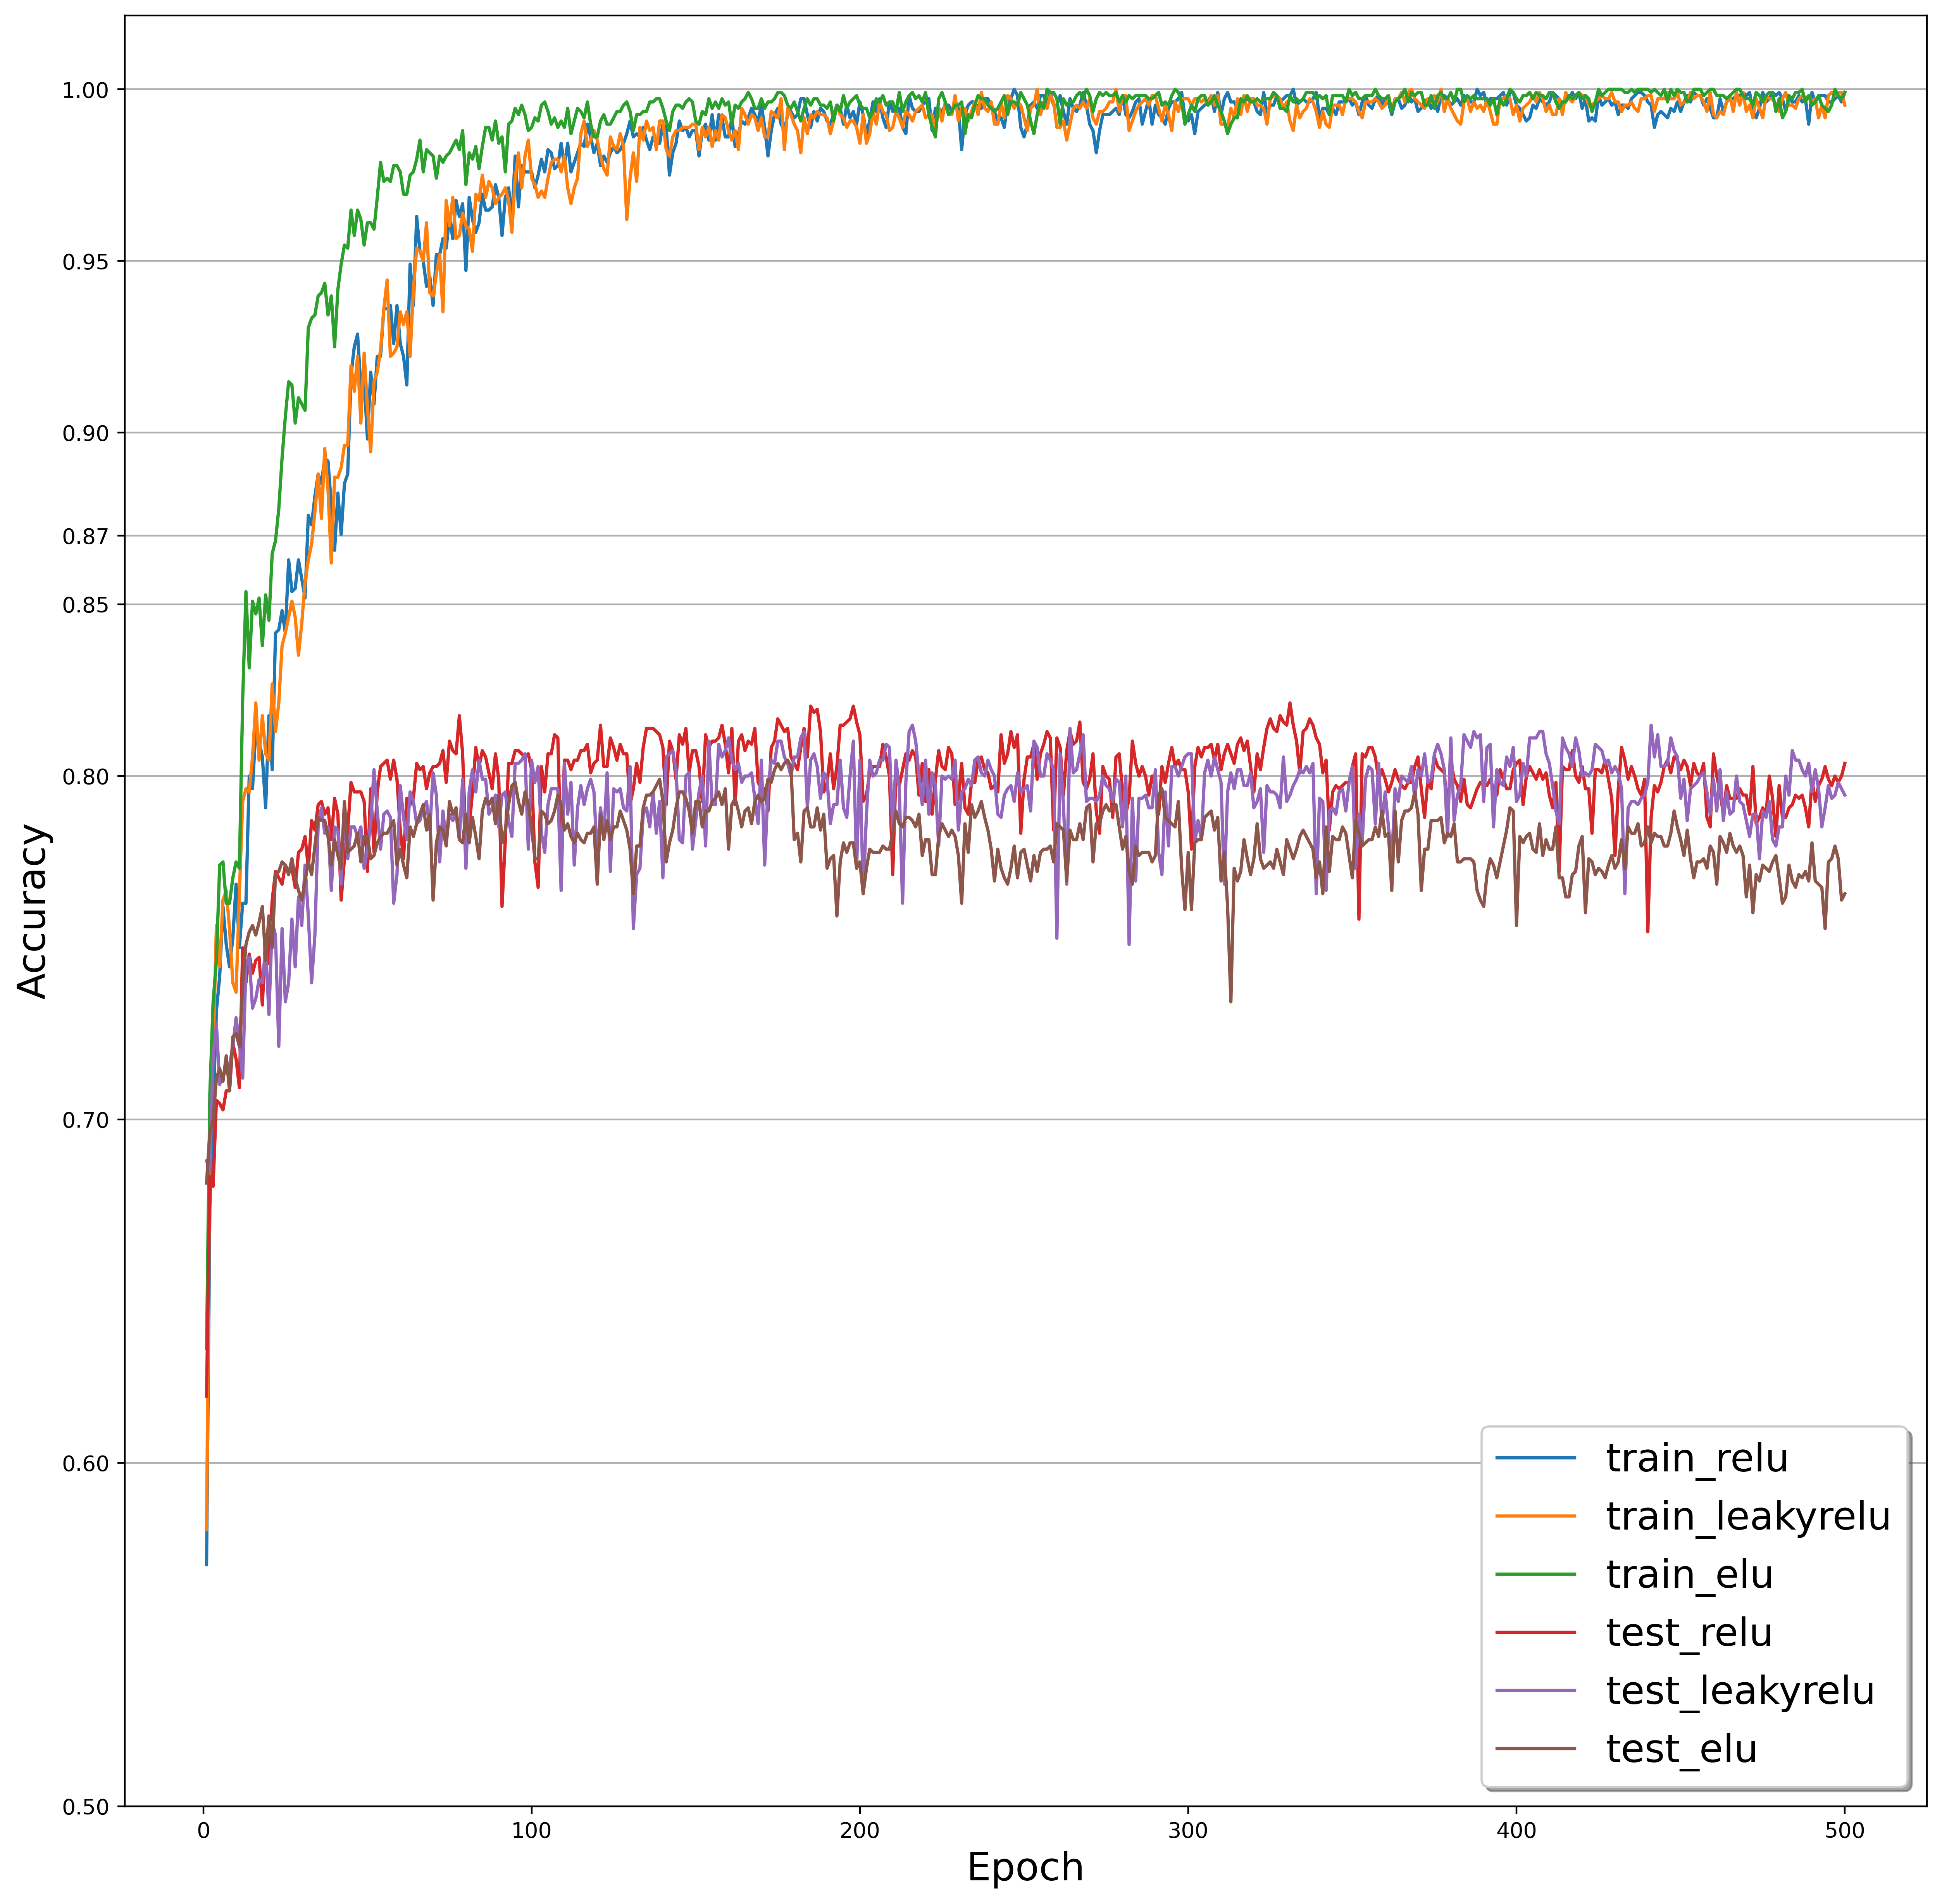
\includegraphics[width=0.45\textwidth]{results/deepconvnet_adam_64_0.0005_0.25_acc.png}
		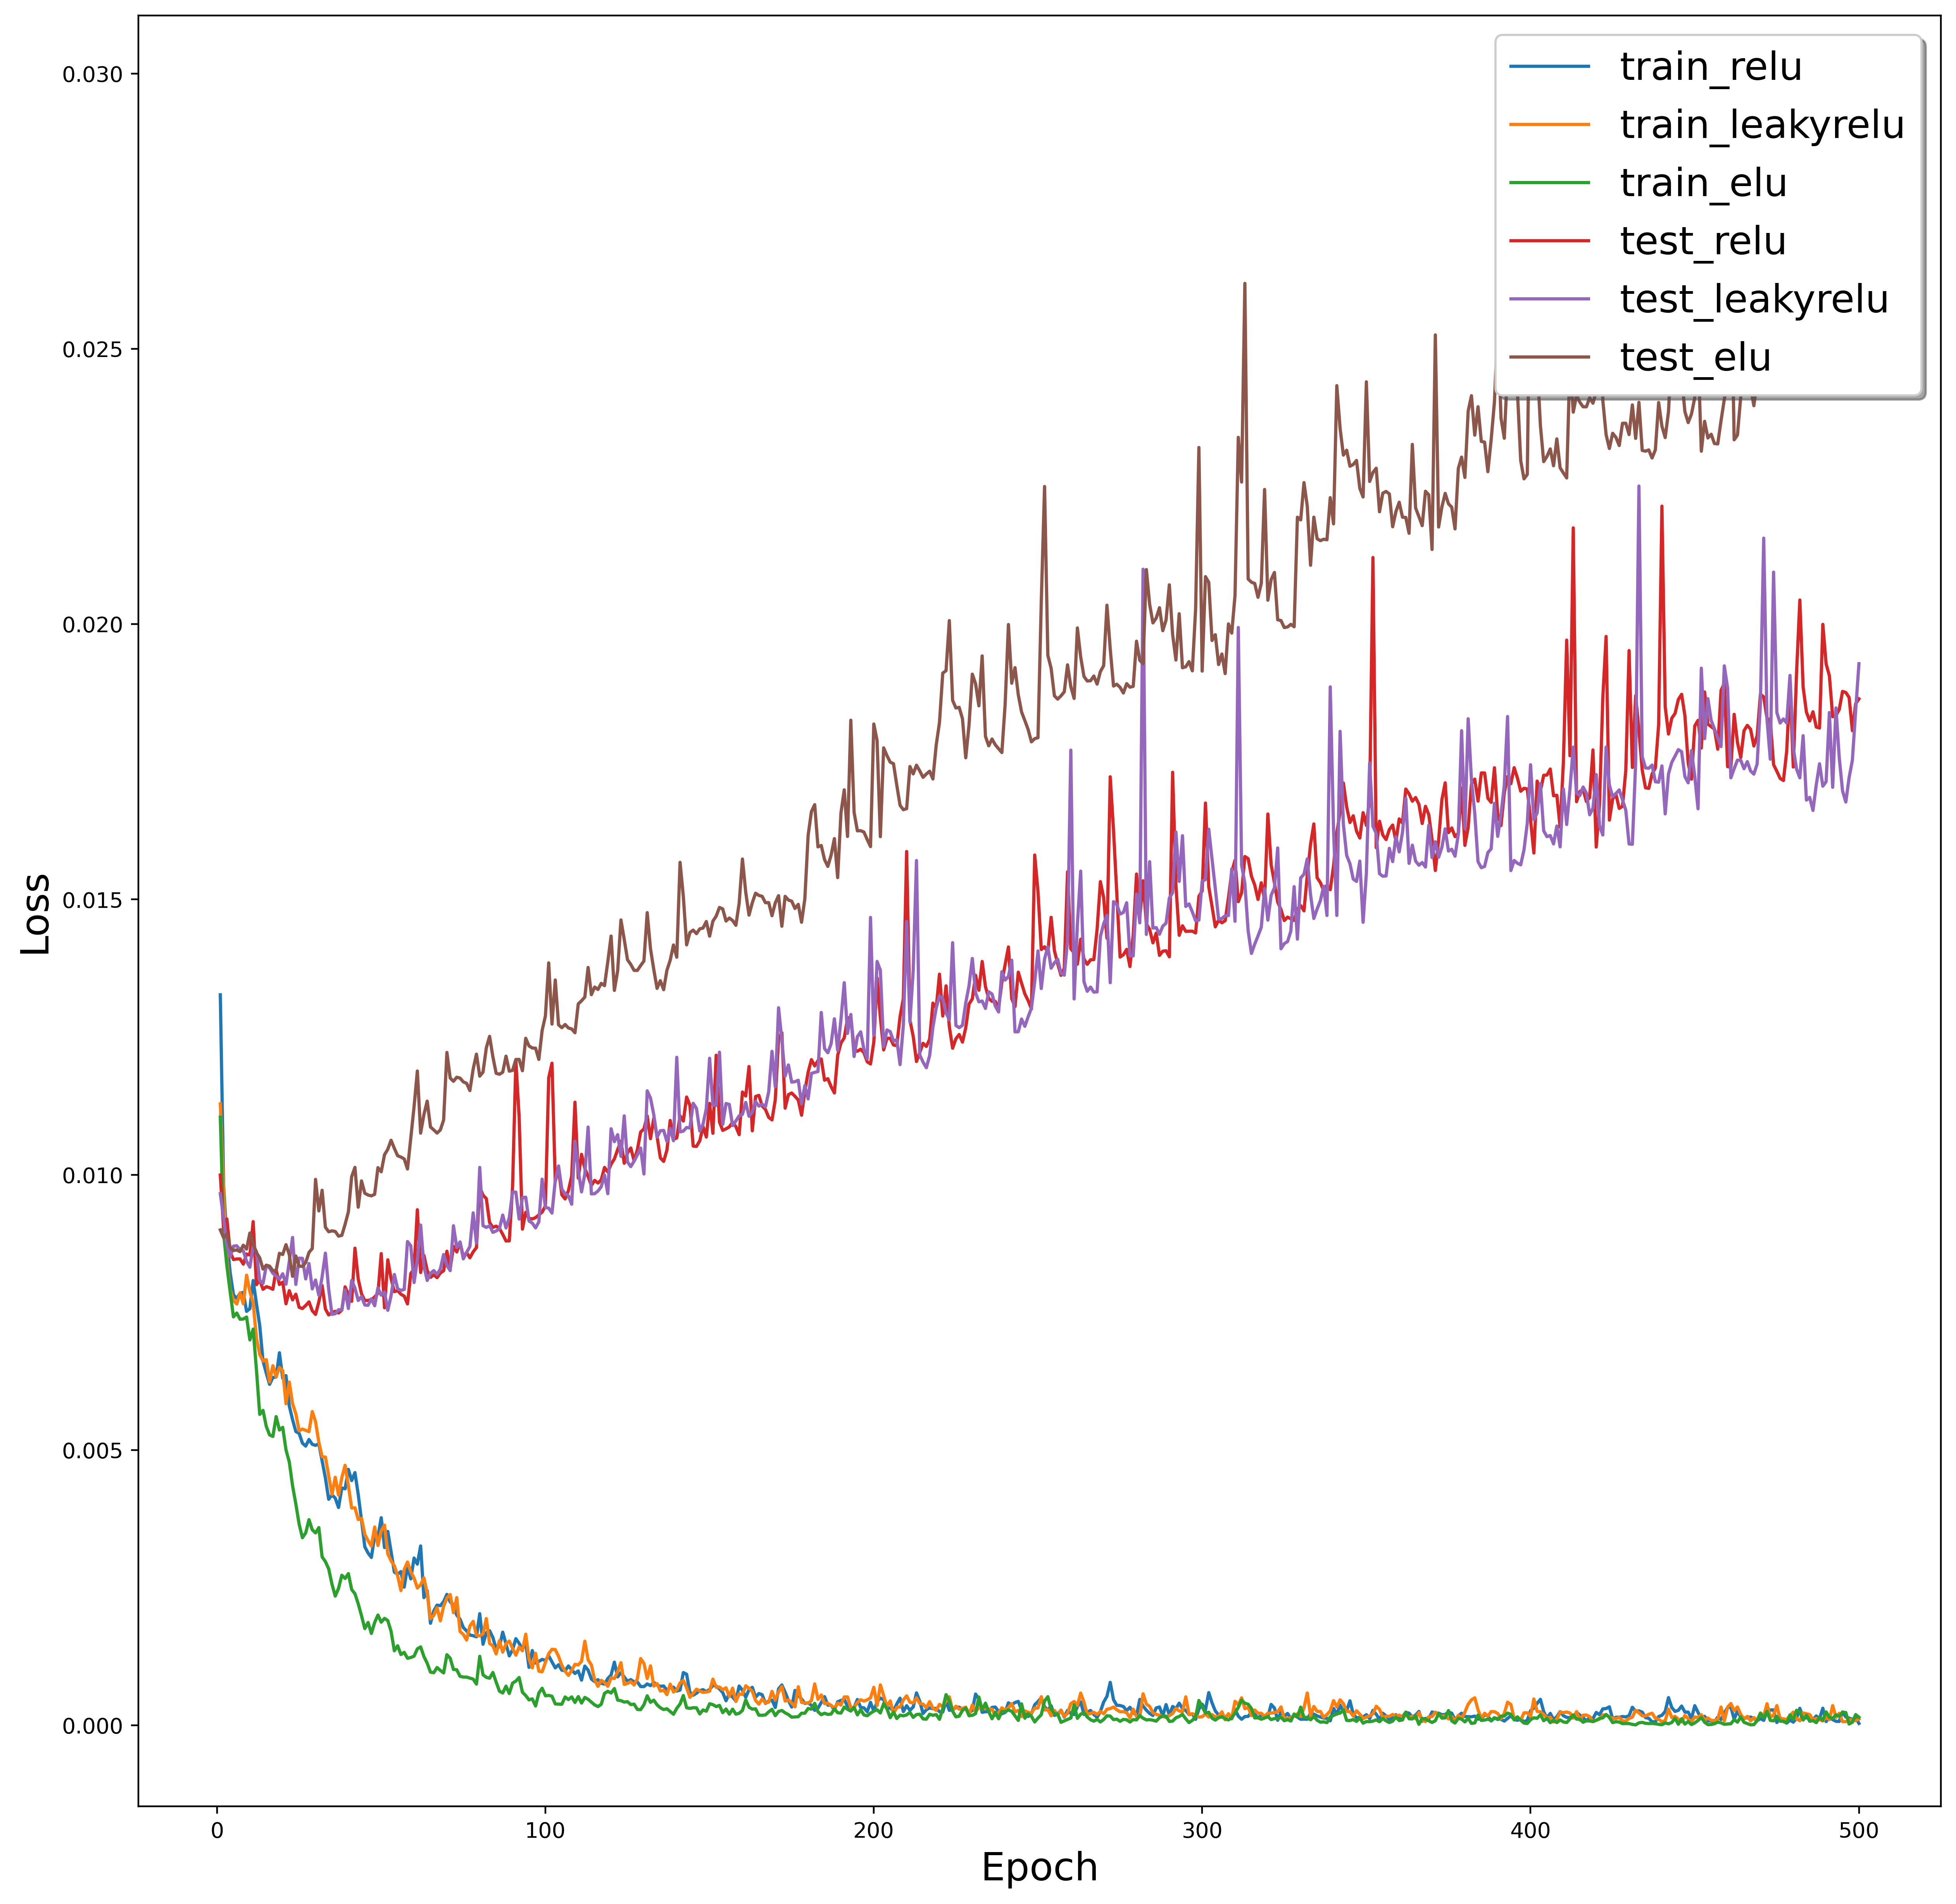
\includegraphics[width=0.45\textwidth]{results/deepconvnet_adam_64_0.0005_0.25_loss.png}
		\caption{DeepConvNet with Adam, 64 batch size, \\ $5 \times 10^{-4}$ learning rate, and 25\% dropout.}
	\end{figure}
	\begin{figure}[H]
		\centering
		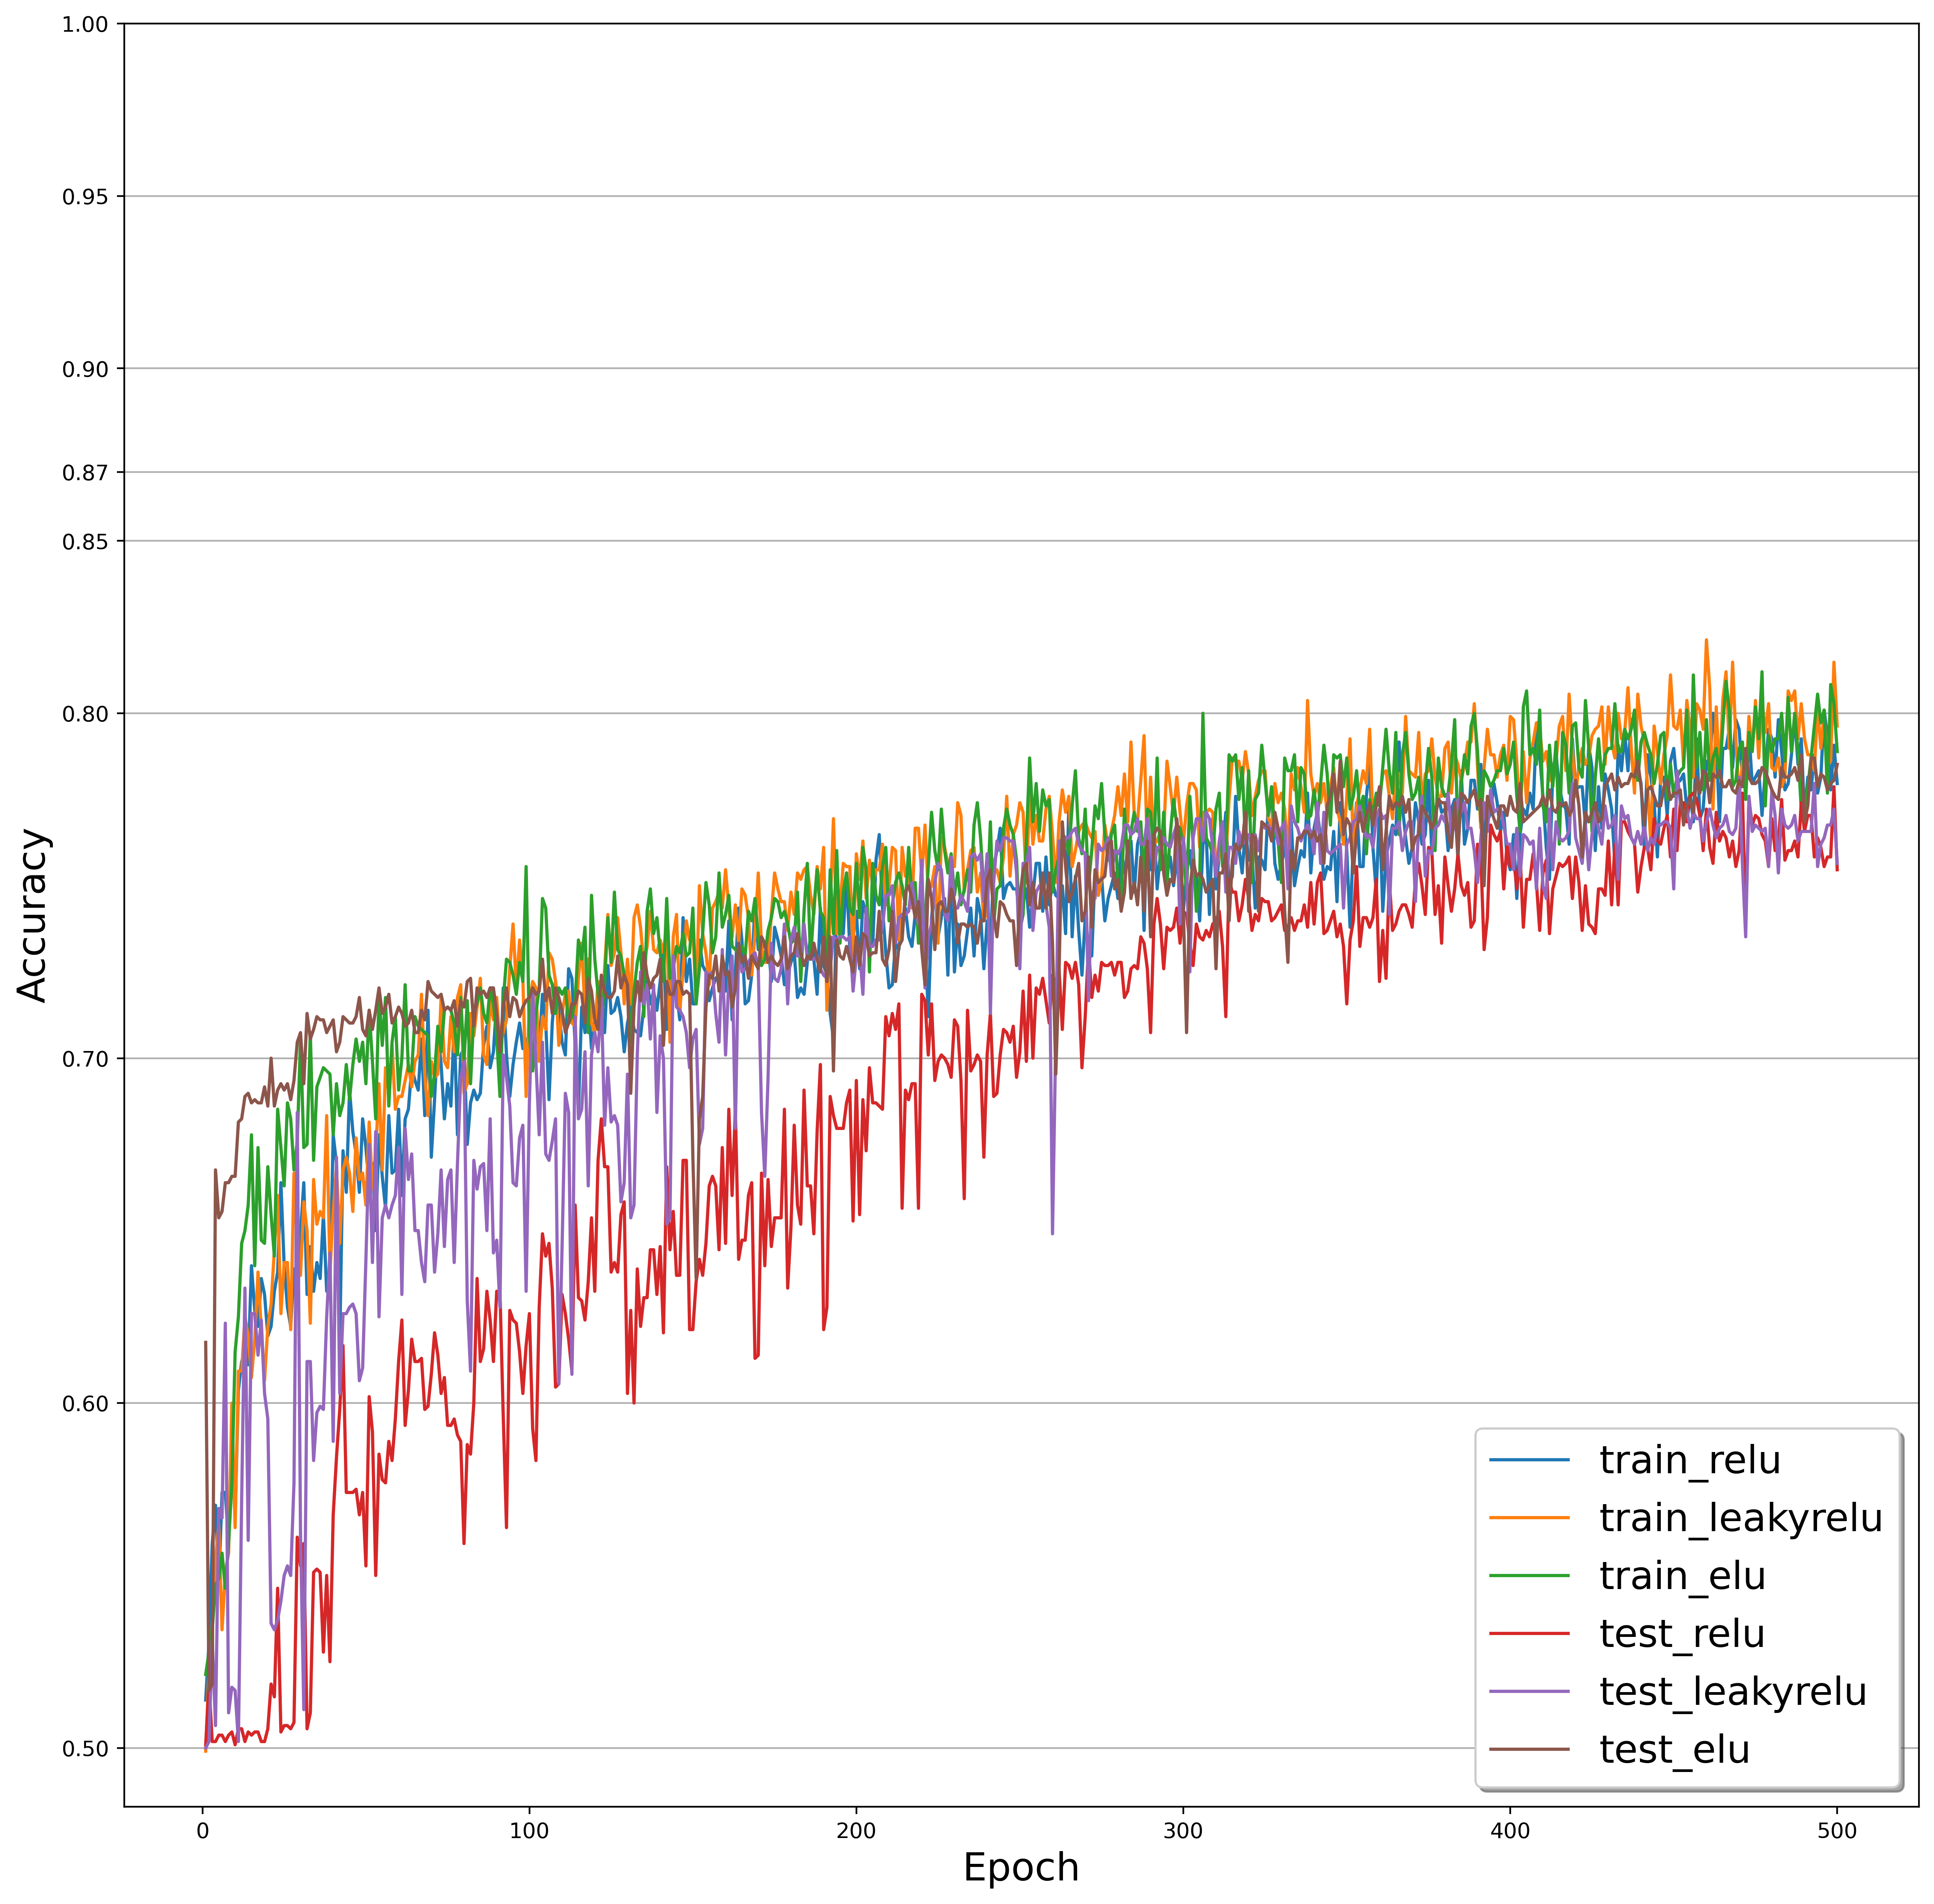
\includegraphics[width=0.45\textwidth]{results/deepconvnet_adam_64_0.0005_0.75_acc.png}
		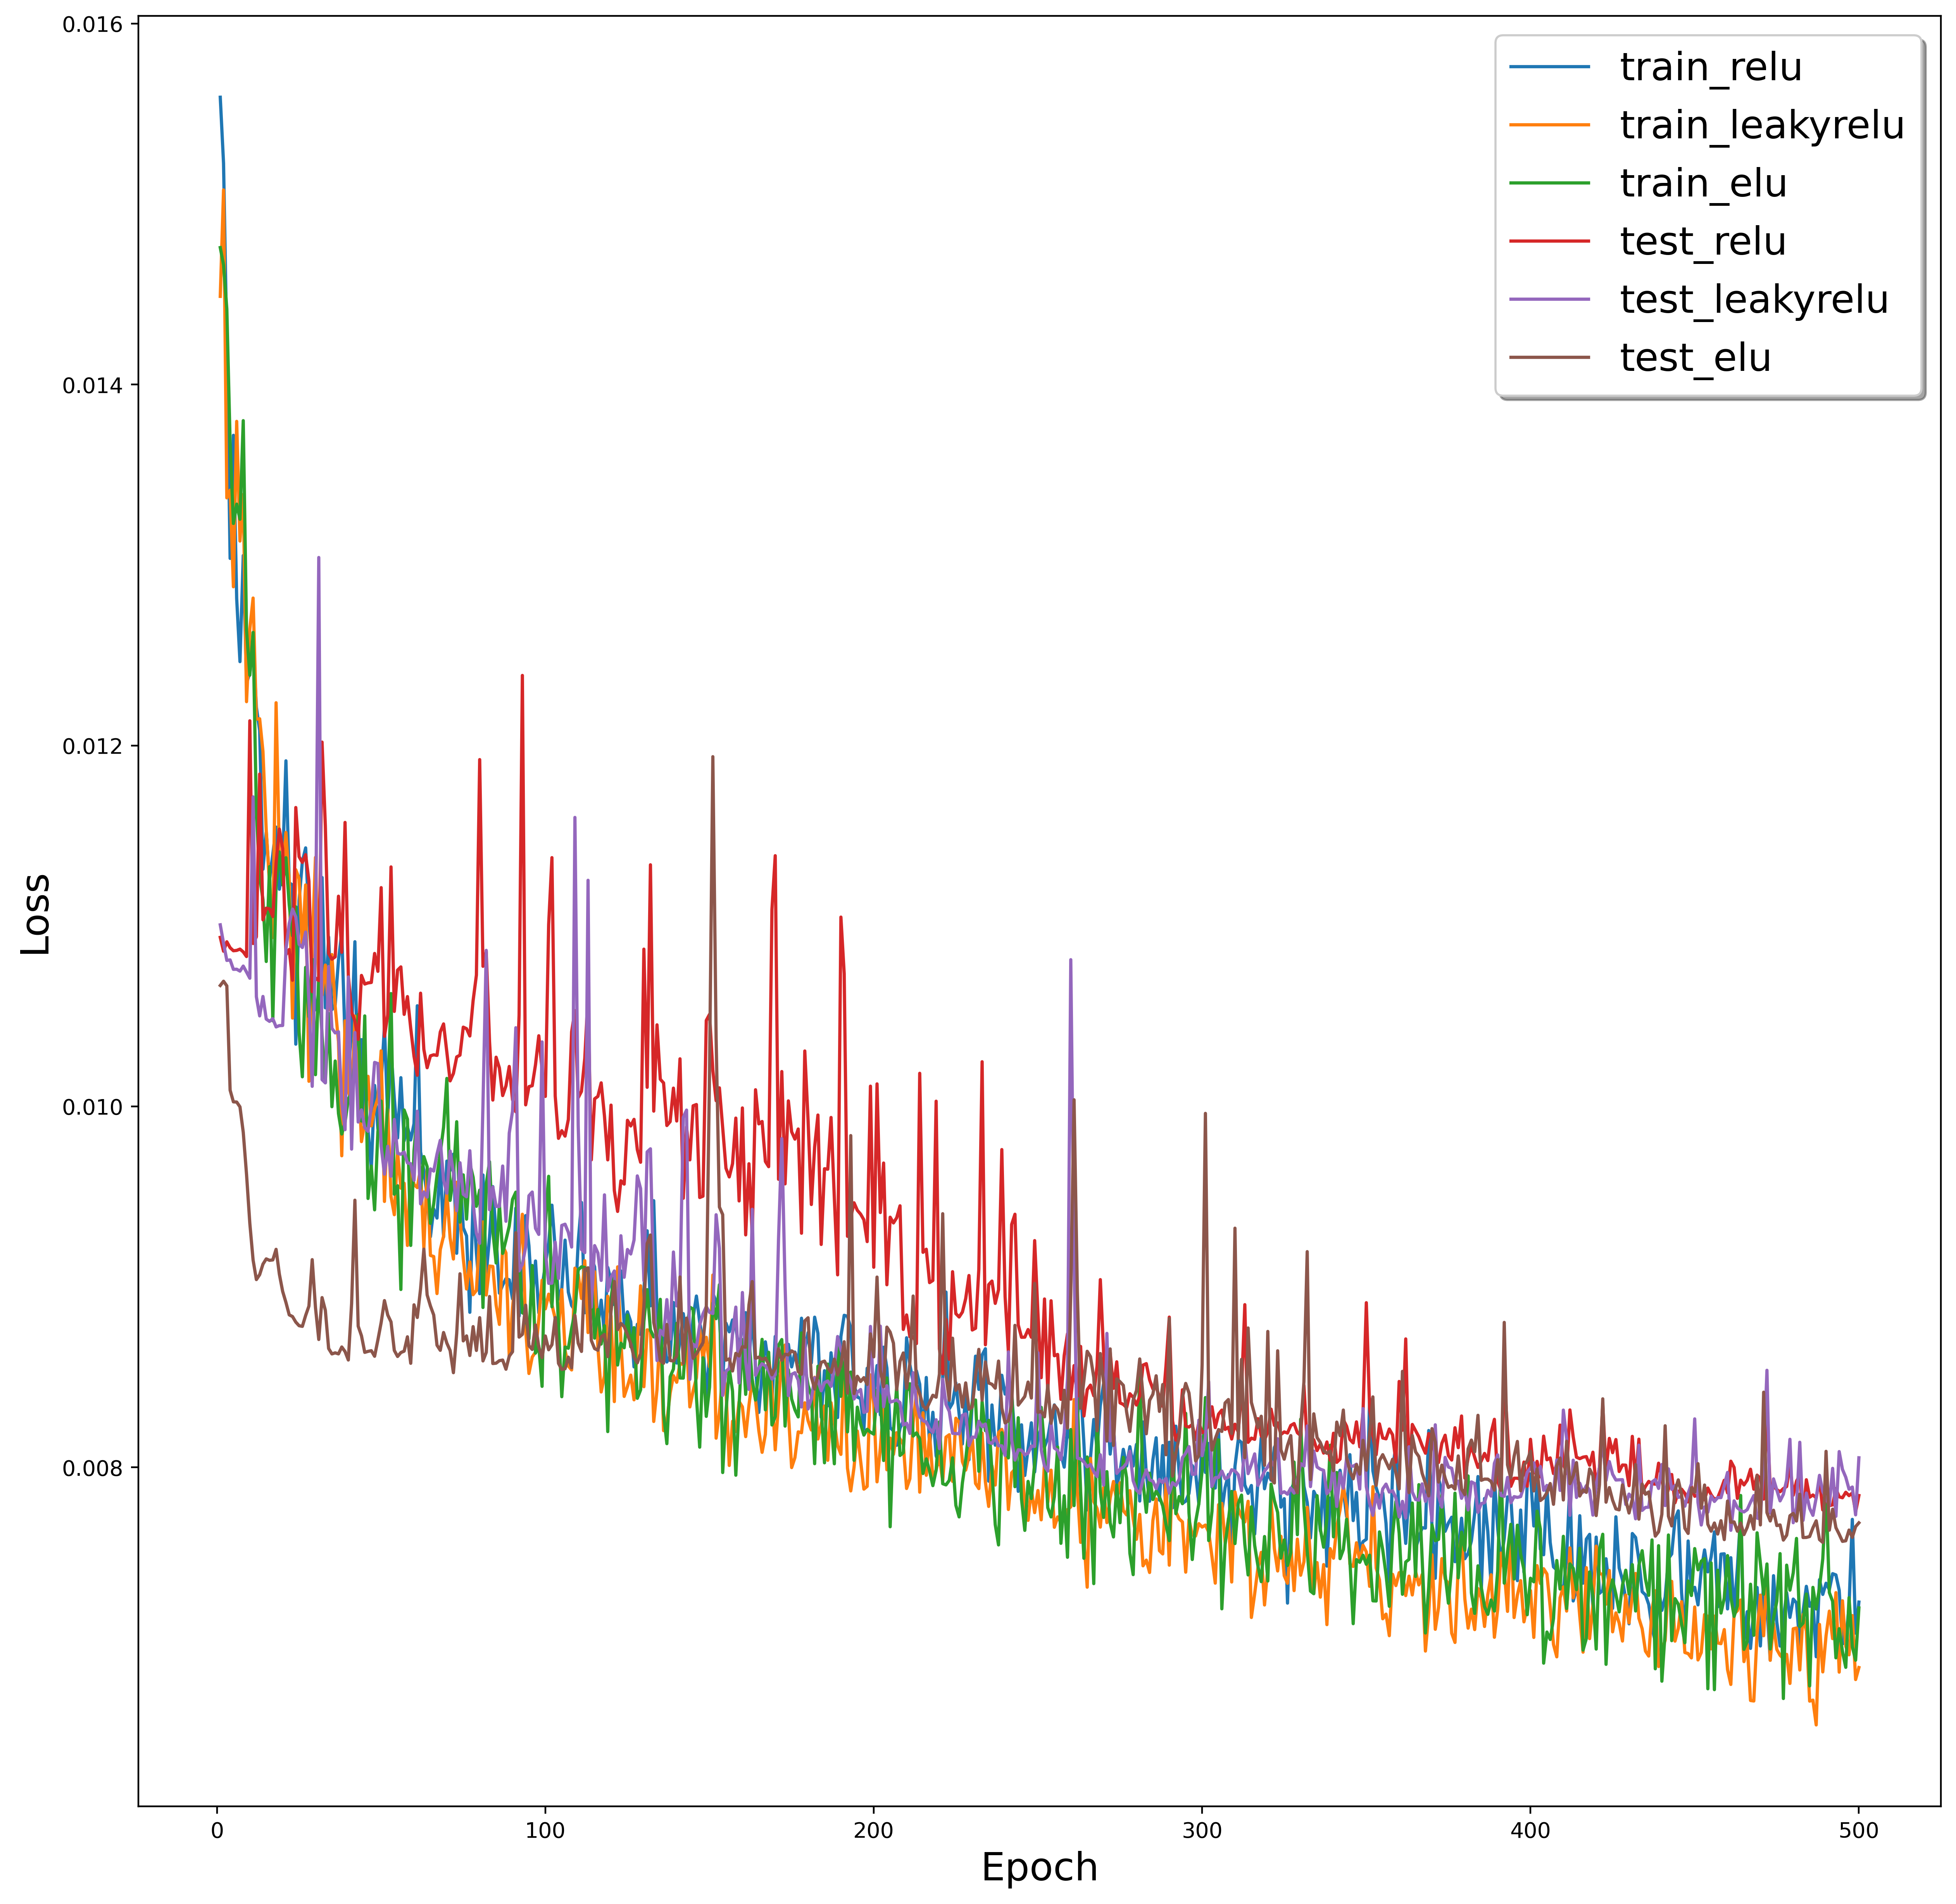
\includegraphics[width=0.45\textwidth]{results/deepconvnet_adam_64_0.0005_0.75_loss.png}
		\caption{DeepConvNet with Adam, 64 batch size, \\ $5 \times 10^{-4}$ learning rate, and 75\% dropout.}
	\end{figure}

	\end{appendices}
\end{document}
